%%%%%%%%%%%%%%%%%%%%%%%%%%%%%%%%%%%%%%%%%
% Daily Laboratory Book
% LaTeX Template
%
% This template has been downloaded from:
% http://www.latextemplates.com
%
% Original author:
% Frank Kuster (http://www.ctan.org/tex-archive/macros/latex/contrib/labbook/)
%
% Important note:
% This template requires the labbook.cls file to be in the same directory as the
% .tex file. The labbook.cls file provides the necessary structure to create the
% lab book.
%
% The \lipsum[#] commands throughout this template generate dummy text
% to fill the template out. These commands should all be removed when 
% writing lab book content.
%
% HOW TO USE THIS TEMPLATE 
% Each day in the lab consists of three main things:
%
% 1. LABDAY: The first thing to put is the \labday{} command with a date in 
% curly brackets, this will make a new page and put the date in big letters 
% at the top.
%
% 2. EXPERIMENT: Next you need to specify what experiment(s) you are 
% working on with an \experiment{} command with the experiment shorthand 
% in the curly brackets. The experiment shorthand is defined in the 
% 'DEFINITION OF EXPERIMENTS' section below, this means you can 
% say \experiment{pcr} and the actual text written to the PDF will be what 
% you set the 'pcr' experiment to be. If the experiment is a one off, you can 
% just write it in the bracket without creating a shorthand. Note: if you don't 
% want to have an experiment, just leave this out and it won't be printed.
%
% 3. CONTENT: Following the experiment is the content, i.e. what progress 
% you made on the experiment that day.
%
%%%%%%%%%%%%%%%%%%%%%%%%%%%%%%%%%%%%%%%%%

%---------------------------------------------------------------------
%	PACKAGES AND OTHER DOCUMENT CONFIGURATIONS
%----------------------------------------------------------------------

\documentclass[idxtotoc,hyperref,openany,oneside]{labbook} % 'openany' here removes the gap page between days, erase it to restore this gap; 'oneside' can also be added to remove the shift that odd pages have to the right for easier reading

\usepackage[ 
  backref=page,
  pdfpagelabels=true,
  plainpages=false,
  colorlinks=true,
  bookmarks=true,
  pdfview=FitB]{hyperref} % Required for the hyperlinks within the PDF
  
\usepackage{booktabs} % Required for the top and bottom rules in the table
\usepackage{float} % Required for specifying the exact location of a figure or table
\usepackage{graphicx} % Required for including images
\usepackage{lipsum} % Used for inserting dummy 'Lorem ipsum' text into the template
\usepackage{mathrsfs}
\usepackage{amsmath}
\usepackage{soul}
\usepackage{wasysym}
\usepackage{bm}
%\usepackage[normalem]{ulem}
%\newcommand{\stkout}[1]{\ifmmode\text{\sout{\ensuremath{#1}}}\else\sout{#1}\fi}
\usepackage{caption}
\captionsetup{labelformat=empty}


\newcommand{\HRule}{\rule{\linewidth}{0.5mm}} % Command to make the lines in the title page
\setlength\parindent{0pt} % Removes all indentation from paragraphs

\usepackage{enumitem,amssymb}
\newlist{todolist}{itemize}{2}
\setlist[todolist]{label=$\square$}
\usepackage{pifont}
\newcommand{\cmark}{\ding{51}}%
\newcommand{\xmark}{\ding{55}}%
\newcommand{\done}{\rlap{$\square$}{\raisebox{2pt}{\large\hspace{1pt}\cmark}}%
  \hspace{-2.5pt}}
\newcommand{\wontfix}{\rlap{$\square$}{\large\hspace{1pt}\xmark}}
\newcommand{\tss}{\textsuperscript}
\newcommand{\tsbs}{\textsubscript}

%---------------------------------------------------------------------
%	DEFINITION OF EXPERIMENTS
%---------------------------------------------------------------------

\newexperiment{Notes}{Experiment Notes}
\newexperiment{Stock}{Stock creation}
\newexperiment{Process1Prep}{Preparation for Process 1}
\newexperiment{Process1_Fail}{Process 1 Mistake experiment}
\newexperiment{Process1_Fail_Counting}{Counting for Process 1
  Mistake experiment (Gamma)}
\newexperiment{Process1_Fail_Counting2}{Counting for Process 1
  Mistake experiment (Alpha)}
\newexperiment{Process1_Fail_Counting_Analysis}{Analysis
  for Process 1 Mistake (Gamma)}
\newexperiment{Cycle_X3_Prep}{Preparation for 3 Cycles}
\newexperiment{table1}{Isotopes we are looking for}
\newexperiment{Cycle_X3}{Cycle experiment, replicate of 3}
\newexperiment{programs}{Calculation Work}
\newexperiment{Contamination}{Contamination spill 10/25/16}
\newexperiment{Contamination2}{Minor Contamination of HPGe,
  found Monday 10/31/2016}
\newexperiment{ResearchMeeting}{Details from research meeting}
\newexperiment{Cycle_X3_round_2}{Cycle experiment, round 2,
  replicate of 3}
\newexperiment{Cycle_X3_round_2_alpha}{Cycle experiment, round 2,
  replicate of 3, ALPHA preparation for
  extraction 1 (also Mass Spec preparation)}
\newexperiment{Process_X3}{Process Experiment (continuation from
  cycle experiment)}
\newexperiment{School}{Things to do for school}
\newexperiment{56_run}{Experiment to double check \tss{137}Cs
  using combined aqueous series 5 and 6, 56}
\newexperiment{Cycle_X3_round_2_alpha_ex2}{Cycle experiment, round 2,
  replicate of 3, ALPHA EXTRACTION II (also Mass Spec preparation)}
\newexperiment{ToCheckout}{Things to Check}
\newexperiment{Alpha_and_MassSpec}{Prepare Alpha chips for counting,
  the mass spec solutions for shipping, count the final combined aqueous
  phases}
\newexperiment{CHEMLAB}{Work that is paying me this semester}
\newexperiment{Buy}{Things we need to buy}
\newexperiment{Grad}{Documents and things for graduation}
%\newexperiment{shorthand}{Description of the experiment}

%----------------------------------------------------------------------
\begin{document}

%----------------------------------------------------------------------
%	TITLE PAGE
%-----------------------------------------------------------------------

\frontmatter % Use Roman numerals for page numbers
\title{
\begin{center}
\HRule \\[0.4cm]
{\Huge \bfseries Laboratory Journal }\\[0.4cm] % Degree
\HRule \\[1.5cm]
\end{center}
}
\author{\Huge Paul Mendoza \\ \\ \LARGE paul.m.mendoza@gmail.com \\[2cm]}
\date{This notebook begins 6 October 2016} 
\maketitle

\tableofcontents

\mainmatter 

%------------------------------------------------------------------------
%	LAB BOOK CONTENTS
%------------------------------------------------------------------------




%------------------------------------------------------------------------
%	LAB BOOK day
%-----------------------------------------------------------------------

\labday{Thursday, 6 October 2016\\ 8:30am - 11:00 am\\ 1:30pm - 3:30pm}

\experiment{table1}
\begin{itemize}
\item{Decay Monitors}
  \begin{itemize}
  \item{\tss{137}Cs/\tss{133}Cs}
  \end{itemize}
\item{Burnup Monitor}
  \begin{itemize}
  \item{(\tss{154}Eu/\tss{153}Eu) [\tss{155}Eu]}
  \end{itemize}
\item{Reactor type monitors}
  \begin{itemize}
  \item{(\tss{134}Cs/\tss{137}Cs)}
  \item{(\tss{150}Sm/\tss{149}Sm)}
  \item{(\tss{242}Pu/\tss{239}Pu)}
  \item{(\tss{135}Cs/\tss{137}Cs)}
  \item{(\tss{136}Ba/\tss{138}Ba)}
  \end{itemize}
\item{Isotope Solve list}
\end{itemize}

\begin{table}[H]
\begin{center}
\begin{tabular}{l l l}
\toprule
\tss{133}Cs & \tss{136}Ba & \tss{153}Eu\\ 
\tss{134}Cs & \tss{138}Ba & \tss{154}Eu\\
\tss{135}Cs & \tss{149}Sm & \tss{239}Pu\\
\tss{137}Cs & \tss{150}Sm & \tss{242}Pu\\
\bottomrule
\end{tabular}
\caption{Isotope solve list.}
\end{center}
\end{table}  

\experiment{Notes}

\begin{itemize}
\item{Project Number: 504370-0001}
\item{EHS Contact:}
  \begin{itemize}
  \item{d-imenchaca@tamu.edu}
  \item{979-676-0590 For Dan}
  \item{979-845-2132:General}
  \end{itemize}
\item{Files on computer saved in C:/Paul\_Mendoza}
\item{\tss{152}Eu Liquid calibration source}
  \begin{itemize}
  \item{Source 1577-22}
  \item{497.0 nCi}
  \item{Assy Date: 15 Feb 12}
  \item{1.00568g}
  \end{itemize}
\item{Stock HNO\tsbs{3}: Assuming Temp=24.8+/-3 $\rightarrow\boxed{Stock\ HNO_3}$}
  \begin{itemize}
  \item{Molarity : 15.35+/-0.13}
  \item{pH: -1.186+/-0.004}
  \item{Molality: 35.3+/-0.8}
  \item{Wt Concentration: 69.0+/-0.5}
  \item{Molar Mass: 63.0130+/-0.0012}
  \item{Density: 1.402+/-0.006}
  \end{itemize}
\item{Stock Iron Sulfamate $Fe(NH_2SO_3)_2$ $\rightarrow\boxed{Stock\ Fe(II)}$}
  \begin{itemize}
  \item{Molarity : 2.302+/-0.009}
  \item{Molality : 2.717+/-0.006}
  \item{Wt Concentration : 40.26+/-0.05}
  \item{Molar Mass : 248.022+/-0.017}
  \item{Density: 1.418+/-0.005}
  \end{itemize}
\end{itemize}

\experiment{Stock} % 

\begin{itemize}
\item{Get stock solution from Troy room 18A, store near rad waste}
\item{Grab 1000$\mu$l pipett from glovebox}
\item{Decontaminate with radic - dump waste into glass aq rad outside glove box}
\item{Practice pipetting 500$\mu$l to glass vial - setting 503 $\mu$l
  gives 500 $\mu$l}
\item{Class/lunch Break}
\item{Get alpha detector from Dr. Marianno}
\item{Set up laboratory notebook}
\item{Calculation}
  To do calculation to determine the volumes needed for a final
  concentration of a particular volume, knowing the initial
  concentrations
  \begin{align*}
    V_2&=\frac{b_2-\frac{M_1b_1}{A}}{M_2-\frac{M_1}{A}}\\
    V_1&=\frac{b-BV_2}{A}
  \end{align*}
  Where:
  \begin{align*}
    A&=(1-wt\%_1)\rho_1\\
    B&=(1-wt\%_2)\rho_2\\
    b_1&=(1-wt\%_3)V_3\rho_3\\
    b_2&=M_3V_3
  \end{align*}
  With known Molarity and volume of a solution
  how much, and of what concentration
  do we need to combine with a second solution
  to get a final solution of known concentration
  and volume?
  \begin{align*}
    B&=(1-wt\%_3)V_3\rho_3-(1-wt\%_1)V_1\rho_!\\
    A&=M_3V_3-M_1V_1\\
    C&=\frac{B}{A}=\frac{(1-wt\%_2)\rho_2}{M_2}
  \end{align*}
  Need iterative solution, choose:
  \begin{align*}
    M_2&=\frac{M_3V_3-M_1V_1}{V_3-V_1}\\
    V_2&=V_3-V_1
  \end{align*}
  Use to determine molality $\rightarrow$ $wt\%_2$ $\rightarrow$
  $\rho_2$. Then compare to $C$, iterate around the solution to
  find answer so that $C=\frac{(1-wt\%_2)\rho_2)}{M_2}$.
\end{itemize}

%------------------------------------------------------------------------
%	LAB BOOK day
%-----------------------------------------------------------------------

\labday{Friday, 7 October 2016\\ 9:00am - 12:00 am\\ 1:00pm - 4:00pm}

\experiment{Stock} % 

\begin{todolist}
\item[\done]{Program calculation for creation of stock - some
results shown below}
\item[\done]{Prepare shielding for transfer for closet solution}
  \begin{itemize}
  \item{Clean off and move leaded shielding in rad area to
    countertop next to fumehood}
  \item{Add diaper paper on countertop, and on shielding incase
    of contamination}
  \item{Practice transfer}
  \end{itemize}
\item[\done]{-}
\end{todolist}
\begin{center}
    0.149+/-0.011 ml of 15.43+/-0.06 M HNO\tsbs{3} $\boxed{Stock\ HNO_3}$\\
    +\\
    1.91+/-0.08  ml of 0.0+/-0 M solution $\boxed{DI\ Water}$\\
    = \\
    2.048+/-0.026 ml of 1.12+/-0.08 M HNO\tsbs{3}
  solution $\boxed{\rightarrow Stock}$ (glass container)
\end{center}
\begin{todolist}
\item[\done]{-}
\end{todolist}
\begin{center}
Combine 0.500+/-0.005 ml of 15.43+/-0.06 M HNO\tsbs{3}
solution $\boxed{closet}$\\
+\\
2.048+/-0.026 ml of 1.12+/-0.08 M HNO\tsbs{3} solution
$\boxed{Stock}$
\\
=\\
2.500+/-0.025 ml of 4.00+/-0.05 M HNO\tsbs{3} solution.
$\boxed{\rightarrow Stock}$
\end{center}

\begin{todolist}
\item[\done]{Lock $\boxed{Stock}$ in glovebox}
\item[\done]{Put Source back in rad closet}
\item[\done]{Clean up contamination added to pipette tip from transfer (for some reason, the contamination was added to the inside of the pipette itself, the tips used don't have the block, but still, none of the solution should have traveled up the shaft}
\item[\done]{Dispose of diaper paper laid down for transfer (where the glass bottle was set down which contained closet solution, there was contamination (the outside of the bottle of the closet solution is contaminated)}
\item[\done]{Move shielding back to where it was}
\end{todolist}

\experiment{Process1Prep}
\begin{todolist}
\item[\done]{Count calibration standard Eu-152 in HPGe 3 hours 22 minutes at furtherest position from detector (26 cm)}
  \begin{itemize}
  \item{Source 1577-22}
  \item{497.0 nCi}
  \item{Assy Date: 15 Feb 12}
  \item{1.00568g}
  \end{itemize}
\item[\done]{Create Eu-152 Excel Counting sheet template for standards}
\item[\done]{Set up ROI (region of interest) file for Eu-152}
\item[\done]{Start background count and done for the day}
  \begin{itemize}
  \item{Count lasted for 12 hours}
  \end{itemize}
\end{todolist}

%------------------------------------------------------------------------
%	LAB BOOK day
%-----------------------------------------------------------------------

\labday{Saturday, 8 October 2016\\ 10:00am - 2:00 pm}

\experiment{Process1Prep}

\begin{todolist}
\item[\done]{Finish background count, lasted 12 hours}
\item[\done]{Remove 0.3 ml from $\boxed{Stock}$ transfer to $\boxed{1}$
  for counting}
  \begin{itemize}
  \item{$\boxed{1}$ is a smaller tube, which will fit into a larger
    centrifuge tube for, well, centrifuging}
  \item{$\boxed{1}$ tube cannot fit into centrifuge tube with white
    push cap (pushes on outside of tube),
    white push cap is necessary when votex mixing, so a blue push cap
    (pushes on inside of tube), was put on for counting, these smaller
    tubes will have to have two caps following them around, I can't
    wait till the second cycle when the bigger tubes will be used}
  \item{Note for why smaller tubes are being used: when pipetting the
    smaller volume of 0.3 ml for aq/o phase separation it is much
    easier to have the smaller diameter tubes}
  \item{Stock was removed from glovebox, and after was put into the safe}
  \end{itemize}
\item[\done]{Count $\boxed{1}$ for 1 hour and 24 minutes}
\item[\done]{Fix density calculation in code, was slightly wrong before,
  this means $\boxed{Stock}$ and $\boxed{1}$ are slightly different
  from what they should be, but within error}
\item[\done]{Calculation for creation of Fe(II) solution (next page)}
\end{todolist}
\clearpage
\begin{center}
  $V_1$ ml of $M_{1,Fe}$ Fe(II) in $M_{1,HNO_3}$ HNO\tsbs{3}\\
  $+$\\
  $V_2$ ml of $M_{2,Fe}$ Fe(II) in $M_{2,HNO_3}$ HNO\tsbs{3}\\
  =\\
$V_3$ ml of $M_{3,Fe}$ Fe(II) in $M_{3,HNO_3}$ HNO\tsbs{3}.
\end{center}

The knowns are: \\
$M_{1,Fe}=2.302$, $\rho_1=1.418$, $M_{1,HNO_3}=0$ (Fe Stock soltuion)\\
$M_{2,Fe}=0$,$\rho_2=\rho_{HNO_3}(M_{2,HNO_3})$ \\
$V_3=4$ ml, $M_{3,Fe}=0.024$, $M_{3,HNO_3}=4$, $\rho_3=\rho_{HNO_3}(4M)$\\~\\

Mols of Fe(II) constant: $V_1=\frac{M_{3,Fe}V_3}{M_{1,Fe}}=0.042$\\
Mols of HNO\tsbs{3} constant: $V_2=\frac{V_3M_{3,HNO_3}}{M_{2,HNO_3}}$\\
Mass Constant: $V_2=\frac{V_3\rho_3-V_1\rho_1}{\rho_2}$\\~\\

Combine last two equations:$M_{2,HNO_3}-
\frac{V_3M_{3,HNO_3}\rho_2}{V_3\rho_3-V_1\rho_1}=0$\\~\\
Solve iteratively (where $M_{2,HNO_3}$ determines $\rho_2$)
with first guess of:
$M_{2,HNO_3}=\frac{M_{3,HNO_3}V_3}{V_2}$



%------------------------------------------------------------------------
%	LAB BOOK day
%-----------------------------------------------------------------------

\labday{Sunday, 9 October 2016\\ 7:30 pm - 11:30 pm}

\experiment{Process1Prep}

\begin{todolist}
\item[\done]{Prepare for multi contact extraction and back extraction exp}
  \begin{itemize}
  \item{Make solution of 30 vol.\% TBP with kerosene}
  \item{Make 40 ml of solution 4.06 M HNO\tsbs{3} solution, }
  \item{Transfer two smaller vials (one for TBP phase), one for
    Fe phase, with two different lids into glovebox (with
  a larger vial to hold them in the centrifuge)}
  \item{Transfer two smaller vials with centrifuge vials for
    centrifuging, keep one with water 0.3 ml, and TBP mix 0.32 ml
    $\boxed{Vial\ 1\ Budd}$, and
    the second with 1.2 ml of TBP mix and 1.25 ml water
    $\boxed{Vial\ 2\ Budd}$}
  \item{Transfer $\boxed{Stock}$ and $\boxed{1}$ to glovebox}
  \item{Transfer another vial to hold the Fe solution}
  \item{Make sure tweezers are in glovebox (they are) - to remove smaller
    vials from centrifuge tubes}
  \item{Transfer slightly contaminated pipette to glovebox}
  \item{All above vials that would contain solution were rinsed
    with whatever they would hold for approximately 3 minutes}
  \end{itemize}
\end{todolist}

\begin{todolist}
\item[\done]{-}
\end{todolist}
\begin{center}
15+/-0.15 ml of TBP $\boxed{Stock\ TBP}$\\
+\\
35+/-0.35 ml of kerosene $\boxed{Stock\ kerosene}$\\
=\\
50+/-0.5 ml of 30 vol.\% TBP.
$\boxed{\rightarrow TBP}$
\end{center}

\begin{todolist}
\item[\done]{-}
\end{todolist}
\begin{center}
10.579+/-0.011 ml of 15.35+/-0.13 M HNO\tsbs{3} $\boxed{Stock\ HNO_3}$\\
+\\
30.355+/-0.030 ml of 0.0+/-0 M HNO\tsbs{3} solution $\boxed{DI\ Water}$\\
=\\
39.94+/-0.14 ml of 4.07+/-0.04 M HNO\tsbs{3} solution
$\boxed{\rightarrow Fe\ Prep}$
\end{center}

To create an Fe solution for a back extraction, $\boxed{Fe\ Prep}$ should be
combined in the following manner (Small portions created because this
solution has a short half life with larger concentrations of $HNO_3$).

\begin{todolist}
\item{-}
\end{todolist}
\begin{center}
0.0417+/-0.0018 ml of 2.302+/-0.009 M Fe(II) in 0.0+/-0 M HNO\tsbs{3} $\boxed{Stock\ Fe(II)}$\\
+\\
3.941+/-0.027 ml of 0.0+/-0 M Fe(II) in 4.06+/-0.05 M HNO\tsbs{3} solution $\boxed{Fe\ Prep}$\\
+\\
4.000+/-0.020 ml of 0.0240+/-0.0010 M Fe(II) in 4.00+/-0.05 M HNO\tsbs{3} solution $\boxed{\rightarrow Bk\ Ex\ Solution}$.
\end{center}

\begin{todolist}
\item[\done]{Add Sodium Nitrite to $\boxed{1}$, it will sit overnight,
but it doesn't have to}
  \begin{itemize}
  \item{Dropped $\boxed{1}$, solution probably contaminated blue lid
    (crap), centrifuged on 1000 rpm for 2 minutes}
  \end{itemize}
\end{todolist}


%------------------------------------------------------------------------
%	LAB BOOK day
%-----------------------------------------------------------------------

\labday{Monday, 10 October 2016\\ 12:30 pm - 4:30 pm}

\experiment{Process1_Fail}
\begin{todolist}
\item[\done]{First contact - Extraction}
  \begin{itemize}
  \item{Add 0.32 ml $\boxed{TBP}$ to $\boxed{1}$}
  \item{Shake on Pulse Mode of 15 minutes on vortex mixer}
  \item{Change of plans (This occured while sample settled for
       a bit while changes were implemented)}
    \begin{itemize}
    \item{Put smaller tubes directly into centrifuge - so we do not
      have to switch caps so often}
    \item{Pulled out $\boxed{Vial\ 1\ Budd}$ and $\boxed{Vial\ 2\ Budd}$
      Pulled out of glovebox the smaller tubes,
      changed their caps, labeled them, put back into
      glovebox (5-10 minutes)}
    \end{itemize}
  \item{Centrifuge 1000 rpm for 10 minutes}
  \item{Attempted to pull out 0.30 ml of TBP phase}
    \begin{itemize}
    \item{Utter Failure}
    \item{Utter Failure again}
    \item{Utter failure...difficult to pull out 0.3 ml and keep
    phases separate}
    \end{itemize}
  \item{Added 1.08 ml $\boxed{TBP}$ to $\boxed{1}$ (for 0.2 ml buffer)}
    \begin{itemize}
    \item{All extractions at once (different from original exp)}
      \begin{align*}
        p=\frac{1}{1+\frac{1}{D}\frac{V_{aq}}{V_o}}
      \end{align*}
    \item{$V_o$ increased by fourfold}
    \item{Pipette slipped to 538 (instead of 540 $\rightarrow$ 0.4\%
      increase in error)}
    \end{itemize}
  \item{Vortex mix for 15 minutes on pulse mode}
  \item{Centrifuge 1000 cpm for 10 minutes}
  \item{Remove 1000 ml top phase (TBP), then remove
    another 200 ml of top phase (TBP) $\boxed{\rightarrow 2}$}
  \end{itemize}
\item[\done]{Creation of $\boxed{Bk\ Ex\ Solution}$}
\end{todolist}
\begin{center}
0.0417+/-0.0018 ml of 2.302+/-0.009 M Fe(II) in 0.0+/-0 M HNO\tsbs{3} $\boxed{Stock\ Fe(II)}$\\
+\\
3.941+/-0.027 ml of 0.0+/-0 M Fe(II) in 4.06+/-0.05 M HNO\tsbs{3} solution $\boxed{Fe\ Prep}$\\
+\\
4.000+/-0.020 ml of 0.0240+/-0.0010 M Fe(II) in 4.00+/-0.05 M HNO\tsbs{3} solution $\boxed{\rightarrow Bk\ Ex\ Solution}$.
\end{center}
\begin{todolist}
\item[\done]{Back Extraction - First Contact}
  \begin{itemize}
  \item{Add 1.4 $\boxed{Bk\ Ex\ Solution}$ to $\boxed{2}$}
  \item{Shake pulse mode for 15 minutes}
  \item{Remove 1.2 ml of bottom phase (Fe(II)) $\boxed{\rightarrow 3}$}
    \begin{itemize}
    \item{Lost two drops}
    \item{While placing vial into centrifuge, cap shot off,
      spraying solution everywhere...great}
    \end{itemize}
  \end{itemize}
\item[\done]{Back Extraction - Second Contact}
  \begin{itemize}
  \item{Add 1.2 $\boxed{Bk\ Ex\ Solution}$ to $\boxed{2}$}
  \item{Shake pulse mode for 15 minutes}
  \item{Remove 1.2 ml of bottom phase (Fe(II)) $\boxed{\rightarrow 3}$}
  \end{itemize}
\item[\done]{Back Extraction - Third Contact}
  \begin{itemize}
  \item{Add 1.2 $\boxed{Bk\ Ex\ Solution}$ to $\boxed{2}$}
  \item{Shake pulse mode for 15 minutes}
  \item{Remove 1.2 ml of bottom phase (Fe(II)) $\boxed{\rightarrow 3}$}
  \end{itemize}
\end{todolist}
\vspace{5mm}
This experiment had sputtering of pipette at certain times.

\experiment{Process1_Fail_Counting}
\begin{todolist}
\item[\done]{Counted waste $\boxed{1}$, containing 0.3
  ml of $\boxed{Stock}$ and 0.2 ml $\boxed{TBP}$, on HPGe,
  for 12 hours (left for the night)}
\end{todolist}

\begin{figure}[H] % Example of including images
\begin{center}
  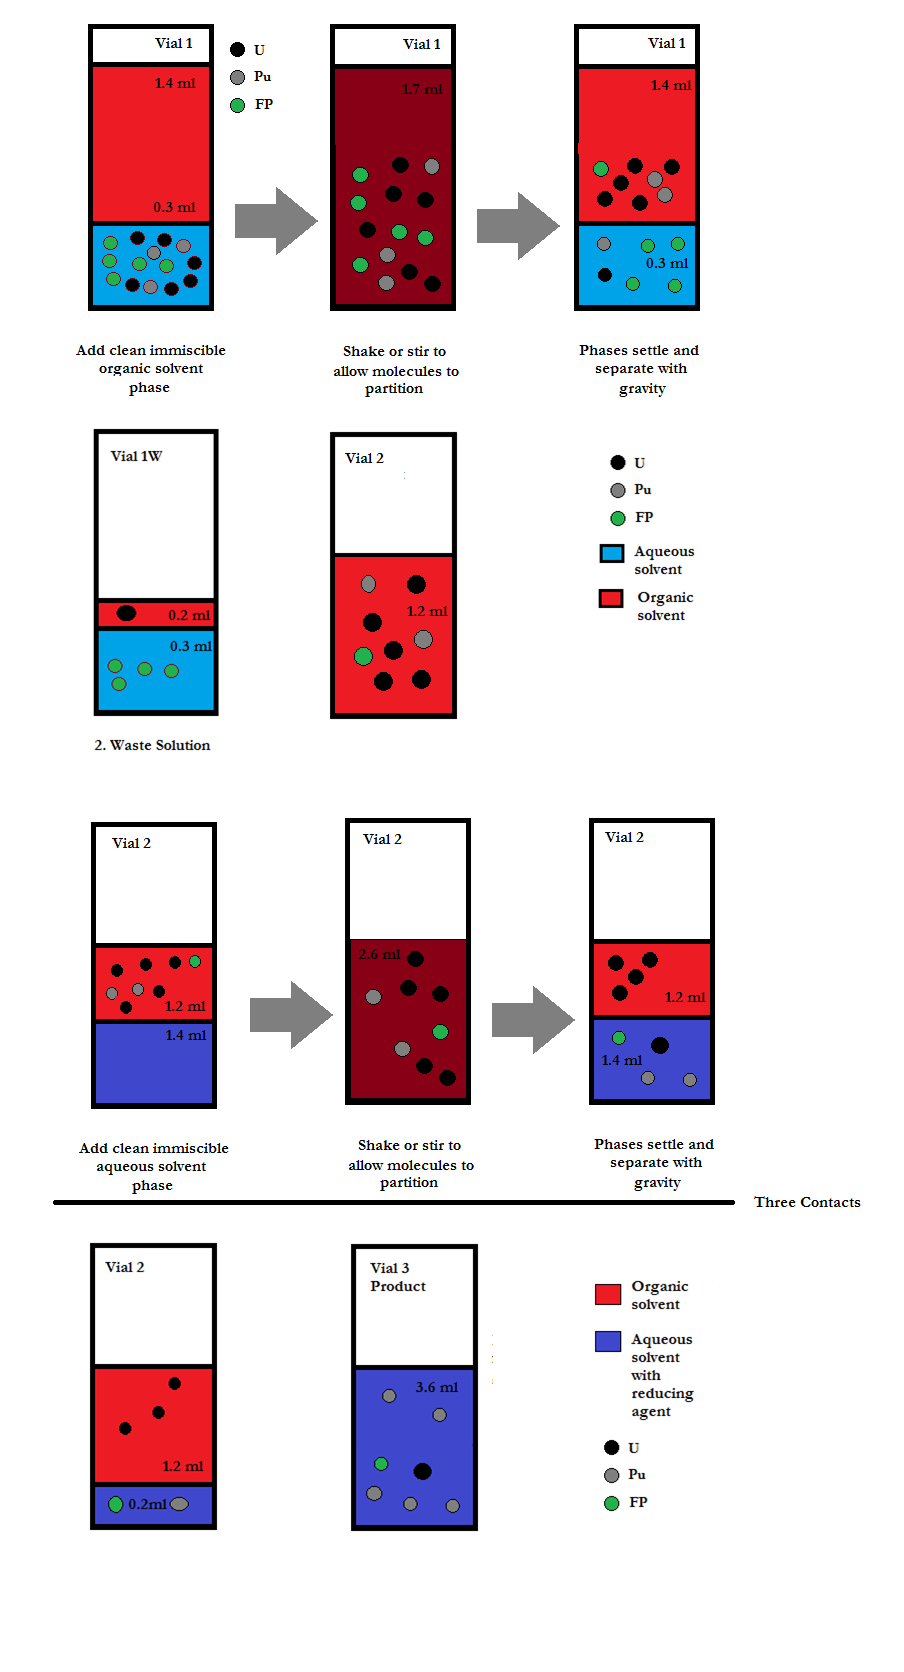
\includegraphics[width=0.85\linewidth]
                  {Figures/Process_1_Mess_Up}
\end{center}
\caption{Process 1 Mess Up Experimental Overview}
\label{fig:example2}
\end{figure}


%------------------------------------------------------------------------
%	LAB BOOK day
%-----------------------------------------------------------------------

\labday{Tuesday, 11 October 2016\\ 10:30 pm - 1:00 am}

\experiment{Process1_Fail_Counting}
There are 6 things to count.
\begin{todolist}
\item[\done]{Initial solution $\boxed{1}$ - 23 cm away, 0.3 ml HNO\tsbs{3}}
\item[\done]{Waste $\boxed{1}$ - 23 cm away, 0.3 ml HNO\tsbs{3} 0.2 ml TBP}
\item[\done]{Create 4 M HNO\tsbs{3} solution store in fume hood}
\end{todolist}
\begin{center}
2.6056+/-0.0026 ml of 15.35+/-0.13 M HNO\tsbs{3} solution $\boxed{Stock\ HNO_3}$\\
+\\
7.625+/-0.008 ml of 0.0+/-0 M HNO\tsbs{3} solution $\boxed{DI}$\\
+\\
9.985+/-0.035 ml of 4.01+/-0.04 M HNO\tsbs{3} solution $\boxed{\rightarrow 4\ M\ HNO_3}$.
\end{center}
\begin{todolist}
\item[\done]{Pull out 0.2 from bottom of $\boxed{1}$ (HNO\tsbs{3}),
  dilute to 0.3 ml with $\boxed{4\ M\ HNO_3}$ $\boxed{\rightarrow 1W}$ (Part)}
  \begin{itemize}
  \item{Count on HPGe $\sim$ 1 hour}
  \end{itemize}
\item[\done]{Pull out 0.3 ml from $\boxed{3}$ to count
  $\boxed{\rightarrow 3P}$ (product)}
  \begin{itemize}
  \item{Start Count on HPGe 4 hours (left overnight)}
  \end{itemize}
\item[\done]{Pull out 0.3 ml from top of $\boxed{2}$ (TBP), to count
       $\boxed{\rightarrow 2W}$ (Waste)}
\item{\st{Pull out 0.7 ml from top of $\boxed{2}$ (TBP)
  $\boxed{\rightarrow 2W2}$, then count $\boxed{2}$ - which should
    have 0.3 ml, 0.1 ml of TBP, and 0.2 ml of HNO}\tsbs{3}}
  \begin{itemize}
  \item{Coult not pull out all 0.7, but only 0.6}
  \end{itemize}
\item[\done]{Pull out 0.6 ml from top of $\boxed{2}$ (TBP)
  $\boxed{\rightarrow 2W2}$, should have 0.5 ml, 0.3 ml of TBP,
  and 0.2 ml of HNO\tsbs{3}}
\end{todolist}


\begin{figure}[H] % Example of including images
\begin{center}
  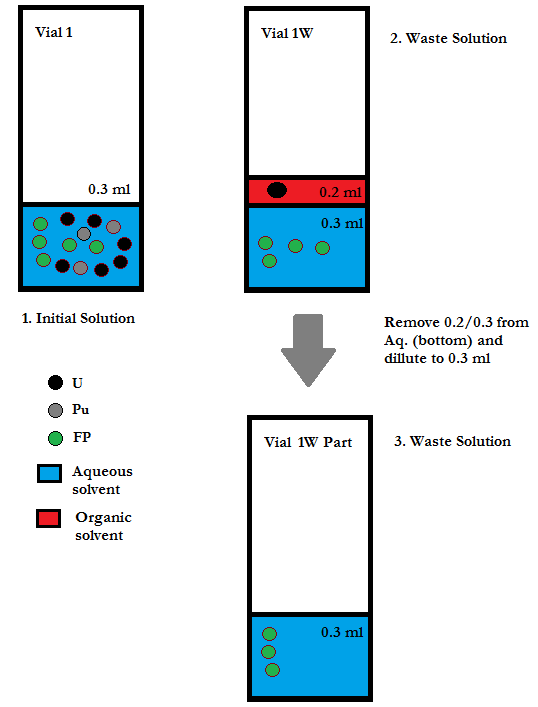
\includegraphics[width=0.5\linewidth]
                  {Figures/Extraction_Process_1_First_3_Counts}
\end{center}
\caption{First Three Counts}
\label{fig:example1}
\end{figure}

\begin{figure}[H] % Example of including images
\begin{center}
  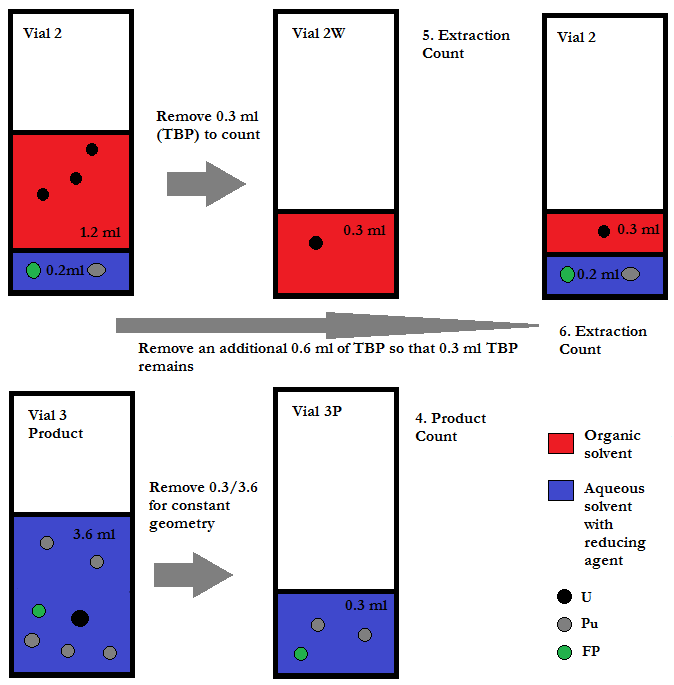
\includegraphics[width=0.5\linewidth]
                  {Figures/Back_Extraction_Process_1_Last_3_Counts}
\end{center}
\caption{Second Three Counts}
\label{fig:example2}
\end{figure}

%------------------------------------------------------------------------
%	LAB BOOK day
%-----------------------------------------------------------------------

\labday{Wednesday, 12 October 2016\\ 11:30 am - 1:30 pm}

\experiment{Process1_Fail_Counting}

\begin{todolist}
\item[\done]{Finish count $\boxed{3P}$}
\item[\done]{Start sample $\boxed{2W}$}
\item[\done]{Determine preliminary results}
  \begin{itemize}
  \item{Determined \tss{137}Cs, \tss{144}Ce, \tss{106}Rh
    activities for first 4 counts - Excel sheet}
  \item{Used excel sheet from John Burns for efficiency
    calibration of Eu-152 source...will just use
    the sheet from now on}
  \item{Also got from John, a templating file for GENIE,
    ``AnalysisMG.tpi'', which helps a lot for output from
    GENIE, again, something I do not want to modify}
  \item{The template was in an algorithm from GENIE, had
    the following steps}
    \begin{enumerate}
    \item{Peak Locate - Unidentified 2nd Diff}
      \begin{itemize}
      \item{Channels 1-16000}
      \item{2.50}
      \item{0.50 - FWHM}
      \item{Add to existing results}
      \end{itemize}
    \item{Peak Area - Sum/Non-linear LSQ Fit}
      \begin{itemize}
      \item{Channels 1-16000}
      \item{4 channels, use fixed tail parameters}
      \item{Channels, Step, 4.00, 4.00, 4.00}
      \item{Output to screen and printer}
      \end{itemize}
    \item{Reporting...}
      \begin{itemize}
      \item{``AnalysisMG.tpi'', ``C:/GENIE2K/CTLFILES/''}
      \item{PeakAnalysis, 1.000000}
      \item{Start on: Page One, New File, $\mu$Ci}
      \end{itemize}
    \end{enumerate}
  \end{itemize}
\item[\done]{Notes for research meeting}
  \begin{itemize}
  \item{Process dilutes by factor of 12, no matter what}
  \item{Concentrated stock by a factor of two}
  \item{Decreased initial volume}
  \item{Have to mainatin, 0.2 ml excess volume to pipette from top}
  \item{Have to maintain, 0.1 ml excess from bottom}
  \item{Mistake in extraction - all extractions at once}
  \end{itemize}
\end{todolist}



%------------------------------------------------------------------------
%	LAB BOOK day
%-----------------------------------------------------------------------

\labday{Thursday, 13 October 2016\\ 12:30 am - 4:30 pm}

\experiment{Process1_Fail_Counting}

\begin{todolist}
\item[\done]{Finish count $\boxed{2W}$}
\end{todolist}

\experiment{Process1_Fail_Counting2}
\begin{todolist}
\item[\done]{Start count $\boxed{2}$}
\item[\done]{Fix alpha counter, reivew alpha counting}
  \begin{itemize}
  \item{Alpha detector broken, fixed by plugging into proper port}
  \item{Counted Calibration Alpha source}
    \begin{itemize}
    \item{There are some details for determining
      what the alpha efficiency should be for the alpha
      detector, and I want to make sure I do it correctly,
      have not had time to look into it. I have a PDF file
      that shows what is in the sample\\
      /notebook/Figures/Alpha\_Copy.pdf}
    \item{Pu-239 and Pu-240 are unresolved}
    \item{Pu-238 and Am-241 are unresolved}
    \item{Isotope Droduets Laboratories}
    \item{38.81 nCi}
    \item{1451-68-3}
    \item{1 Dec 10}
    \item{Kevin also provided me with a Excel Sheet that does
      some of the calculations, probably will have to modify}
    \end{itemize}
  \end{itemize}
\item[\done]{Counted Alpha Background}
\item[\done]{Counted Alpha Calibration (9 mm position)}
\item[\done]{Prepare alpha sample of $\boxed{Stock}$}
  \begin{itemize}
    \item{From Jarrod's stock 10$\mu$l was diluted to 1ml
    and 10 $\mu$l was taken}
  \end{itemize}
\end{todolist}
\begin{center}
10 $\mu$l of $\boxed{Stock}$ (4 M HNO\tsbs{3})\\
+\\
\st{190 $\mu$l of DI water (leftover in glovebox)}\\
990 $\mu$l of DI water (leftover in glovebox)\\
=\\
\st{0.2 ml of $\sim$ 0 M HNO}\tsbs{3}\st{ $\boxed{4\ Dilution}$}\\
1 ml of $\sim$ 0 M HNO\tsbs{3} $\rightarrow\boxed{4\ Dilution}$
\end{center}
\begin{todolist}
\item[\done]{Prepare and count alpha sample of Stock}
  \begin{itemize}
  \item{Take 20 $\mu$l of $\boxed{4\ Dilution}$, put onto
  concentric circle disk plates (innermost circle) $\boxed{D1}$}
    \begin{itemize}
    \item{It should be noted that once an alpha source is
      placed on these disks and dried out, they look no different
      from other disks}
    \end{itemize}
  \item{Let dry in glovebox}
  \end{itemize}
\item[\done]{Count $\boxed{D1}$ over night}
\end{todolist}

%------------------------------------------------------------------------
%	LAB BOOK day
%-----------------------------------------------------------------------

\labday{Friday, 14 October 2016\\ 8:30 am - 9:00 pm}

\experiment{Process1_Fail_Counting}

\begin{todolist}
\item[\done]{Finish count $\boxed{2}$}
\end{todolist}

\experiment{Process1_Fail_Counting2}
\begin{todolist}
\item[\done]{Finish count for $\boxed{D1}$}
\item[\done]{Move $\boxed{D1}$ to safe (or glovebox)}
\end{todolist}

\experiment{Process1_Fail_Counting_Analysis}
\begin{todolist}
\item{Attempt to understand our alpha efficiency (basically
  how much is in the calibration source)}
\end{todolist}

%------------------------------------------------------------------------
%	LAB BOOK day
%-----------------------------------------------------------------------

\labday{Monday - Wednesday, 17-19 October 2016}

\experiment{Process1_Fail_Counting_Analysis}

\begin{todolist}
\item{Looked into alpha calibration math some more}
\item[\done]{Analyze and automate (somewhat) Gamma analysis}
  \begin{itemize}
  \item{Program for pulling peak data from GENIE}
  \item{Program for calculating efficency from peak energy data using
    John Burn's Excel file}
  \item{Determine Compton Edges for peaks}
    \begin{itemize}
    \item{$$E_f=\frac{E_i}{1+\frac{E_i}{511}(1-cos\theta)}$$}
    \item{$$E_i=\frac{E_f}{1-\frac{E_f}{511}(1-cos\theta)}$$}
    \item{Found that I do not have any back scatter peaks}
    \end{itemize}
  \item{Program for finding sum peaks}
    \begin{itemize}
    \item{Included backscatter peaks}
    \item{Found some coincidence peaks, didn't know how to analyze}
    \end{itemize}
  \item{Quantify most of the peaks in gamma spectrum (took the longest)}
    \begin{itemize}
    \item{$$CPS=A\gamma\epsilon$$}
    \item{$$CPS=A_1\gamma_1\epsilon_1+A_2\gamma_2\epsilon_2$$}
    \item{Most peaks used the first equation, one peak had
      overlapping energies, so used the second equation,
      had to assume one of the activities}
    \end{itemize}
  \item{Applied this analysis to
    6 gamma spectrum (took second longest - now more automated)}
  \item{Create graphics to help depict
    what work was actually done}
  \end{itemize}
\item[\done]{Note: Follow these steps when analyzing Gamma}
  \begin{enumerate}
  \item{Make sure Efficiency Excel Sheet is up to date}
    \begin{itemize}
    \item{Run Eff Count and particular distance}
    \item{Run: ``Analyze - Execute Sequence - Analyze\_Data''
      on GENIE}
    \item{Save as a .PDF (not .pdf) file the spectra data
      : File - Export Report to PDF from GENIE}
    \item{Pull Peak information with Data\_Pull.py program (direct
    program to directory with .PDF file)}
    \item{Put data into spreed sheet
    ``C:/Rad\_Detection/Calibration/Gamma/Eff\_cal\_summary\_Eu-152.xlsm''}
    \end{itemize}
  \item{Gather data in a similar manner as with the efficiency count
  - will produce a bunch of plain Excel Sheets}
  \item{Find the template  from C:/Rad\_Dection folder, update
    real Eff column with ``Eff\_Calc.py'' (Make sure you
    copy paste energies into the gamma\_energies file)}
  \item{Copy this template over to the sheets you just made,
    and gamma analysis for the peaks will be complete}
    \begin{itemize}
    \item{Note: Will have to copy, paste, remove peak columns that
      were not found or in excess from template, lining up everything
      and then delete was copied over, then paste again, janky,
      but not super slow - this list is a reminder for Paul,
      if anyone else is using this list, would probably need
      more explanation }
    \end{itemize}
  \end{enumerate}
\item[\done]{Notes for Research Meeting}
  \begin{itemize}
  \item{Showed activities for each of the solutions}
  \item{Found that D-values couldn't be found because
    of experimental setup}
  \item{Activity Balance seemed to match up}
    \begin{itemize}
    \item{Although it wasn't perfect because the numbers
    weren't exactly close to zero, but within the error}
    \end{itemize}
  \item{Results seemed to match up with previous experiment}
  \item{Moving Forward, John and Sunil and I discussed
    what these next experiments should entail}
  \end{itemize}
\end{todolist}


%------------------------------------------------------------------------
%	LAB BOOK day
%-----------------------------------------------------------------------

\labday{Thursday, 20 October 2016}

\experiment{Cycle_X3_Prep}

Note from John:\\~\\
After the research meeting yesterday, I thought about Paul’s
project quite a bit and what the best path forward should be.
\textbf{In my opinion, it would be best for him to do a single-cycle}
\textbf{(extraction/back extraction) in a replicate of 3 and determine}
\textbf{the D-values for both the extraction and back extraction and}
\textbf{show the reproducibility of this single-cycle experiment.} I
believe this is one of the goal you set for him as a part of
his proposal. From there we can move into the whole process
with confidence that we have consistent behavior for Cs-137
and Cs-134, as well as, a good understanding of the D-values
for the isotopes of interest that can be seen by gamma-ray
analysis. He and I spent some time this morning talking about
this and we both agree that this week he will focus on completing
all 3 single-cycle replicates, gamma counting all the solutions,
alpha counting as many as possible (I do not believe alpha and
gamma counts cannot be performed at the same time, as they both
use the computer), and analyzing a majority of the data before
next week’s research meeting. If you do not think this is plan
of action in the best to pursue we can restructure it.
\\~\\
I spend the rest of the day doing homework, I aplogize,
but it was due yesterday, I think its dumb that I should
have to apologize for spending \textbf{ANY} time doing homework.
\\~\\
John also mentioned two good techniques, that should be noted:
\begin{itemize}
\item{Pipetting with equal volumes using the plastic squish tops}
  \begin{itemize}
  \item{Squeeze top while going through organic, suck up as much as
    possible}
  \item{Then draw from top as well}
  \end{itemize}
\item{Measureing volume with pipette}
  \begin{itemize}
  \item{The above technique would need some means for measuring volume
    using the pipette, you can vary the volume around
    what you thought you sucked up, and check if there is air
    at the bottom of the tip}
  \end{itemize}
\end{itemize}


%------------------------------------------------------------------------
%	LAB BOOK day
%-----------------------------------------------------------------------

\labday{Friday, 21 October 2016\\ 9:30am - 12:00 pm\\1:00 pm 6:00 pm}

\begin{todolist}
\item[\done]{Updated this lab notebook (most of this morning)}
\end{todolist}

\experiment{Cycle_X3_Prep}

\begin{todolist}
\item[\done]{Practice pipetting out with squish tops like John Mentioned}
  \begin{itemize}
  \item{Used Kerosene solution, used squish pipettes and variable
    pipettes - settled upon using 500 $\mu$l
    and taking out 350 $\mu$l and then
    getting as much out as possible with the squish pipette -
    I get about 450 $\mu$l of bottom phase (HNO\tsbs{3})
    and 425 $\mu$l of top phase (TBP)}
  \item{Determine if 0.3 ml is a good amount of solution to use}
  \item{Switching to 0.5 ml, keeping smaller vials}
  \end{itemize}
\item[\done]{Create and label vials $\boxed{5}$ $\boxed{6}$ and
  $\boxed{7}$ to hold stock solution. Did not leech them,
  hopefully barium contamination wont be a huge deal,
  we will assume all the data for Cs can be gathered from \tss{133}Cs.}
\item[\done]{Transfer 0.5 ml of $\boxed{Stock}$ to $\boxed{5}$}
\item[\done]{Transfer 0.5 ml of $\boxed{Stock}$ to $\boxed{6}$}
\item[\done]{Transfer 0.5 ml of $\boxed{Stock}$ to $\boxed{7}$}
\item[\done]{Add scoop of sodium nitrite to $\boxed{5}$}
\item[\done]{Add scoop of sodium nitrite to $\boxed{6}$}
\item[\done]{Add scoop of sodium nitrite to $\boxed{7}$}
\item[\done]{Centrifuged $\boxed{5}$, $\boxed{6}$
  and $\boxed{7}$ to push all solution to
  botttom of vials}
\item[\done]{Start count of $\boxed{5}$ noticed bubbles in solution,
  might have to recount - left overnight}
\end{todolist}

\experiment{Process1_Fail_Counting2}

\begin{todolist}
\item[\done]{Took 20 $\mu$l out of $\boxed{3}$ and put
  onto planchet chip (no dilution)}
  \begin{itemize}
  \item{Moved chip too early (before drying, ruined
    detector volume)}
  \item{Made another source with an additional 20 $\mu$l,
    letting it dry over night}
  \end{itemize}
\end{todolist}



%------------------------------------------------------------------------
%	LAB BOOK day
%-----------------------------------------------------------------------

\labday{Saturday, 22 October 2016\\ 3:30 pm - 3:45 pm\\ 8:00 pm - 8:30 pm}

\experiment{Cycle_X3_Prep}

\begin{todolist}
\item[\done]{Finished count for $\boxed{5}$}
\item[\done]{Started count of $\boxed{6}$}
  \begin{itemize}
  \item{Switching from push clear caps to blue push caps}
  \item{This sample had less bubbles than the one yesterday}
  \end{itemize}
\item[\done]{Finished count of $\boxed{6}$}
  \begin{itemize}
  \item{Some liquid was not at the bottom of the vial,
    messing with geometry, centrifuged with $\boxed{7}$
    might have to recount}
  \end{itemize}
\item[\done]{Started count of $\boxed{7}$}
  
\end{todolist}

%------------------------------------------------------------------------
%	LAB BOOK day
%-----------------------------------------------------------------------

\labday{Sunday, 23 October 2016}

\experiment{Cycle_X3_Prep}

\begin{todolist}
\item[\done]{Finished count $\boxed{7}$}
\item[\done]{Analyzed Counts from $\boxed{5}$, $\boxed{6}$, and
  $\boxed{7}$}
  \begin{itemize}
  \item{Did not like how $\boxed{6}$ didn't fit with others}
  \end{itemize}
\item[\done]{Started recount of $\boxed{6}$}
\item[\done]{Start Excel Sheet for analysis and
           write program for quicker gamma analysis}
\end{todolist}

%------------------------------------------------------------------------
%	LAB BOOK day
%-----------------------------------------------------------------------

\labday{Monday, 24 October 2016\\10:00 am - 12:00 pm\\3:00 pm -
        8:00 pm}

\experiment{Cycle_X3_Prep}

\begin{todolist}
\item[\done]{Finished count $\boxed{6}$}
\item[\done]{Transfer:}
  \begin{itemize}
  \item{Vials labeled $\boxed{5\ Aq}$, 
    $\boxed{5\ Or}$, $\boxed{6\ Aq}$, $\boxed{6\ Or}$,
    $\boxed{7\ Aq}$, $\boxed{7\ Or}$}
  \item{With clear push lids, and blue push lids (named)}
  \item{Squish pipettes}
  \end{itemize}
  Into glovebox small antichamber
\item[\done]{$\boxed{5}$, $\boxed{6}$, and $\boxed{7}$ already
  in antichamber}
\item[\done]{Transfer vials with clear lids into glovebox, but
  leave the blue lids in the antichamber (lid transfer area)}
\item[\done]{Dump $\boxed{Back\ Ex\ Solution}$ into aqeuous
  waste ($\sim$ 0.2 $\mu$l) (decays - will prepare a fresh batch)}
\end{todolist}

\experiment{Process1_Fail_Counting2}

\begin{todolist}
\item[\done]{Moved alpha sample to count on PIPS detector}
  \begin{itemize}
  \item{Saw energy smearing for counts}
  \item{Preliminary results are what was expected if
    we take a larger range of counts}
  \end{itemize}
\end{todolist}

\experiment{Cycle_X3}

\begin{todolist}
\item[\done]{Add 500$\mu$l TBP to $\boxed{5}$, $\boxed{6}$,
  $\boxed{7}$}
\item[\done]{Shake $\boxed{5}$ on Pulse mode for 15 minutes}
\item[\done]{Shake $\boxed{6}$ on Pulse mode for 15 minutes}
\item[\done]{Shake $\boxed{7}$ on Pulse mode for 15 minutes}
\item[\done]{Create $\boxed{EX Buddy}$ so all samples can be
  centrifuged together}
  \begin{itemize}
  \item{500 $\mu$l of 4 M HNO\tsbs{3} + 500 $\mu$l of 30 vol.\%
    TBP}
  \end{itemize}
\item[\done]{Centrifuge samples for 3000 rpm for 5 minutes}
\item[\done]{Separate phases for samples}
  \begin{itemize}
  \item{A total of 4 drops were dropped in this process}
    \begin{enumerate}
    \item{Sample $\boxed{5}$ aqueous transfer}
    \item{Sample $\boxed{6}$ organic transfer}
    \item{Sample $\boxed{7}$ aqueous and organic transfer}
    \end{enumerate}
  \item{Using a variable pipette and the squish pipette,
    as much of the top phase (organic) phase was removed as possible
    (turns out to be around 450 $\mu$l and transfered to
    $\boxed{5\ Or}$, $\boxed{6\ Or}$, and $\boxed{7\ Or}$.}
  \item{Then as much of the bottom phase (aqueous) was removed as
    possible (turns out to be around 430 $\mu$l) and transfered
    to $\boxed{5\ Aq}$, $\boxed{6\ Aq}$, and $\boxed{7\ Aq}$.}
  \end{itemize}
\item[\done]{Measure Volumes of 9 vials (Aqueous, organic, and original
  - units of $\mu$l)}
  \begin{itemize}
  \item{Clean outside of vials before taking volume measurements}
  \item{Centrifuge vials before taking volume measurements}
  \item{Google says that 1 drop of water is about 50 $\mu$l}
  \end{itemize}
\end{todolist}
\begin{center}
  \begin{tabular}{||c c c c c c||}
    \hline
    Series & Aqueous & Organic & Original & Should Add To & Missing\\ [0.5ex]
    \hline\hline
    5 & 461+/-9.22 & 430+/-8.6 & 55+/-5 & 1000+/-7.1 & 54+/-15.3\\
    \hline
    6 & 469+/-9.38 & 430+/-8.6 & 53+/-5 & 1000+/-7.1 & 48+/-15.4\\
    \hline
    7 & 469+/-9.38 & 430+/-8.6 & 57.5+/-5 & 1000+/-7.1 & 43.5+/-15.4\\
    \hline
  \end{tabular}
\end{center}

\begin{todolist}
\item[\done]{Count $\boxed{7\ Or}$ 12:00 pm - 6:00 pm}
\item[\done]{Start count $\boxed{7\ Or}$ on face of detector 6:00 pm
  this is because I cannot see \tss{134}Cs - the isotope I am
  most concerned about}
  \begin{itemize}
  \item{Will try and implement this:}
    $$CPS=A\epsilon_D\epsilon_G\gamma$$
    Where:
    \begin{center}
    $\epsilon_D=$Detector eff\\
    $\epsilon_G=$Geometric eff\\
    $\gamma=$yield\\
      $A=$activity
    \end{center}
    At two different distances $1$ and $2$:
    \begin{align*}
      CPS_1&=A\epsilon_D\epsilon_{G1}\gamma\\
      CPS_2&=A\epsilon_D\epsilon_{G2}\gamma
    \end{align*}
    Take ratio:
    \begin{equation*}
      \frac{CPS_1}{CPS_2}=\frac{A\epsilon_D\epsilon_{G1}\gamma}
           {A\epsilon_D\epsilon_{G2}\gamma}=
           \frac{\epsilon_D\epsilon_{G1}}{\epsilon_D\epsilon_{G2}}
           =R
    \end{equation*}
    Kept both efficiencies because calibration lumps both together.
    If This ratio, $R$ is known, then we can count at a closer
    distance and say:
    \begin{equation*}
      CPS_2=\frac{CPS_1}{R}
    \end{equation*}
  \end{itemize}
\item[\done]{Move $\boxed{6\ Or}$ and $\boxed{7\ Aq}$ to Antichamber
  (not sure which one I am counting next)}
\end{todolist}

\experiment{programs}
\begin{todolist}
\item[\done]{Modify program for analyzing spectra}
  \begin{itemize}
  \item{Hopefully now analyzing gamma data will just be,
    run program, and copy a part of an excel spreedsheet}
  \end{itemize}
\end{todolist}

%------------------------------------------------------------------------
%	LAB BOOK day
%-----------------------------------------------------------------------

\labday{Tuesday, 25 October 2016\\8:00 am}


\experiment{Cycle_X3}


\begin{todolist}
\item[\done]{Count $\boxed{6\ Or}$ 8:00 pm - 11:00 am}
\end{todolist}

\experiment{Contamination}
\begin{todolist}
\item{\st{Go to count $\boxed{5\ Or}$}}
  \begin{itemize}
  \item{Have $\boxed{7\ Or}$ and $\boxed{7\ Aq}$ in small
    antichamber}
  \item{Put antichamber to vacuum to transfer vials into
    glovebox}
  \item{Push caps exploded off vials due to large pressure
    difference...that is very dissapointing}
  \end{itemize}
\item[\done]{Clean up contamination from exploded vials in antichamber}
  \begin{itemize}
  \item{Dispose of counting vials, and caps for all vials rad waste}
  \item{Dispose of exploded vials in rad waste (after dried)}
  \item{Remove diaper paper from transfer plate}
  \item{Clean with radiac wipes}
    \begin{itemize}
    \item{Clean antichamber}
    \item{Clean antichamber}
    \item{Swipe area, count on alpha detector, because
      our swipe counter is down}
    \item{Clean antichamber}
    \item{Dr. Chirayath brought someone by to talk, not a good time}
    \item{Clean antichamber}
    \item{Clean glass beaker that was in antichamber...lots}
    \end{itemize}
  \item{Final areas swiped and counted for 10
    minutes after decontamination}
    \begin{itemize}
    \item{Tray $\sim$0 counts in alpha realm}
    \item{Top part of cylinder of antichamber
      $\sim$3 counts in alpha realm (around 20 for background)}
    \item{Top back part of cylinder $\sim$ 100 - still slightly
      contaminated, but no time for continued cleaning,
      because need to do experiment}
    \item{Left/Right side of cylinder (mid plane) $\sim$ small}
    \item{Bottom back portion of cylinder of antichamber - $\sim$100}
    \item{Glass vial - none}
    \end{itemize}
  \end{itemize}
\end{todolist}
\experiment{Cycle_X3}
\begin{todolist}
\item[\done]{Count $\boxed{5\ Or}$ 3:00 pm - 7:30 pm (finally!!)}
\item{\st{Count $\boxed{7\ Aq}$ 9:00 pm - 11:00 pm} (Spilled)}
\item[\done]{Count $\boxed{6\ Aq}$ 7:00 pm - 9:00 pm}
\item[\done]{Count $\boxed{5\ Aq}$ 9:00 pm - 8:00 am}
\end{todolist}
\begin{todolist}
\item[\done]{-}
\end{todolist}
\begin{center}
0.0417+/-0.0018 ml of 2.302+/-0.009 M Fe(II) in 0.0+/-0 M HNO\tsbs{3} $\boxed{Stock\ Fe(II)}$\\
+\\
3.941+/-0.027 ml of 0.0+/-0 M Fe(II) in 4.06+/-0.05 M HNO\tsbs{3} solution $\boxed{Fe\ Prep}$\\
+\\
4.000+/-0.020 ml of 0.0240+/-0.0010 M Fe(II) in 4.00+/-0.05 M HNO\tsbs{3} solution $\boxed{\rightarrow Bk\ Ex\ Solution}$.
\end{center}
\begin{todolist}
\item[\done]{Add 430 $\mu$l Fe(II) solution to $\boxed{5\ Or}$}
\item[\done]{Add 430 $\mu$l Fe(II) solution to $\boxed{6\ Or}$}
\item{\st{Add XX $\mu$l Fe(II) solution to $\boxed{7\ Or}$} (spilled)}
\item[\done]{Shake $\boxed{5\ Or}$ 15 minutes on pulse mode}
\item[\done]{Shake $\boxed{6\ Or}$ 15 minutes on pulse mode}
\item{\st{Shake $\boxed{7\ Or}$ 15 minutes on pulse mode} (spilled)}
\item{\st{Remove XX $\mu$l organic and XX $\mu$l aqueous
  from $\boxed{Ex\ Buddy}$} (No longer necessary)}
\item[\done]{Centrifuge $\boxed{5\ Or}$, $\boxed{6\ Or}$, \st{$\boxed{7\ Or}$}
  \st{$\boxed{Ex\ Buddy}$}, 3,000 rpm for 5 minutes}
\end{todolist}
\begin{todolist}
\item[\done]{Vials labeled $\boxed{5\ AqII}$, 
  $\boxed{5\ OrII}$, $\boxed{6\ AqII}$, $\boxed{6\ OrII}$,
  \st{$\boxed{7\ AqII}$, $\boxed{7\ OrII}$}, transfered into
  glovebox}
\item[\done]{Separate phases for samples}
  \begin{itemize}
  \item{A total of 1 drops were dropped in this process}
    \begin{enumerate}
    \item{Sample $\boxed{5\ Or}$ aqueous or organic transfer}
    \end{enumerate}
  \item{Using a variable pipette and the squish pipette,
    as much of the bottom phase (aqueous) phase was removed as possible
    and transfered to
    $\boxed{5\ OrII}$, $\boxed{6\ OrII}$, and \st{$\boxed{7\ OrII}$}.}
  \item{Then as much of the top phase (organic) was removed as
    possible and transfered
    to $\boxed{5\ AqII}$, $\boxed{6\ AqII}$, and \st{$\boxed{7\ AqII}$}.}
  \end{itemize}
\item[\done]{Measure Volumes of 9 vials (Aqueous, organic, and original
  - units in $\mu$l)}
\end{todolist}
\begin{center}
  \begin{tabular}{||c c c c c c||}
    \hline
    Series & Aqueous II & Organic II & Original II & Should Add to
    & Missing\\ [0.5ex]
    \hline\hline
    5 & 407+/-8.14 & 380+/-7.6 & 38+/-5 & 860+/-12.2 & 35.0+/-17.2\\
    \hline
    6 & \st{402}415+/-8.3 & \st{360}380+/-7.6 & 35+/-5 & 860+/-12.2
    & 30+/-17.3\\
    \hline
  \end{tabular}
\end{center}

\experiment{programs}

\begin{todolist}
\item[\done]{Updated Spreedsheets to calculate
  activities based on avaiable peaks, also if
  a particular peak has really large errors,
  this will be ignored. Also updated Excel sheets
  to calculate propagated error mass in each vial
  - for D-value calculations}
  \begin{equation*}
    grams=\frac{\text{Activity}\times\text{Molar Mass}}
    {\lambda_sN_A}
  \end{equation*}
  where $\lambda$ is in seconds and $N_A$ is avogadros number.
\end{todolist}


 
%------------------------------------------------------------------------
%	LAB BOOK day
%-----------------------------------------------------------------------

\labday{Wednesday, 26 October 2016\\8:00 am}


\experiment{Cycle_X3}

\begin{todolist}
\item[\done]{Finish count $\boxed{5\ Aq}$}
\item[\done]{Start count $\boxed{6\ AqII}$}
\item[\done]{Analyze current spectra}
  \begin{itemize}
  \item{Calculate activity (with error) for
    vials $\boxed{5}$, $\boxed{6}$, $\boxed{7}$,
    $\boxed{5\ A}$, $\boxed{5\ O}$, $\boxed{6\ A}$,
    $\boxed{6\ O}$, $\boxed{7\ O}$}
  \item{Calculate, for those same vials (with error,
    even including error on molar mass), mass of each
    radioactive species, and the concentration (g/L)}
  \item{Compared all first solution activities and concentrations,
    they were all very similar}
  \item{Compared \tss{137}Cs \tss{134}Cs ratio, and they agreed between
    vials}
  \item{Determined activity balance, making sure each
    cycle had balance of activity (measured a part of the solution
    459/500, found grams per liter, and multiplied by 400).}
    \begin{itemize}
    \item{Agreed within the error}
    \end{itemize}
  \item{Determined D-values from aqueous and organic solutions,
    compared same elements different isotopes}
    \begin{itemize}
    \item{The numbers did not look super similar,
      but sort of similar}
      \begin{equation*}
        O\%=\frac{1}{1+\frac{V_{A}}{V_{O}D}}
        \Rightarrow D_O=\frac{1}{\frac{V_O}{V_A}(\frac{1}{O\%}-1)}
      \end{equation*}
      \begin{equation*}
        A\%=\frac{1}{1+\frac{V_OD}{V_A}}\Rightarrow
        D_A=\frac{V_A}{V_O}(\frac{1}{A\%}-1)
      \end{equation*}
      Where O and A represent organic and aqueous, where
      V is volume and \% refers to mass percent in a
      particular phase.
      The mass percent was determined via:
      \begin{equation*}
        \%=\frac{\text{Mass Part}}{\text{Total Mass}}=
        \frac{c\ \left[\frac{g}{L}\right]\cdot V_{\text{contact}}}
        {\text{Mass in original}}
      \end{equation*}
    \end{itemize}
  \item{Propagate error for D-value calculation (as well as for others)}
    \begin{itemize}
    \item{Attempted to install uncertainties onto python
      on windows system, but failed epically, windows is terrible}
    \item{Instead used uncertainties on linux based system to check
      my answers for the below codes}
      \begin{center}
        Aqueous D-value calculation
      \end{center}
      \begin{equation*}
        \sigma_{D_A}^2=\left[\frac{ \sigma_{V_A} }{V_O}
          \left(\frac{1}{A\%}-1\right)
          \right]^2+\left[\frac{V_A\sigma_{V_O}}{V_O^2}
          \left(\frac{1}{A\%}-1\right)
          \right]^2+\left[\frac{V_A\sigma_{A\%}}{V_OA\%^2}\right]^2
      \end{equation*}
      \begin{center}
        Organic D-value calculation
      \end{center}
      \begin{equation*}
        \sigma_{D_O}=\sqrt{
          \left[\frac{ \sigma_{V_O} }{V_A}
          \left(\frac{1}{O\%}-1\right)
          \right]^2+\left[\frac{V_O\sigma_{V_A}}{V_A^2}
          \left(\frac{1}{O\%}-1\right)
          \right]^2+\left[\frac{V_O\sigma_{O\%}}{V_AO\%^2}\right]^2
          }\cdot D_O^2
      \end{equation*}
    \end{itemize}
  \end{itemize}
\item[\done]{Create graphic to explain these results to
  research group}
\end{todolist}

\experiment{Contamination}
\begin{todolist}
\item[\done]{Create graphic of all alpha spectra and locations of swipes}
\item[\done]{Called EHS, talked to Dan Manchaka about contamination
  spill yesterday}
  \begin{itemize}
  \item{d-imenchaca@tamu.edu}
  \item{979-676-0590}
  \end{itemize}
\item[\done]{EHS came by $\sim$3:20pm to evaluate the contamination
  in the lab}
  \begin{itemize}
  \item{Asked about the incident - reported}
  \item{Took pictures of glovebox and room}
  \item{Swiped and surveyed}
  \end{itemize}
\end{todolist}

\experiment{ResearchMeeting}
\begin{itemize}
\item{Note that Dr. Chirayath needs a VGA to HDMI converter}
\item{Discussed research results}
  \begin{itemize}
  \item{Want the third experiment to be completed}
  \end{itemize}
\item{Discussed contaminaiton}
  \begin{itemize}
  \item{Specific Activity of \tss{239}Pu: 0.063 $\frac{Ci}{g}$,
        largest amount of Pu released: 5 $\mu$g}
    \begin{align*}
      0.063\frac{Ci}{g}\cdot\frac{10^{-6}g}{\mu g}
      \cdot \frac{3.7\times10^{10}Bq}{Ci}=&2331
      \frac{Bq}{\mu g}\\
      &2331\cdot5\mu g=11655Bq
    \end{align*}
  \item{Specific Activity of \tss{238}U: 12,445 $\frac{Bq}{g}$,
    largest amount of U released: \\0.000258 g}
    \begin{align*}
      0.000258\ g\cdot12445\frac{Bq}{g}=3.21 Bq
    \end{align*}
  \end{itemize}
\item{Annual intake limits $\sim$300 Bq}
\item{Say 40\% was released to air: 4663 Bq}
\item{Room size is about 72 cubic meters = 72000 liters}
\item{0.065 Bq/liter}
\item{Human breathes 20 times per minute with 6 liter capacity}
\item{2 liters per second, 7200 liters per hour}
  \begin{equation*}
    0.065\frac{Bq}{liter}\cdot7200\frac{liters}{Hr}=
  468 \frac{Bq}{Hr}
  \end{equation*}
\item{Things to discuss with Dan:}
  \begin{enumerate}
  \item{Ask Dan if a spill procedure should exist for
    antichamber}
  \item{Remind Dan biggest concern is evaporation}
  \item{Should we get Masks}
  \end{enumerate}
\end{itemize}

 
%------------------------------------------------------------------------
%	LAB BOOK day
%-----------------------------------------------------------------------

\labday{Thursday, 27 October 2016\\9:30 am}

\begin{todolist}
\item[\done]{Update laboratory notebook}
\item{Determine calculation for alpha samples}
\item{Outline project for UQ}
\item[\done]{Meet with Dan Menchaka about rad stuff}
  \begin{itemize}
  \item{Called him on the phone}
  \item{He said that swipes came back clean}
  \item{That I could continue to decontaminate in the glovebox}
  \end{itemize}
\item[\done]{Installed uncertainties on windows computer}
  \begin{itemize}
  \item{Go to start menu}
  \item{cmd, run in administrator mode}
  \item{type\_path\_to\_pip install package}
  \end{itemize}
\item[\done]{Automated copy paste from Gamma\_Template to excel
  sheet}
\end{todolist}

\experiment{Cycle_X3}

\begin{todolist}
\item[\done]{Finish counting $\boxed{6\ AqII}$}
\item[\done]{Start counting $\boxed{5\ AqII}$}
\end{todolist}

%------------------------------------------------------------------------
%	LAB BOOK day
%-----------------------------------------------------------------------

\labday{Friday, 28 October 2016}

\experiment{Contamination}

\begin{todolist}
\item[\done]{Clean contamination in glovebox}
  \begin{itemize}
  \item{Swipe L Shoe - clean}
  \item{Swipe R Shoe - clean}
  \item{Swipe Top    - clean}
  \item{Swipe Left Right Mid plane - clean}
  \item{Swipe around the top back portion - clean}
  \item{Swipe Back bottom - clean}
  \end{itemize}
\end{todolist}

\experiment{Cycle_X3}

\begin{todolist}
\item[\done]{Finish count $\boxed{5\ AqII}$}
\item[\done]{Checked math with John Burns}
  \begin{itemize}
  \item{The math was correct, but we noticed that
    Series 6 had larger D-values accros the board}
  \item{If we assume a 10 $\mu$l contamination
    of aqueous in the organic (a very small amount),
    the D-values line up a lot better}
    \begin{itemize}
    \item{Eu-155 0.07 to 0.049 \done}
    \item{Eu-155 0.09 to 0.073 \wontfix}
    \item{Eu-154 0.095 to 0.073 \wontfix}
    \item{Ce-144 0.045 to 0.022 \done}
    \item{Rh     0.067 to 0.045 \done}
    \item{Cs-137 0.024 to 0.001 \done}
    \end{itemize}
  \end{itemize}
\item[\done]{Start background count}
\item[\done]{Go home, not feeling well}
\end{todolist}


%------------------------------------------------------------------------
%	LAB BOOK day
%-----------------------------------------------------------------------

\labday{Monday, 31 October 2016}

\experiment{Cycle_X3}
\begin{todolist}
\item[\done]{Start Efficiency Count with Eu-152 Liquid source}
\item[\done]{Stop Efficiency count once contamination was found
  need to clean HPGe}
\end{todolist}

\experiment{Contamination}
\begin{todolist}
\item[\done]{Luis Gonzolas and Daniel Menchaca both came by around
  10:00 am to take swipes around the antechamber}
  \begin{itemize}
  \item{They said they would get results after lunch}
  \end{itemize}
\item[\done]{Write up small report about contamination leak
  and give to Latha, in subdirectory ``Indicent''}
  \begin{itemize}
  \item{Assumed 90\% of the 7 series in the antechamber, and the
    other 10\% is in the original 7 vial that wasn't spilled}
  \end{itemize}
\end{todolist}

\experiment{Contamination2}

\begin{todolist}
\item[\done]{Clean HPGe, reduce background contamination}
  \begin{itemize}
  \item{Clean all bricks}
  \item{Count with bricks in different configurations}
  \item{Found that source is coming from radiation storage closet}
  \end{itemize}
\item[\done]{Ask Troy if he moved sources around in closet,
  or if anyone did}
  \begin{itemize}
  \item{He did say that someone moved stuff around}
  \item{Shielded our source (probably strongest source around)}
  \end{itemize}
\item[\done]{Recount background, still high on Cs-137 source...}
\item[\done]{Ask Marianno for doubloon reward...and if he aquired
  any sources recently, he said he did, he got 1.3 or so mCi of
  \tss{137}Cs...that would explain it, I asked which day
  he got the source, to know when to subtract out the background
  from my samples...he said he would check}
\item[\done]{This took a large portion of the day}
\end{todolist}

\begin{center}
  Dig around the roots\\
  Grace and Truth \\
  Next season will come
\end{center}

%------------------------------------------------------------------------
%	LAB BOOK day
%-----------------------------------------------------------------------

\labday{Tuesday, 1 November 2016}

\experiment{Contamination}
\begin{todolist}
\item[\done]{Dr. Latha Vasudevan contacted with questions,
  responded as well as I could}
  \begin{itemize}
  \item{She said no more experiments until waste could be picked up}
  \item{She said that vials should be in its own box}
  \end{itemize}
\item[\done]{Contacted EHS about Waste pickup, but need the PI's username
  and password}
  \begin{itemize}
  \item{Sorry Dr. Folden, but I need to bother you about this}
  \end{itemize}
  \begin{enumerate}
  \item{Start at EHS Website}
    \begin{itemize}
    \item{Safety Tab $\rightarrow$ Radiological Safety}
    \item{Request Waste Pickup (link)}
    \item{Link for request at bottom of page}
    \end{itemize}
  \item{Activities should be corrected to the date the smaple was
    added to the license, assume the date to be May 5th, 2014}
  \item{License number is 933}
  \item{Last time 0.00005 mCi removed, 0.657392 remains}
  \end{enumerate}
\end{todolist}

\experiment{Contamination2}

\begin{todolist}
\item[\done]{Got Dr. Mariannos source list, last time he got
  \tss{137}Cs, was in September, not during the time of our
  experiment - he did say that sources were moved around
  two weeks ago on Thursday}
\item[\done]{Calculation for MDA - Modify pages 96-98 from Knoll to do
  in terms of CPS, not total counts}
  \begin{itemize}
  \item{Also looked at Ludlums calculation
    \href{http://www.ludlums.com/multisites/medphys/images/stories/news_letters/nwsltr-43re.pdf}{Ludlum}}
  \item{Created a Excel Sheet for example calculations with equations}
  \end{itemize}
\item[\done]{Marianno said that he shielded the \tss{137}Cs}
\item[\done]{Started a new background count}
  \begin{itemize}
  \item{It does look like he shielded \tss{137}Cs}
  \end{itemize}
\item[\done]{Clean all outside vials}
\end{todolist}

%------------------------------------------------------------------------
%	LAB BOOK day
%-----------------------------------------------------------------------

\labday{Wednesday, 2 November 2016}

\experiment{Cycle_X3}
\begin{todolist}
\item[\done]{Finish background count}
\item[\done]{Start Efficiency Count with Eu-152 Liquid source,
  again (on Monday we found the \tss{137}Cs higher
  background)}
\item[\done]{Background corrections for all calculations}
  \begin{itemize}
  \item{Added Background Row to Gamma\_Template,
    call it now Gamma\_Template\_BK, this will subtract
    background}
  \item{Could automate subtraction, need to
    add this row based on background of background}
  \end{itemize}
\item[\done]{Assuming 10$\mu$l contamination what are D-values}
\item[\done]{Checked calculation on why the error for
  D-values from Aqueous are so bad,
  mostly due to how its calculated. Calculated a different way,
  gave same answer, but slightly larger error, I guess I'll have
  to abandon that type of calculation.}
\item{Make Easy to read power point}
\item[\done]{Automate Decay corrections}
\end{todolist}

\experiment{ResearchMeeting}
\begin{itemize}
\item{Showed results, at first Chirayath, thought that
  \tss{137}Cs was not behaving the same, but showed it was}
\item{Said we need to do the experiment three times again,
  only the extraction}
\end{itemize}


%------------------------------------------------------------------------
%	LAB BOOK day
%-----------------------------------------------------------------------

\labday{Thursday, 3 November 2016}

\experiment{Cycle_X3}

\begin{todolist}
\item[\done]{Calculation for best volume to minimize error on
  D-values, several routes, averaged them}
  \begin{itemize}
  \item{\href{https://ned.ipac.caltech.edu/level5/Leo/Stats4_5.html}{
      The Weighted Mean}}
    \begin{equation*}
      \hat{\mu}=\frac{\Sigma x_i/\sigma_i^2}{\Sigma 1/\sigma_i^2}
    \end{equation*}
    \begin{equation*}
      \sigma^2(\hat{\mu})=\frac{1}{\Sigma1/\sigma_i^2}
    \end{equation*}
  \end{itemize}
\item{Automate background calculation and decay corrections}
\end{todolist}

\experiment{Contamination}

\begin{todolist}
\item[\done]{Talked with Evgeny Tereshatov: ETereshatov@tamu.edu}
  \begin{itemize}
  \item{Said 52.50 $\pm$ 0.5 $\mu$Ci decay corrected to 5 May, 2014
    \tss{144}Ce is to be disposed}
  \item{RSO 0079436}
  \item{Need Waste Disposal Report Form}
  \item{Made estimates on \tss{137}Cs, \tss{134}Cs}
  \item{Accidentally added \tss{90}Sr, it should have been
    \tss{125}Sb}
  \end{itemize}
\item[\done]{Called EHS three times, left message once - no response}
\end{todolist}

%------------------------------------------------------------------------
%	LAB BOOK day
%-----------------------------------------------------------------------

\labday{Friday, 4 November 2016}

\experiment{Cycle_X3}

\begin{todolist}
\item[\done]{Dr. Burns suggested to not use Series 7 in the calculations
  did yesterday, I removed them from the calculations, changed
  the final result by 0.2 $\mu$l. (10.5 to 10.7)}
\item{He also suggested to do the correction calculation at
  an earlier stage, like in the CPS arena, which would take a lot
  more work - honestly I don't think it will change things much,
  probably the same about as above}
\item[\done]{Automate background correction}
  \begin{itemize}
  \item{Will do background correction based on most recent background}
  \item{Should probably change to search for a background date}
  \item{Okay now changed to search for a specific background date}
  \end{itemize}
\item[\done]{Automate Decay corrections}
\end{todolist}

\experiment{Contamination}

\begin{todolist}
\item[\done]{Called EHS, no response, found old waste dissposal sheet,
  filled it in}
\item[\done]{Called Innocent, he said he would come, please come!}
\item[\done]{EHS came! Thank you Innocent, he picked up the waste,
  took the sheet, and gave us new waste bags}
\end{todolist}

\experiment{Cycle_X3_round_2}

\begin{todolist}
\item[\done]{Aaron Kruger let me into the Radiation
  source closet (so I can get more sample)}
  \begin{itemize}
  \item{Grabed our source, stored in the back of lab with shielding}
  \end{itemize}
\item[\done]{Complete \tss{152}Eu count}
\item[\done]{Start background (make sure things are okay)}
\end{todolist}


%------------------------------------------------------------------------
%	LAB BOOK day
%-----------------------------------------------------------------------

\labday{Monday, 7 November 2016}


\experiment{Cycle_X3_round_2}

\begin{todolist}
\item[\done]{Finish background count}
\item[\done]{Practice transfer with 300 $\mu$l.}
  \begin{itemize}
  \item{A little frustrating}
  \item{Take a lunch break for headache, maybe second
    practice will go better}
  \item{Settled on 400 $\mu$l instead of 500 $\mu$l or 300 $\mu$l (
    happy medium)}
  \end{itemize}
\item[\done]{Create and label vials $\boxed{8}$, $\boxed{9}$,
  $\boxed{10}$, and $\boxed{Buddy}$, to hold stock solution.
  Did not leech them,
  hopefully barium contamination wont be a huge deal,
  we will assume all the data for Cs can be gathered from \tss{133}Cs.
  also, still using smaller vials, but will make sure to have
  double containment for transfer into glovebox}
\item[\done]{Create $\boxed{Buddy}$ with \st{0.5} 0.4 (removed 0.1) ml of 4 M HNO\tsbs{3}
  solution}
\item[\done]{Put $\boxed{Buddy}$ inside a 15 ml vial, parafilm wrap}
\item[\done]{-}
\end{todolist}
\begin{center}
    0.149+/-0.011 ml of 15.43+/-0.06 M HNO\tsbs{3} $\boxed{Stock\ HNO_3}$\\
    +\\
    1.91+/-0.08  ml of 0.0+/-0 M solution $\boxed{DI\ Water}$\\
    = \\
    2.048+/-0.026 ml of 1.12+/-0.08 M HNO\tsbs{3}
  solution $\boxed{\rightarrow Stock\ Add}$ (glass container)
\end{center}
\begin{todolist}
\item[\done]{Parafilm wrap $\boxed{Stock\ Add}$}
\item[\done]{Transfer $\boxed{Stock\ Add}$, $\boxed{8}$, $\boxed{9}$,
  $\boxed{10}$, $\boxed{Buddy}$, and $\boxed{closet}$ to glove box, (with additional 15 ml vials for containers that will need them)}
\item[\done]{-}
\end{todolist}
\begin{center}
Combine 0.500+/-0.005 ml of 15.43+/-0.06 M HNO\tsbs{3}
solution $\boxed{closet}$\\
+\\
2.048+/-0.026 ml of 1.12+/-0.08 M HNO\tsbs{3} solution
$\boxed{Stock\ Add}$
\\
=\\
2.500+/-0.025 ml of 4.00+/-0.05 M HNO\tsbs{3} solution.
$\boxed{\rightarrow Stock\ Add}$
\end{center}
\begin{todolist}
\item{-}
\end{todolist}
\begin{center}
\st{Combine 2.500+/-0.025 ml of 4.00+/-0.05 M HNO}\tsbs{3}\st{ solution.
$\boxed{Stock\ Add}$}\\
\st{+}\\
\st{0.700+/-0.028 ml of 4.00+/-0.05 M HNO}\tsbs{3}\st{ solution
$\boxed{Stock}$}
\\
\st{=}\\
\st{3.2+/-0.038 ml of 4.00+/-0.05 M HNO}\tsbs{3}\st{ solution.
  $\boxed{\rightarrow Stock}$}
\begin{itemize}
\item{A problem...I am not sure how this happened, and I kind of
  don't want to bring it up, but I was able to get only,
  400 $\mu$l out of $\boxed{Stock}$, I would expect to get
  690 $\mu$l out of $\boxed{Stock}$..where did 290 $\mu$l go?
  Did it evaporate? Do we need to parafilm wrap it?}
\item{As a precaution, I will parafilm wrap it}
\end{itemize}
\end{center}
\begin{todolist}
\item[\done]{Transfer 400 $\mu$l $\boxed{Stock}$ to $\boxed{Stock\ Add}$}
  \begin{itemize}
  \item{Also switched caps (because aluminum foil cap was removed on
    $\boxed{Stock}$ and I liked having it off)}
  \end{itemize}
\item[\done]{Transfer $\boxed{closet}$ out of glovebox}
\item[\done]{Transfer $\boxed{closet}$ to rad closet}
\item[\done]{Transfer 0.4 ml of $\boxed{Stock\ Add}$ to $\boxed{8}$}
\item[\done]{Transfer 0.4 ml of $\boxed{Stock\ Add}$ to $\boxed{9}$}
\item[\done]{Transfer 0.4 ml of $\boxed{Stock\ Add}$ to $\boxed{10}$}
\item[\done]{Add scoop of sodium nitrite to $\boxed{8}$}
\item[\done]{Add scoop of sodium nitrite to $\boxed{9}$}
\item[\done]{Add scoop of sodium nitrite to $\boxed{10}$}
\item[\done]{Put $\boxed{8}$, $\boxed{9}$, and $\boxed{10}$ into
  15 ml centrifuge tubes}
\item[\done]{Centrifuged $\boxed{8}$, $\boxed{9}$
  and $\boxed{10}$ to push all solution to
  botttom of vials}
\item[\done]{Fixed shielding on detector}
  \begin{itemize}
  \item{Retake background and efficiency count}
  \end{itemize}
\item{Note when \tss{137}Cs will be floating around lab}
  \begin{itemize}
  \item{T, Th 1-4 pm, and Wed 2-5, this week and next week}
  \item{Do not count during this time}
  \end{itemize}
\item[\done]{Background Count}
\item[\done]{Eff Count}
\item{Practice extraction with 400 $\mu$l while doing counts tonight}
\item[\done]{Count $\boxed{8}$}
\item[\done]{Count $\boxed{9}$}
\item{Count $\boxed{10}$}
  \begin{itemize}
  \item{Alarm didn't wake me up...didn't count $\boxed{10}$}
  \end{itemize}
\end{todolist}

%------------------------------------------------------------------------
%	LAB BOOK da
%-----------------------------------------------------------------------

\labday{Tuesday, 8 November 2016}


\experiment{Cycle_X3_round_2}

\begin{todolist}
\item[\done]{Count $\boxed{10}$}
\item[\done]{Label vials,
  $\boxed{8\ aq}$,  $\boxed{8\ aq\ C}$,  $\boxed{8\ or}$,
  $\boxed{8\ or\ C}$
  $\boxed{9\ aq}$,  $\boxed{9\ aq\ C}$,  $\boxed{9\ or}$,
  $\boxed{9\ or\ C}$
  $\boxed{10\ aq}$, $\boxed{10\ aq\ C}$, $\boxed{10\ or}$,
  $\boxed{10\ or\ C}$ (smaller 2.5 ml tubes)}
\item[\done]{Label vials $\boxed{8\ mix}$, $\boxed{9\ mix}$,
  $\boxed{10\ mix}$ (smaller 1 ml tubes from John Burns,
  have conical bottoms, makes more minute separations easier)}
\item[\done]{Transfer $\boxed{8}$, $\boxed{9}$, and $\boxed{10}$
  into glovebox. With:
  $\boxed{8\ aq}$,  $\boxed{8\ aq\ C}$,  $\boxed{8\ or}$,
  $\boxed{8\ or\ C}$
  $\boxed{9\ aq}$,  $\boxed{9\ aq\ C}$,  $\boxed{9\ or}$,
  $\boxed{9\ or\ C}$
  $\boxed{10\ aq}$, $\boxed{10\ aq\ C}$, $\boxed{10\ or}$,
  $\boxed{10\ or\ C}$.
  (3 clear push caps, and 9 blue
  push caps). Also with 6 15 ml centrifuge tubes,
  and $\boxed{8\ mix}$, $\boxed{9\ mix}$,
  $\boxed{10\ mix}$}
\item[\done]{Add 400 $\mu$l of $\boxed{TBP}$ to $\boxed{8}$, $\boxed{9}$, and $\boxed{10}$ each}
\item[\done]{Vortex mix $\boxed{8}$ for 15 minutes on pulse mode}
\item[\done]{Vortex mix $\boxed{9}$ for 15 minutes on pulse mode}
\item[\done]{Vortex mix $\boxed{10}$ for 15 minutes on pulse mode}
  \begin{itemize}
  \item{Switched to push caps for each of the above}
  \end{itemize}
\item[\done]{Centrifuge $\boxed{8}$, $\boxed{9}$, and $\boxed{10}$
  with $\boxed{Buddy}$ on 3300 rpm, for 5 minutes}
\item[\done]{During the vortex mixing and the centrifuge
  practice the transfer in the fumehood}
  \begin{itemize}
  \item{Was able to get about 395 ml of aqueous phase and 365 ml of
    organic phase}
  \end{itemize}
\item[\done]{Pipette with disposable pipette the aqueous phase
  first, then the organic (for all three vials),
  as much as so that there is no mixing.
  Then transferred the boundary to a smaller vial, centrifuged,
  and separated further. Counting solutions were
  also prepared of 250 $\mu$l of each of the solutions
  \textbf{Should have centrifuged final solutions before this}.
  A picture will be provided for the whole process for $\boxed{8}$
  on the following page, below are specific notes about what
  occured during the experiment.}
  \begin{itemize}
  \item{$\boxed{10}$ had to be centrifuged again with $\boxed{Buddy}$
    (shock the phases too much so they mixed again - accidentally pipetted
    organic phase during aqueous phase first separation)}
  \item{$\boxed{9\ mix}$, $\boxed{10\ mix}$ had to be recentrifuged
    (accidentally dropped these two small(!) vials (no place to put them)}
  \item{$\boxed{8\ mix}$ Lost a drop while making 250 $\mu$l Aq sample}
  \item{ $\boxed{9\ mix}$ Lost a drop while making 250 $\mu$l Aq sample}
  \item{$\boxed{10\ mix}$ Lost a drop while making 250 $\mu$l Aq sample}
  \end{itemize}
\item{Measure volumes of everything}
\item[\done]{Transfer out $\boxed{8\ or\ C}$, $\boxed{8\ aq\ C}$,
  $\boxed{9\ or\ C}$, $\boxed{9\ aq\ C}$, $\boxed{10\ or\ C}$,
  $\boxed{10\ aq\ C}$, in 15 ml centrifuge tubes}
\item[\done]{Radiac wash the above tubes, and store in fumehood behind
  lead - wait to count (Marianno has an experiment going on)}
\item[\done]{Clean stuff in glovebox}
\item[\done]{Start count $\boxed{10\ aq\ C}$ 4:00 pm}
\item[\done]{Start count $\boxed{9\ aq\ C}$ 6:00 pm}
\item[\done]{Start count $\boxed{8\ aq\ C}$ 8:00 pm}
\item[\done]{Start count $\boxed{10\ or\ C}$ 10:00 pm - leave overnight}
\item[\done]{Create graphic for experiment}
\end{todolist}

\begin{figure}[H] % Example of including images
\begin{center}
  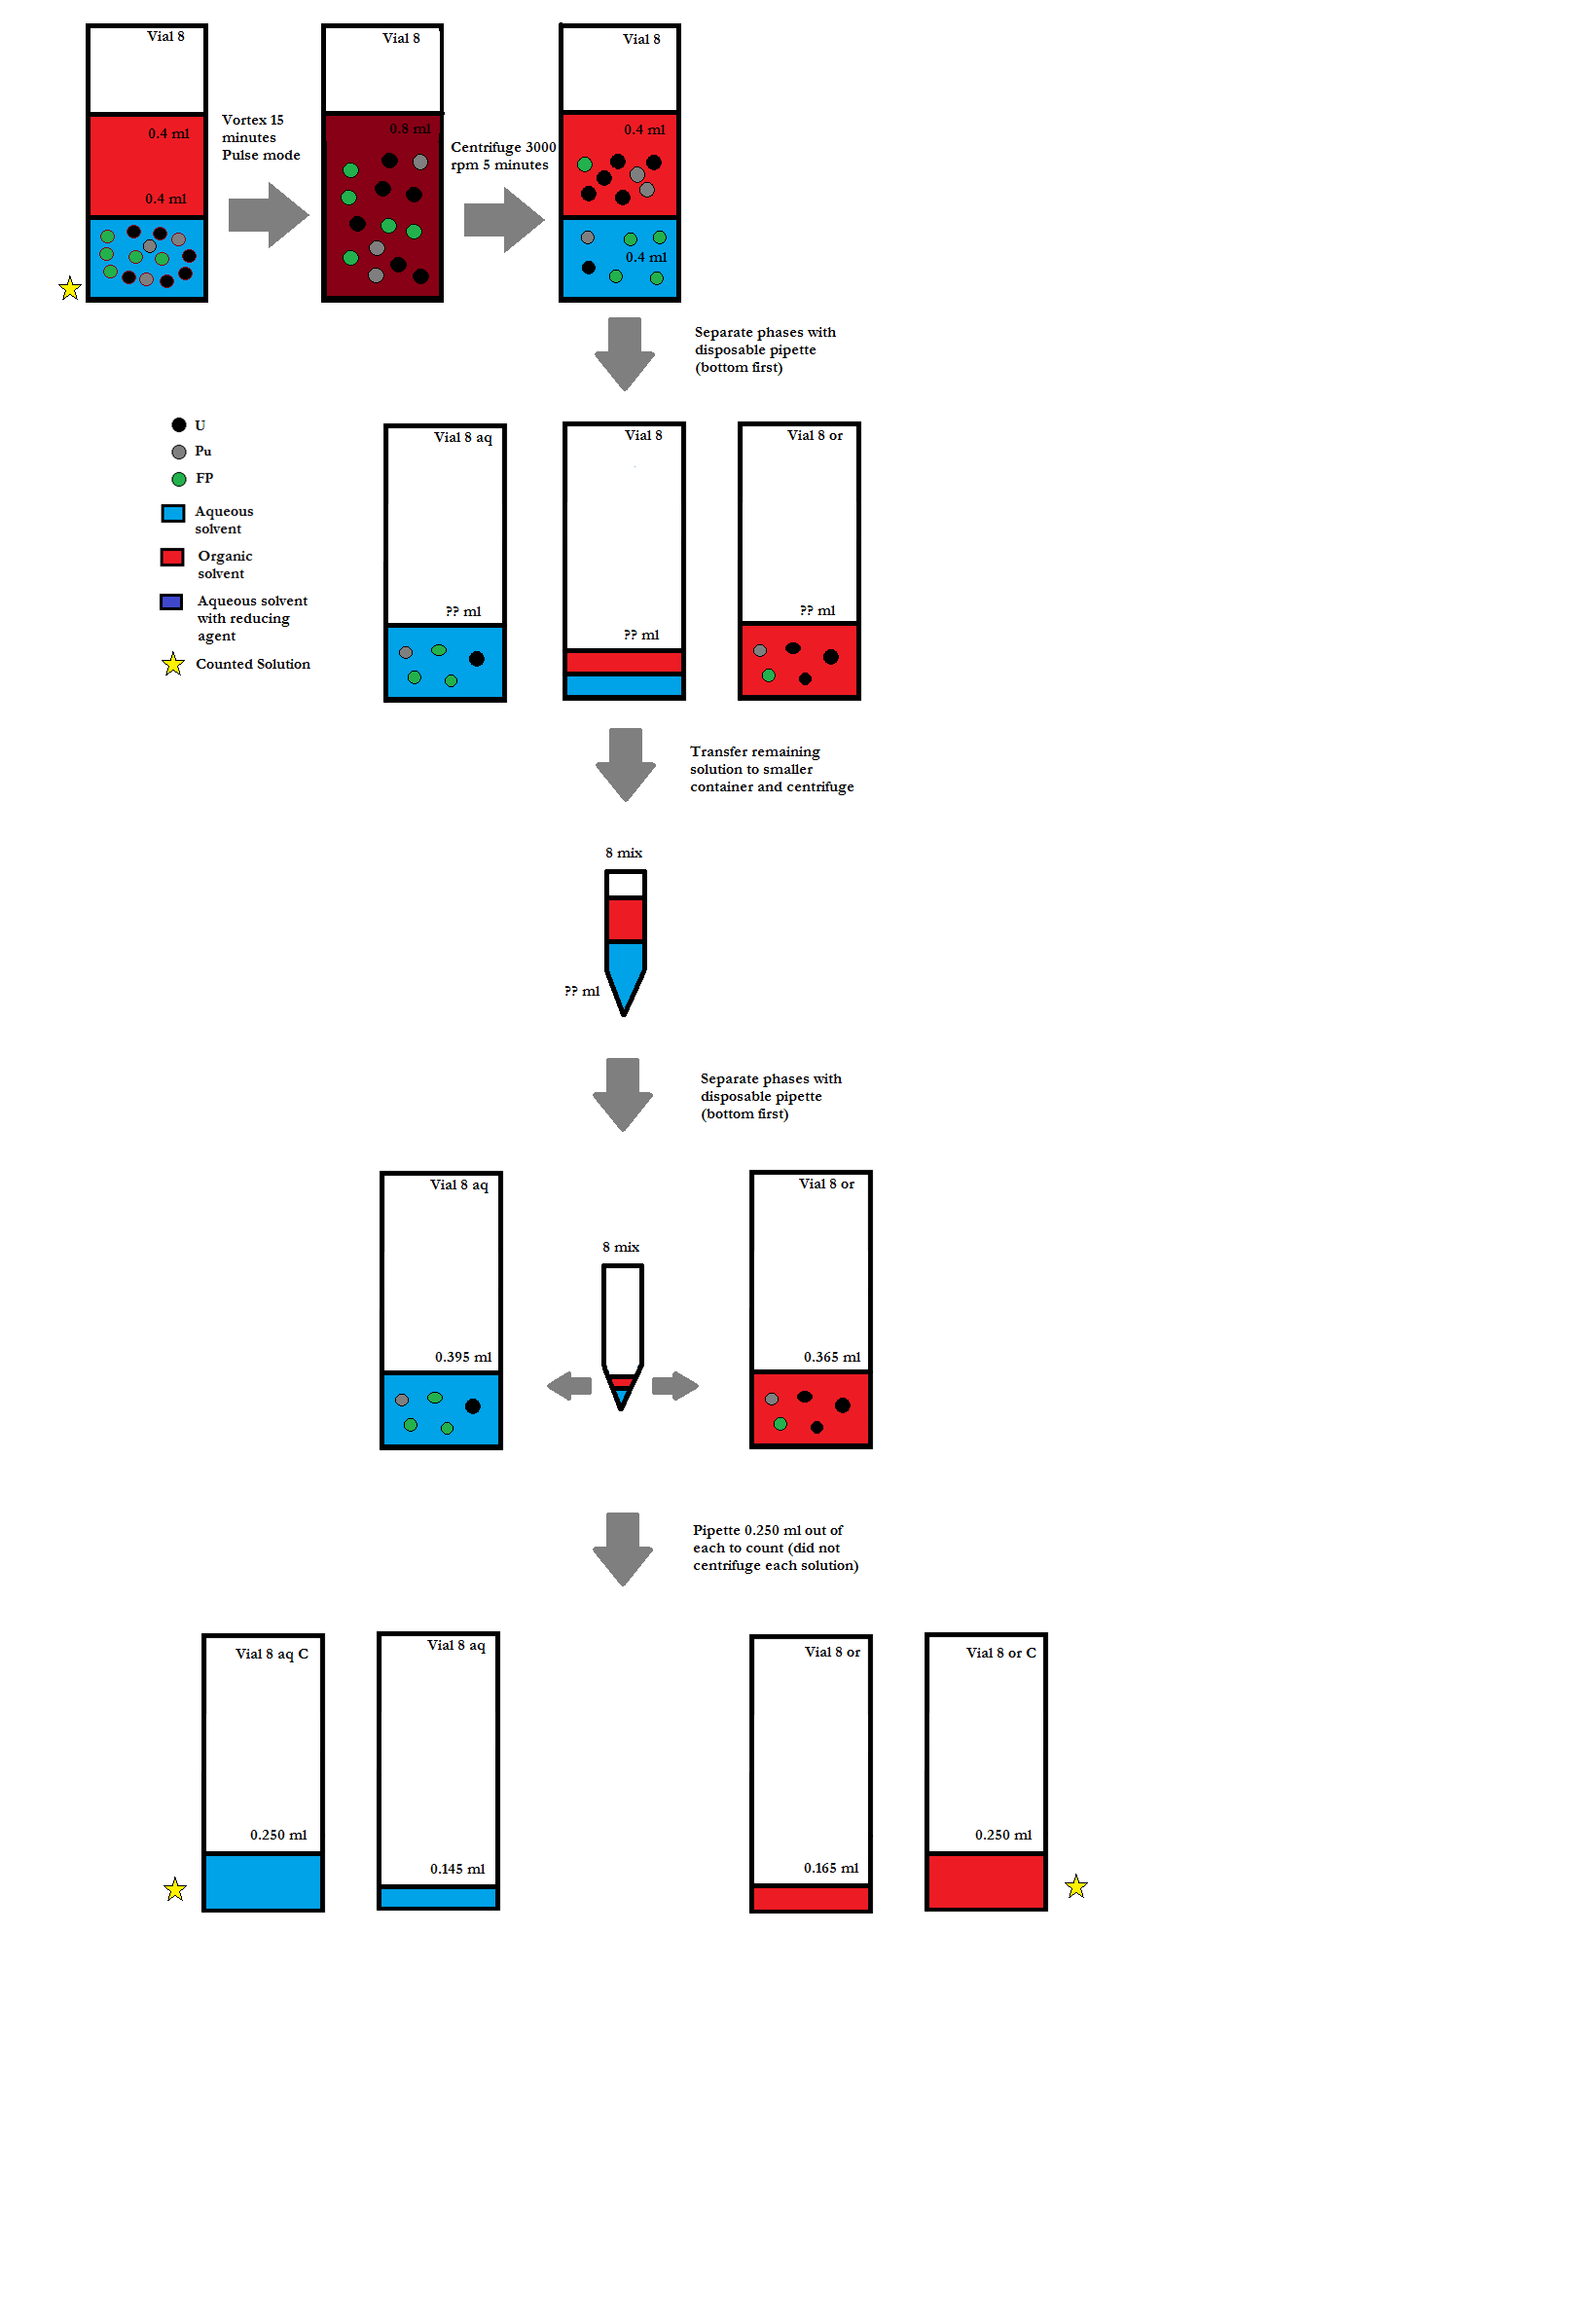
\includegraphics[width=0.8\linewidth]
                  {Figures/Cycle_x3_round_2}
\end{center}
\caption{Extraction three times round 2 experimental setup}
\label{fig:example2}
\end{figure}


%------------------------------------------------------------------------
%	LAB BOOK da
%-----------------------------------------------------------------------

\labday{Wednesday, 9 November 2016}


\experiment{Cycle_X3_round_2}
\begin{todolist}
\item[\done]{Finish count $\boxed{10\ or\ C}$}
  \begin{itemize}
  \item{Gave decent results for everything but \tss{137}Cs}
  \end{itemize}
\item[\done]{Start count $\boxed{10\ or\ C}$ on face of detector}
\item[\done]{Finish count $\boxed{10\ or\ C}$}
\item[\done]{Start count $\boxed{9\ or\ C}$ on face of detector}
\item[\done]{Analyze results from experiment, display in
  a single excel sheet}
  \begin{itemize}
  \item{Note GENIE corrects for dead time, but if you
    had to do it by hand, here is the equation for small
    corrections}
    \begin{equation*}
      CPS_f=\frac{CPS_i}{1-\frac{DT}{100}}
    \end{equation*}
  \end{itemize}
\end{todolist}

\experiment{ResearchMeeting}
\begin{itemize}
\item{Perfect \tss{137}Cs}
\item{Fix \tss{154}Eu}
\item{MARLAP, Stat teaching, look up MDA}
\item{Submit Degree plan, put a policy course on there}
\item{Subtracting BK is why I go negative sometimes,
  another reason for negative values in the D-value is
  because sometimes I take a difference}
\item{Covariance data is MT133}
\end{itemize}

%------------------------------------------------------------------------
%	LAB BOOK da
%-----------------------------------------------------------------------

\labday{Thursday, 10 November 2016}

\experiment{Cycle_X3_round_2}
\begin{todolist}
\item[\done]{Finish count $\boxed{9\ or\ C}$}
\item[\done]{Start count $\boxed{8\ or\ C}$ on face of detector ($\sim$ 4 pm)}
\item[\done]{Check if a geometric constant correction factor
  can be applied for the second geometry}
  \begin{itemize}
  \item{It can kind of be applied...\st{but not really}}
  \end{itemize}
\item[\done]{Looking at CPS for \tss{134}Cs between aqueous
  before extraction, and after (need to include volumes in
  calculation because each solution had different volumes)}
  \begin{itemize}
  \item{Did calculation for MDA, visually showed why
    we cant use the information...unless we count for a longer time}
  \end{itemize}
\end{todolist}

\experiment{School}

\begin{todolist}
\item{Alpha analysis}
\item{Respond to McClarren email - did this weekend}
\item{Review McClarrens notes email - did this weekend}
\item{Learn how to use ORIGEN - did this weekend}
\end{todolist}


%------------------------------------------------------------------------
%	LAB BOOK da
%-----------------------------------------------------------------------

\labday{Friday, 11 November 2016}

\experiment{Cycle_X3_round_2}
\begin{todolist}
\item[\done]{Finish count $\boxed{8\ or\ C}$}
\item[\done]{Start Efficiency count on face of detector}
\end{todolist}

\experiment{School}
\begin{todolist}
\item{Find variances}
\item[\done]{Learn how to use ORIGEN, and run it}
\item[\done]{Learn how to change the things in ORIGEN}
\item{Come up with chaos polynomial plan}
\item[\done]{Do a write up for McClarren...so it looks like
  I am doing work for his class}
\end{todolist}


%------------------------------------------------------------------------
%	LAB BOOK da
%-----------------------------------------------------------------------

\labday{Monday, 14 November 2016}

\experiment{Cycle_X3_round_2}

\begin{todolist}
\item[\done]{Finish Efficiency count on face of detector}
\item[\done]{Analyze results...something is very fishy}
  \begin{itemize}
  \item{The \tss{137}Cs results look very small 10\tss{-5}.
    Which we were hoping they would be around 0.01}
  \item{The other results had higher D-values across the board
    maybe due to geometric differences, maybe not}
  \end{itemize}
\item[\done]{Counted $\boxed{8\ aq\ C}$, $\boxed{9\ aq\ C}$,
  and $\boxed{10\ aq\ C}$ on the face of the detector (only needed
  to count each like 10 minutes or so (40\% dead time)}
  \begin{itemize}
  \item{To check and see if geometry is the issue (although these
    high dead times would probably give incorrect results - as
    Dr. Burns pointed out)}
  \end{itemize}
\item[\done]{Analyzed results from above counts, they increased
  the D-values to something more reasonable (similiar to the first
  experiment), but \tss{137}Cs is still acting like a punk
  ($\sim$ 10\tss{-5})}
  \begin{itemize}
  \item{Also noticed that Series 9 is a little funky...its always
    higher in D calculations by a large portion (except for Cs,
    where its lower)}
  \item{Frustrating!}
  \item{Dr. Kitcher brought up the issue that could be correcting to
    the wrong value (in series 6) - should find literature values}
  \item{Dr. Burns brought up that the fact that I didn't centrifuge
    the samples during the last step could be the issue}
  \item{Web of Knowledge, Web of Science, Periodic Table.com}
  \end{itemize}
\item[\done]{Recreate organic samples of $\boxed{8\ or\ C}$,
  $\boxed{9\ or\ C}$, and $\boxed{10\ or\ C}$.
  and count $\boxed{10\ or\ C}$ overnight}
  \begin{itemize}
  \item{Transfered above vials into glovebox - after parafilm wrapping}
  \item{Took all solution out of above vials, and put into original
    containers (labeled the same without the C - $\boxed{8\ or}$ as
    opposed to $\boxed{8\ or\ C}$)}
  \item{Centrifuged both C and non-C containers for 5 minutes on
    highest setting (33)}
  \item{Repipetted out 250 $\mu$l out of non-C containers into C
    containers}
  \item{Put C containers into 15 ml centrifuge tube}
  \item{Transfer out of glovebox and clean}
  \end{itemize}
\item[\done]{Dr. Burns found a reference with some useful data,
  \href{http://www.tandfonline.com/doi/abs/10.1080/07366298508918529}
       {Link}, table from reference below}
\end{todolist}
Quick calculation for molarity of uranium in samples
\begin{align*}
  \frac{0.0129\ \text{g DUO\tsbs{2}}\cdot 0.88 \cdot
  \frac{1}{238}}{0.005\
    \text{Liters}}=&0.009539M\\
  &0.009539\ \text{M}\cdot \frac{0.5\ ml}{2.5\ ml}\\
  =&0.001908\ \text{M U}
\end{align*}
Quick calculation for saturation of uranyl nitrate in water
at 20 \tss{o}C.
\begin{align*}
  \frac{122\ \text{g}}{\text{g}}=\frac{122\ \text{g}}{\text{g}}
    \cdot \frac{1000\ ml}{L}\cdot\frac{mol}{394.04\ g}\approx
    3.09 \text{M}
\end{align*}
\begin{table}[H]
\begin{center}
  \caption{Values from Paper, 1.4 M U (much higher than ours
    2 mM),
 and 3 M HNO\tsbs{3} (ours is at 4 M)}
\begin{tabular}{l l}
\toprule
Element & D-Value\\ 
Ru & $\boxed{0.04}$\\
Rh & 0.01\\
Pd & 0.09\\
Nd & 0.04\\
Ce & $\boxed{0.02}$\\
Sr & 0.00\\
Sm & 0.07\\
Cs & $\boxed{0.01}$\\
\bottomrule
\end{tabular}
\end{center}
\end{table}
The below figure shows that as the concentration
HNO\tsbs{3} increases from 3 to 4, we shouldn't expect
a huge difference between reference and our values.
Literature values should have some difference between 0\%
uranium saturation to 45\% saturation (reference)

\begin{figure}[H] % Example of including images
\begin{center}
  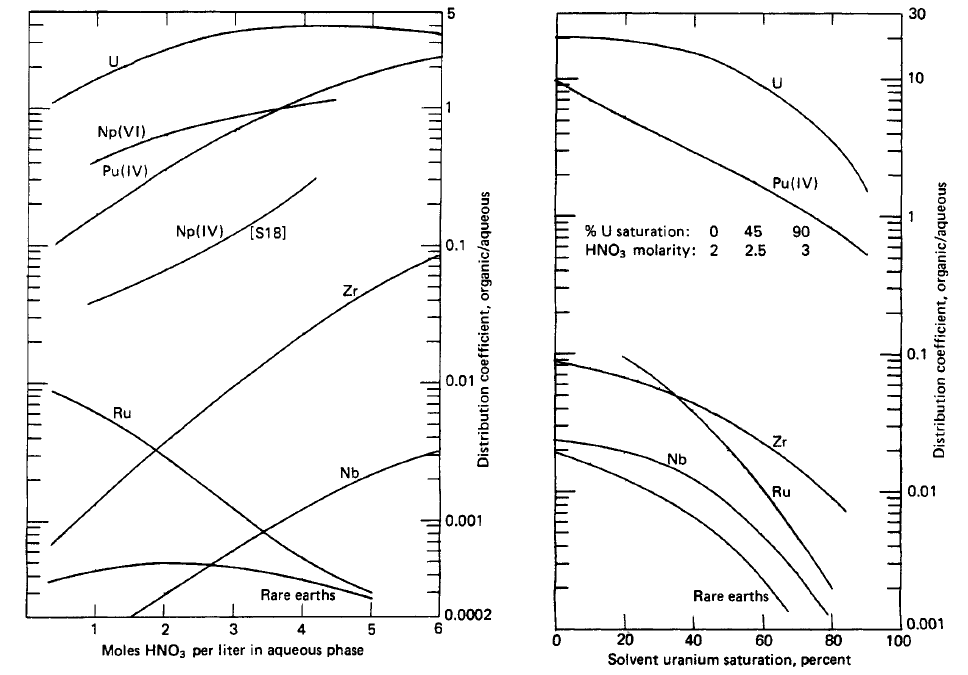
\includegraphics[width=0.8\linewidth]
                  {Figures/D_Values_Variations}
\end{center}
\caption{D value plots from Reactor handbook}
\label{fig:D_V_handbook}
\end{figure}






\begin{itemize}
\item{Ru, and Ce match from our experimental results from the first
  experiment,
  and Cs is around 0.01...which is what we are looking for,
  Sr there is no number (except that its small, which is in line
  with our first experiments). I also want to point out, no error bars,
  Dr. Folden would be not be happy, these numbers don't mean anything}
\end{itemize}
\begin{todolist}
\item[\done]{Looking at geometric differences between calibration
  source at 0 cm and 26 cm. and also between $\boxed{10\ or}$ at
  0 cm and 26 cm.}
  \begin{itemize}
  \item{Noticed there is a trend, might be able to use}
  \item{Also noticed that I counted my \tss{152}Eu source at
    26 cm for a short time (1.9 live time hours)...
    will start count for that in
    the morning and count while doing the experiment,
    maybe that will fix some problems. The reason for this
    short count time, is I feel lots of pressure to finish}
  \end{itemize}
\end{todolist}


%------------------------------------------------------------------------
%	LAB BOOK da
%-----------------------------------------------------------------------

\labday{Tuesday, 15 November 2016}

\experiment{Cycle_X3_round_2}

\begin{todolist}
\item[\done]{Stop count of $\boxed{10\ or\ C}$ around 5:50 am}
\item[\done]{Start efficency count at 26 cm around 5:50 am}
\item[\done]{Analyze results from $\boxed{10\ or\ C}$}
  \begin{itemize}
  \item{Counts for Ce, look better, Eu look better,
    Ru look worse, Cs look better (but still one order of magnitude
    off}
  \item{Looking into the count rates, some peaks change by
    alot between the first and second count of $\boxed{10\ or\ C}$
    and the second...WHY!?}
  \item{Maybe because some aqueous was in the original sample
    $\boxed{10\ or}$, and because it had some time to dissolve into
    the solution, the activities for the lower D materials increased}
  \end{itemize}
\end{todolist}

\experiment{Cycle_X3_round_2_alpha}
\begin{todolist}
\item[\done]{Label vials: $\boxed{8,9,10\ Dilution}$,
  $\boxed{8\ aq\ Dilution}$,
  $\boxed{9\ aq\ Dilution}$,
  $\boxed{10\ aq\ Dilution}$,
  $\boxed{8\ or\ Dilution}$,
  $\boxed{9\ or\ Dilution}$,
  $\boxed{10\ or\ Dilution}$.
  Label Chips: $\boxed{8\ Chip}$, $\boxed{9\ Chip}$,
  $\boxed{10\ Chip}$,
  $\boxed{8\ aq\ Chip}$, $\boxed{9\ aq\ Chip}$,
  $\boxed{10\ aq\ Chip}$,
  $\boxed{8\ or\ Chip}$, $\boxed{8\ or\ Chip}$,
  $\boxed{10\ or\ Chip}$}
  \begin{todolist}
  \item[\done]{Also transfer 3 red and 4 blue push caps for smaller vials}
  \end{todolist}
\item[\done]{Transfer all above vials and chips into glovebox}
\end{todolist}

\experiment{Cycle_X3_round_2}

\begin{todolist}
\item[\done]{Finish Eff count}
  \begin{itemize}
  \item{Rework calculations with new eff...didn't help much}
  \end{itemize}
\item[\done]{Start $\boxed{9\ or}$ count}
\item[\done]{Spend all night making spreadsheet to calculate
  how much volume would be optimal for contamination in
  each series}
  \begin{itemize}
  \item{It made things kind of work better, but not a whole lot better}
  \item{Reason why I haven't averaged numbers yet...was taking a
    26 counting efficency, counted most of the day}
  \item{Also determined geometric differences between calculating
    activity at 0 cm as opposed to 26 cm - there wasn't much
    of a difference}
  \item{Also, need to complete recounts for $\boxed{8\ or\ C}$ and
    $\boxed{9\ or\ C}$}
  \end{itemize}
\end{todolist}



%------------------------------------------------------------------------
%	LAB BOOK da
%-----------------------------------------------------------------------

\labday{Wednesday, 16 November 2016}

\begin{todolist}
\item[\done]{Transfer in the glovebox a blue 2.5 ml vial
  (also hold smaller conical
  vials) holder - sorry Mary, it makes things much easier to
  have something to hold your vials}
\item[\done]{Transfer smaller pipette tips into glovebox}
\item[\done]{take out the trash in the glovebox}
\end{todolist}

\experiment{Cycle_X3_round_2}

\begin{todolist}
\item[\done]{Finish count $\boxed{9\ or}$}
\item[\done]{Begin count $\boxed{8\ or}$ (9:44 am)}
\end{todolist}


\experiment{Cycle_X3_round_2_alpha}

\begin{todolist}
  
\item[\done]{Make alpha sample of stock, make 3 (
      Pipette Errors - assume 20 $\mu$l error 1\%,
      10 $\mu$l error 1.2\%, 390 $\mu$l error 2\%, 890 $\mu$l error 1\%)}
\end{todolist}
\begin{center}
  10+/-0.12 $\mu$l of $\boxed{Stock\ Add}$ (4 M HNO\tsbs{3})
  [smaller pipette]\\
+\\
990+/-9.9 $\mu$l of DI water (leftover in glovebox)\\
=\\
1+/-9.9 ml of $\sim$ 0 M HNO\tsbs{3} $\boxed{8,9,10\ Dilution}$
\end{center}
\vspace{0.3cm}
\begin{center}
  20+/-0.2 $\mu$l of $\boxed{8,9,10\ aq\ Dilution}$ dropped onto
  $\boxed{8\ Chip}$
\end{center}
\begin{center}
  20+/-0.2 $\mu$l of $\boxed{8,9,10\ aq\ Dilution}$ dropped onto
  $\boxed{9\ Chip}$
\end{center}
\begin{center}
  20+/-0.2 $\mu$l of $\boxed{8,9,10\ aq\ Dilution}$ dropped onto
  $\boxed{10\ Chip}$
\end{center}
\begin{todolist}

  
\item[\done]{Make alpha sample of each aqueous}
\begin{todolist}
\item[\done]{- $\boxed{8\ aq}$}
\end{todolist}
\begin{center}
10+/-0.12 $\mu$l of $\boxed{8\ aq}$ (4 M HNO\tsbs{3}) [smaller pipette]\\
+\\
390+/-7.8 $\mu$l of DI water (leftover in glovebox)\\
=\\
0.4+/-0.0078 ml of $\sim$ 0 M HNO\tsbs{3} $\boxed{8\ aq\ Dilution}$
\end{center}
\begin{itemize}
\item{$\boxed{8\ aq}$ transfer contaminated gloves (had the blue
  push cap) and the vial accidentally fell}
\end{itemize}
\vspace{0.3cm}
\begin{center}
  20+/-0.2 $\mu$l of $\boxed{8\ aq\ Dilution}$ dropped onto
  $\boxed{8\ aq\ Chip}$
\end{center}
\begin{todolist}
\item[\done]{- $\boxed{9\ aq}$}
  \begin{itemize}
  \item{$\boxed{9\ aq}$ and $\boxed{10\ aq}$ centrifuged, so
    no contamination on glovebox gloves like above}
  \end{itemize}
\end{todolist}
\begin{center}
10+/-0.12 $\mu$l of $\boxed{9\ aq}$ (4 M HNO\tsbs{3}) [smaller pipette]\\
+\\
390+/-7.8 $\mu$l of DI water (leftover in glovebox)\\
=\\
0.4+/-0.0078 ml of $\sim$ 0 M HNO\tsbs{3} $\boxed{9\ aq\ Dilution}$
\end{center}
\vspace{0.3cm}
\begin{center}
  20+/-0.2 $\mu$l of $\boxed{9\ aq\ Dilution}$ dropped onto
  $\boxed{9\ aq\ Chip}$
\end{center}
\begin{todolist}
\item[\done]{- $\boxed{10\ aq}$}
\end{todolist}
\begin{center}
10+/-0.12 $\mu$l of $\boxed{10\ aq}$ (4 M HNO\tsbs{3}) [smaller pipette]\\
+\\
390+/-7.8 $\mu$l of DI water (leftover in glovebox)\\
=\\
0.4+/-0.0078 ml of $\sim$ 0 M HNO\tsbs{3} $\boxed{10\ aq\ Dilution}$
\end{center}
\vspace{0.3cm}
\begin{center}
  20+/-0.2 $\mu$l of $\boxed{10\ aq\ Dilution}$ dropped onto
  $\boxed{10\ aq\ Chip}$
\end{center}


\item[\done]{Make alpha sample of each organic phase}
\begin{todolist}
\item[\done]{- $\boxed{8\ or}$}
\end{todolist}
\begin{center}
10+/-0.12 $\mu$l of $\boxed{8\ or}$ (30\% TBP) [smaller pipette]\\
+\\
890+/-8.9 $\mu$l of 30\% TBP (leftover in glovebox)\\
=\\
0.9+/-0.0089 ml of 30\% TBP $\boxed{8\ or\ Dilution}$
\end{center}
\vspace{0.3cm}
\begin{center}
  20+/-0.2 $\mu$l of $\boxed{8\ or\ Dilution}$ dropped onto
  $\boxed{8\ or\ Chip}$
\end{center}
\begin{itemize}
\item{\textbf{Spilled some organic on inner ring??
    of $\boxed{8\ or\ Chip}$, question because hard to see in
    glovebox}}
\end{itemize}
\begin{todolist}
\item[\done]{- $\boxed{9\ or}$}
\end{todolist}
\begin{center}
10+/-0.12 $\mu$l of $\boxed{9\ or}$ (30\% TBP) [smaller pipette]\\
+\\
890+/-8.9 $\mu$l of 30\% TBP (leftover in glovebox)\\
=\\
0.9+/-0.0089 ml of 30\% TBP $\boxed{9\ or\ Dilution}$
\end{center}
\vspace{0.3cm}
\begin{center}
  \textbf{10}+/-0.12 $\mu$l of $\boxed{9\ or\ Dilution}$ dropped onto
  $\boxed{9\ or\ Chip}$
\end{center}
\begin{itemize}
\item{\textbf{Changed volume on chip because $\boxed{8\ or\ Chip}$
    potentially spilled over the inner ring}}
\end{itemize}
\begin{todolist}
\item[\done]{- $\boxed{10\ or}$}
\end{todolist}
\begin{center}
10+/-0.12 $\mu$l of $\boxed{10\ or}$ (30\% TBP) [smaller pipette]\\
+\\
890+/-8.9 $\mu$l of 30\% TBP (leftover in glovebox)\\
=\\
0.9+/-0.0089 ml of 30\% TBP $\boxed{10\ or\ Dilution}$
\end{center}
\vspace{0.3cm}
\begin{center}
  \textbf{10}+/-0.12 $\mu$l of $\boxed{10\ or\ Dilution}$ dropped onto
  $\boxed{10\ or\ Chip}$
\end{center}
\begin{itemize}
\item{\textbf{Changed volume on chip because $\boxed{8\ or\ Chip}$
    potentially spilled over the inner ring}}
\end{itemize}
\item[\done]{\textbf{Note: Centrifuged all dilution vials before making
    alpha samples, which means that first all dilutions were made,
    then all alpha samples were made}}
\item[\done]{The above 7 alpha samples take up space in the
  glovebox, and I didn't want to disturb the samples (moving them
  screws them up) so I let them dry overnight}
\end{todolist}


\experiment{Process_X3}
\begin{todolist}
\item[\done]{Combine all aqueous phases together (done with disposable
pipetets)}
  \begin{todolist}
  \item[\done]{$\boxed{8\ aq\ C}+\boxed{8\ mix}\ \rightarrow\ \boxed{8\ aq}$
    (take all of first and add to second)}
  \item[\done]{$\boxed{9\ aq\ C}+\boxed{9\ mix}\ \rightarrow\ \boxed{9\ aq}$}
  \item[\done]{$\boxed{10\ aq\ C}+\boxed{10\ mix}\ \rightarrow\ \boxed{10\ aq}$}
  \end{todolist}
\end{todolist}

\experiment{ResearchMeeting}

\begin{itemize}
\item{Just present D-Values at research meeting}
\item{Things didn't add up so well}
\item{Dr. Chirayath didn't like my \tss{137}Cs values,
  looked at the first experiment, the one where
  I messed up, and liked the 110 value, now I
  am getting 10\tss{-5}...why?}
\item{Dr. Burns suggested to increase the volume
  of the extraction phase (organic) to pin
  down the \tss{137}Cs values}
\item{Dr. Folden also said that we should average
  the percent extraction values, not the D-values,
  because D values vary widly at the ends (shown in
  next figure)}
\end{itemize}
\begin{equation*}
  \text{Fraction Extracted}=\frac{\text{Mass Organic}}{\text{Mass Initial}}
\end{equation*}
\begin{itemize}
\item{Dr. Chirayath said to continue process}
\item{Jeremy had interesting results, the flux spectra
  turned from kind of fast to thermal, Gd burned out}
\item{Robert Zedric also noted that a higher dead time
  could be used, and that our detector is between
  a Nonparalyzable and paralyzable model, and that
  we could try to work through the math on that,
  Knoll page 122}
\end{itemize}

\begin{figure}[H] % Example of including images
\begin{center}
  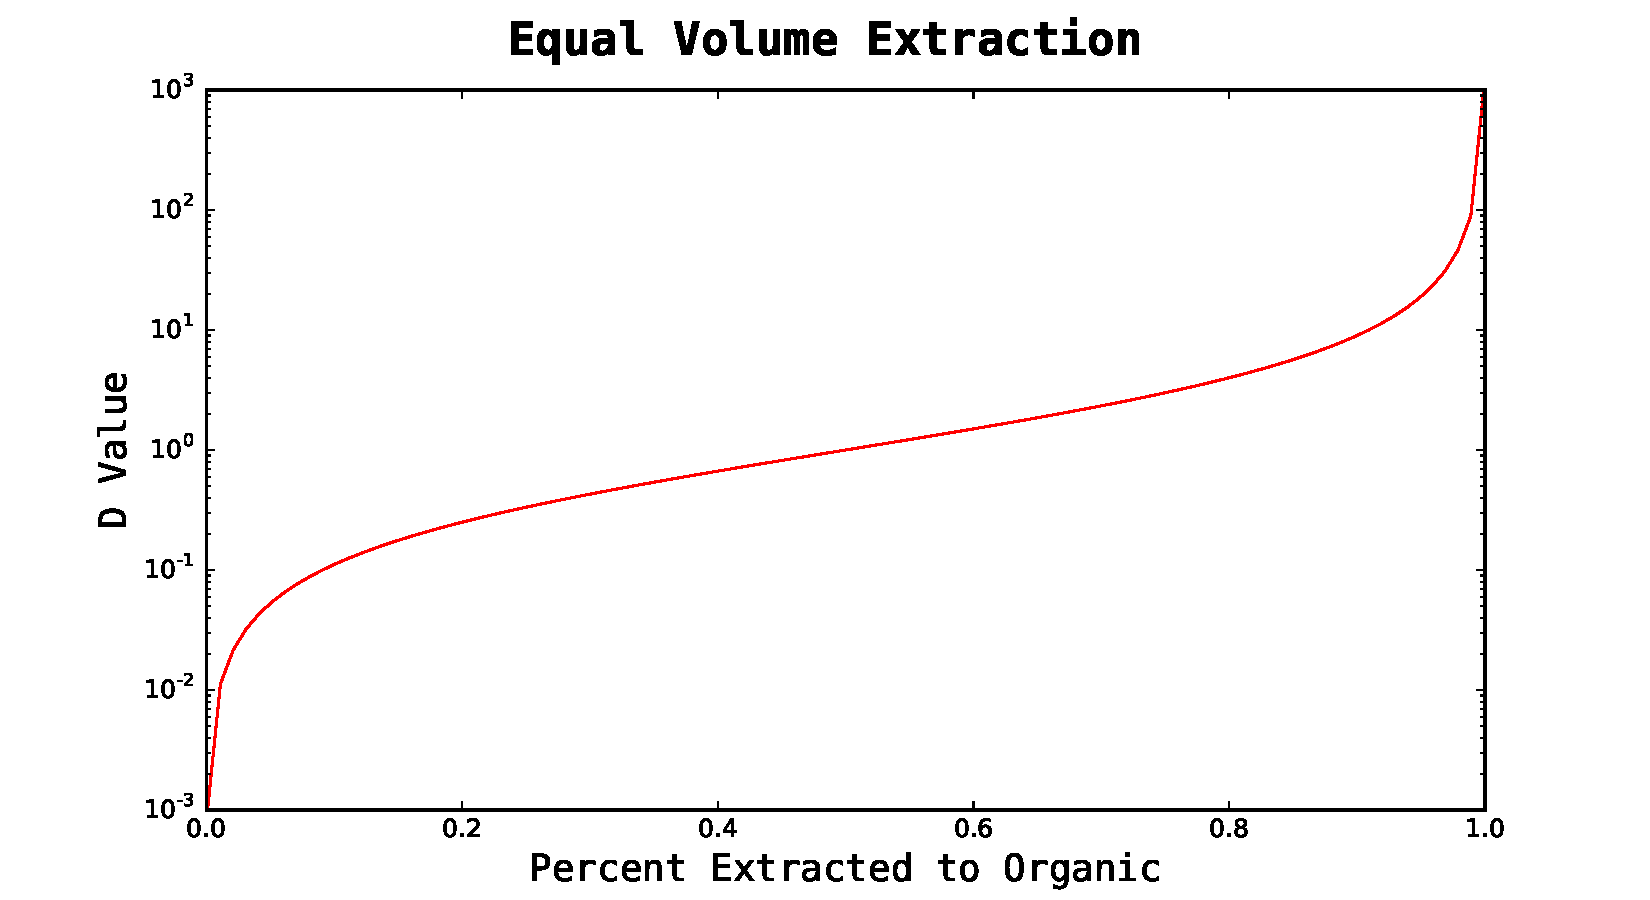
\includegraphics[width=0.8\linewidth]
                  {Figures/Percent_Extraction_vs_D_Value_log}
\end{center}
\caption{Percent extraction versus D value on log scale}
\label{fig:P_Ext}
\end{figure}


%------------------------------------------------------------------------
%	LAB BOOK day
%-----------------------------------------------------------------------

\labday{Thursday, 17 November 2016}


\experiment{Cycle_X3_round_2_alpha}
Note all alpha counts were done on the 9mm height setting
on the pips detector.
\begin{todolist}
\item[\done]{Start Count $\boxed{10\ or\ Chip}$ (10:52 am)}
\item[\done]{End Count $\boxed{10\ or\ Chip}$ Run time 7.54 hrs}
\item[\done]{Start count $\boxed{10\ aq\ Chip}$ (6:29 pm)}
\end{todolist}


\experiment{56_run}

In order to capture the D-value for \tss{137}Cs,
an experiment was proposed. Our problem with measuring
\tss{137}Cs is that its D-value and activity are so low
that we aren't getting good statistics for its answer,
and the answer we are getting is not the answer we want,
we are getting something around 10\tss{-5}, and the answer
is more probably around 0.01.
\vspace{0.3cm}

It was proposed to take an old series (series 5 or 6), and
perform an extraction with a larger volume of organic,
so that more \tss{137}Cs could be extracted, and therefore
better statistics on all the calculations. Some notes
are copied down from hand calculations for the experiment.
\begin{itemize}
\item{$\boxed{5\ aq}$ has 461 $\mu$l, 4.47 $\mu$Ci, $\sim$ 3.6\% dead time}
\item{$\boxed{6\ aq}$ has 469 $\mu$l, 4.40 $\mu$Ci, $\sim$ 3.6\% dead time,
  this vial is also a little milky, meaning there is a small amount
  of organic in there}
\item{Both above vials should were in fumehood}
\item{Some evaporation happened in $\boxed{Stock}$,
  I know this because the activity density changed from
  $\boxed{Stock}$ and $\boxed{Stock\ add}$.}
\item{If we take 800 $\mu$l total (after mixing $\boxed{5\ aq}$
  and $\boxed{6\ aq}$), then we could expect $\sim$ 8.87 $\mu$l
  (about 200 cps),
  of \tss{137}Cs with $\sim$ 6\% dead time}
\item{If we want 3 cps in the final organic
  (about an hour of count time) and if I assume the D-value
  is 0.01 (which Dr. Chirayath insists), (3/200 $\sim$ 1.5\%
  of the counts)}
\end{itemize}
\begin{align*}
  \%=&\frac{1}{1+\frac{V_a}{V_o}\frac{1}{D}}\\
  =&\frac{1}{1+\frac{1}{2}\frac{1}{0.01}}=0.019
\end{align*}
This means if we double the volume of the organic, then
we should get a decent count rate so as to count \tss{137}Cs
and get good statistics with an hour count. This is IF
the D-value is 0.01, as Dr. Chirayath insists.
\begin{itemize}
\item{Dr. Burns came by and said, instead of 2x the organic volume,
  should do 10x, to make sure we get all the counts!}
\item{Okay! Sounds good! We will for sure get the right answer
  now! We also rederived the D-value equation}
\end{itemize}
With conservation of mass, and using values from the two phases,
\begin{align*}
  \text{\% Extracted}=&\frac{[\frac{CPS}{V_{m}}]_o\cdot V_{co}}
       {[\frac{CPS}{V_{m}}]_o\cdot V_{co}+
         [\frac{CPS}{V_{m}}]_a\cdot V_{ca}}\\~\\
       \frac{1}{\text{\% Extracted}}
       =&\frac{[\frac{CPS}{V_{m}}]_o\cdot V_{co}+
         [\frac{CPS}{V_{m}}]_a\cdot V_{ca}}
       {[\frac{CPS}{V_{m}}]_o\cdot V_{co}}\\~\\
       =&1+\frac{[\frac{CPS}{V_m}]_a\cdot V_{ca}}
       {[\frac{CPS}{V_m}]_o\cdot V_{co}}\\~\\
       =&1+\frac{1}{D}\cdot\frac{V_{ca}}{V_{co}}\\~\\
       \frac{1}{\frac{V_{co}}{V_{ca}}\left(\frac{1}{\text{\% Extracted}}-1
       \right)}
       =&D
\end{align*}
Where $V_m$ is the measured volume for the count, $V_{co}$ is
the volume of the organic contact and $V_{ao}$ is the volume
of the aqueous contact. 

\begin{todolist}
\item[\done]{Combine $\boxed{5\ aq}$ and $\boxed{6\ aq}$
  into $\boxed{5\ aq}$}
\item[\done]{Take 800 $\mu$l out of $\boxed{5\ aq}$ and transfer
  into a 15 ml vial labeded $\boxed{56}$ (for some reason
  it was really difficult to get a precise volume - had to do
  many times)}
\item[\done]{Start count $\boxed{56}$ at 26 cm}
\end{todolist}

\experiment{Cycle_X3_round_2}

\begin{todolist}
\item[\done]{Finish count $\boxed{8\ or}$ ($\sim$ 9:45 am)
  about this time another count was started - vial 56,
  described above}
\item[\done]{Analyzed last two organics, put into excel
  sheet}
  \begin{itemize}
  \item{All samples of organic, after mixing organic parts together,
    redrawing 250 $\mu$l and recounting, increased in activity.
    This could support the conclusion that some aqueous passed
    to the main organic, and when the 250 $\mu$l was first drawn,
    was on the bottom of the vial. When the 250 $\mu$l was second
    drawn, it had time to dissolve into the TBP, because
    HNO\tsbs{3} is slightly soluble in TBP (
    Nuclear Chemical Engeineering pg 160)}
  \end{itemize}
\end{todolist}

\experiment{Process_X3}
\begin{todolist}
\item[\done]{Measure volumes of all aqueous phases, $\boxed{8\ aq}$
     $\boxed{9\ aq}$, $\boxed{10\ aq}$}
\begin{table}[H]
  \begin{center}
    \caption{Volumes for combined aqueous phases}
    \begin{tabular}{l l l}
      \toprule
      Series & Aqueous (8,9, or 10)\\ 
      8 & 397 +/- 7.94\\
      9 & \st{386} 389 +/- 7.78 (after centrifuge)\\
      10 & 395 +/- 7.9\\
      \bottomrule
    \end{tabular}
  \end{center}
\end{table}  
\end{todolist}

Second Contact...

\begin{todolist}
\item[\done]{Label vials,
  $\boxed{8\ aqII}$,  $\boxed{8\ aqII\ C}$,  $\boxed{8\ orII}$,
  $\boxed{8\ orII\ C}$
  $\boxed{9\ aqII}$,  $\boxed{9\ aqII\ C}$,  $\boxed{9\ orII}$,
  $\boxed{9\ orII\ C}$
  $\boxed{10\ aqII}$, $\boxed{10\ aqII\ C}$, $\boxed{10\ orII}$,
  $\boxed{10\ orII\ C}$ (smaller 2.5 ml tubes)}
  \begin{itemize}
  \item{Will reuse $\boxed{8\ mix}$, $\boxed{9\ mix}$,
    $\boxed{10\ mix}$ (smaller 1 ml tubes from John Burns,
    have conical bottoms, makes more minute separations easier)}
  \end{itemize}
  
\item[\done]{Transfer:
  $\boxed{8\ aqII}$,  $\boxed{8\ aqII\ C}$,  $\boxed{8\ orII}$,
  $\boxed{8\ orII\ C}$
  $\boxed{9\ aqII}$,  $\boxed{9\ aqII\ C}$,  $\boxed{9\ orII}$,
  $\boxed{9\ orII\ C}$
  $\boxed{10\ aqII}$, $\boxed{10\ aqII\ C}$, $\boxed{10\ orII}$,
  $\boxed{10\ orII\ C}$.
  (3 clear push caps, and 6 blue push caps
  6 red push caps). Also with 6 15 ml centrifuge tubes}
\item[\done]{Add 397 $\mu$l of $\boxed{TBP}$ to $\boxed{8\ aq}$}
\item[\done]{Add 389 $\mu$l of $\boxed{TBP}$ to $\boxed{9\ aq}$}
\item[\done]{Add 396 $\mu$l of $\boxed{TBP}$ to $\boxed{10\ aq}$}
\item[\done]{Vortex mix $\boxed{8\ aq}$ for 15 minutes on pulse mode}
\item[\done]{Centrifuge $\boxed{8\ aq}$ with $\boxed{Buddy}$ at 3,300
  rpm for 10 minutes}
  \begin{itemize}
  \item{Decieded after this to wait, and centrifuge them all together}
  \end{itemize}
\item[\done]{Vortex mix $\boxed{9\ aq}$ for 15 minutes on pulse mode}
\item[\done]{Vortex mix $\boxed{10\ aq}$ for 15 minutes on pulse mode}
\item[\done]{Centrifuge $\boxed{8\ aq}$, $\boxed{9\ aq}$,
  and $\boxed{10\ aq}$
  with $\boxed{Buddy}$ on 3300 rpm, for 5 minutes}
\item{\st{During the vortex mixing and the centrifuge
  practice the transfer in the fumehood} Prayed instead}
\item[\done]{Pipette with disposable pipette the organic phase
  first, then the aqueous (for all three vials),
  as much as so that there is no mixing.
  Then transferred the boundary to a smaller vial, let sit.
  Prepare counting solutions of 250 $\mu$l of each of the solutions
  A picture will be provided for the whole process for $\boxed{8\ aq}$
  on the following page
  , below are specific notes about what
  occured during the experiment.}
  \begin{itemize}
  \item{$\boxed{8\ aq}$ was 248 $\mu$l pipetted to $\boxed{8\ aqII\ C}$
  instead of 250 $\mu$l?}
  \end{itemize}
\item{\st{Measure volumes of everything}}
\item[\done]{Transfer out $\boxed{8\ orII\ C}$, $\boxed{8\ aqII\ C}$,
  $\boxed{9\ orII\ C}$, $\boxed{9\ aqII\ C}$, $\boxed{10\ orII\ C}$,
  $\boxed{10\ aqII\ C}$, in 15 ml centrifuge tubes}
\item[\done]{Radiac wash the above tubes, and store in fumehood behind
  lead - wait to count}
\item[\done]{Clean stuff in glovebox}
\item[\done]{Start count $\boxed{9\ orII\ C}$ at 0 cm 4:06 pm}
\end{todolist}

\begin{figure}[H] % Example of including images
\begin{center}
  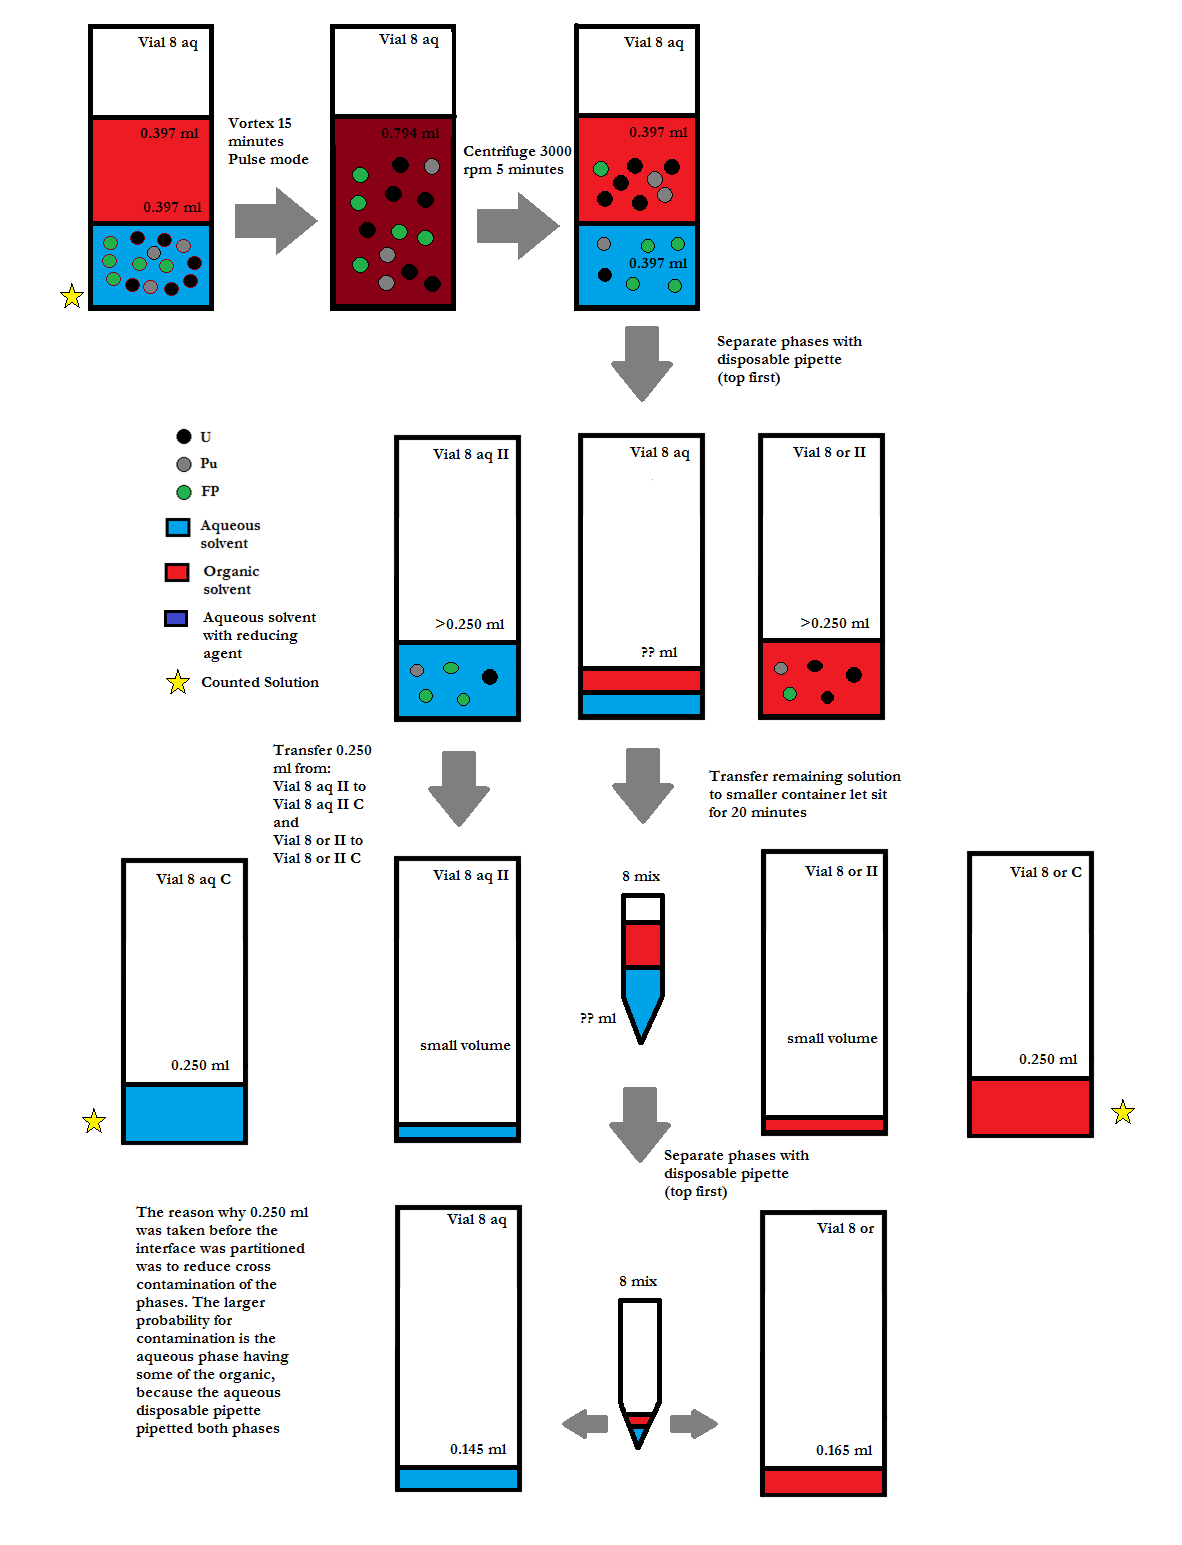
\includegraphics[width=0.8\linewidth]
                  {Figures/Cycle_x3_round_2_extraction_2}
\end{center}
\caption{Extraction three times round 2 extraction 2}
\label{fig:round2_extraction2}
\end{figure}



%------------------------------------------------------------------------
%	LAB BOOK day
%-----------------------------------------------------------------------

\labday{Friday, 18 November 2016}



\experiment{Cycle_X3_round_2_alpha}
Note all alpha counts were done on the 9mm height setting
on the pips detector.
\begin{todolist}
\item[\done]{End Count $\boxed{10\ aq\ Chip}$ Run time 14.4 hrs}
\item[\done]{Start Count $\boxed{9\ or\ Chip}$ (9:02 am)}
\item[\done]{End Count $\boxed{9\ or\ Chip}$ Run time 6.08 hrs}
\item[\done]{Start count $\boxed{9\ aq\ Chip}$ (3:11 pm)}
\end{todolist}



\experiment{Process_X3}

\begin{todolist}
\item[\done]{End count $\boxed{9\ orII\ C}$ RunTime 16.5 hr}
\item[\done]{Start count $\boxed{8\ orII\ C}$ at 0 cm 8:56 am
             end around 11:15 pm (count  $\boxed{56\ Big}$)}
\item[\done]{End count $\boxed{8\ orII\ C}$ (RunTime 2.254 hrs)}
\item[\done]{Start count $\boxed{10\ orII\ C}$ at 0 cm 1:04 pm}
\end{todolist}


\experiment{56_run}
Talked about volume changes with Kevin, using 50 ml tubes
for the whole experiment
\begin{todolist}
\item[\done]{Transfer $\boxed{56}$ into glovebox with labeled
  50 ml tubes $\boxed{56\ Big}$, $\boxed{56\ Big\ Aq}$,
  and $\boxed{56\ Big\ or}$}
\item[\done]{Take the 800 $\mu$l out of $\boxed{56}$, and
  transfer to $\boxed{56\ Big}$ (had to do middle step of
  transfering everything to $\boxed{5 \ aq}$)}
\item[\done]{Take $\boxed{56\ Big}$ out of glovebox}
\item[\done]{Start count $\boxed{56\ Big}$ (11:17 am) to
             around 1:04 (started count $\boxed{10\ orII\ C}$}
\end{todolist}
Just prior to stopping the above count, Dr. Burns suggested
keeping all 800 $\mu$l of the aqueous in $\boxed{56}$ instead
of $\boxed{56\ Big}$ and just but all organic into a 50 ml tube.
So now...
\begin{todolist}
\item[\done]{Transfer $\boxed{56\ Big}$ into glovebox (wrapped
  in a ziplock bag so that less evaporation)}
\item[\done]{Transfer 800 $\mu$l out of $\boxed{56\ Big}$ into
  $\boxed{56}$}
\item[\done]{Add 8.0 $\mu$l of TBP to $\boxed{56}$}
\item[\done]{Shake $\boxed{56}$ on vortex mixer for 15 minutes}
\item[\done]{Convert a 2.5 ml vial holder (a 15 ml tube) to a
  buddy, by adding 800 $\mu$l of DI water and 8.0 ml of TBP
  to it...scratch out label. $\boxed{56\ Buddy}$}
\item[\done]{Centrifuge $\boxed{56}$ with $\boxed{56\ Buddy}$
  for 15 minutes at 3,300 rpm}
\item[\done]{Carefully pipette with disposable pipette,
  as much of top phase of $\boxed{56}$ as possible to
  $\boxed{56\ Or}$ (50 ml tube)}
\item[\done]{Carefully pipette with new disposable pipette,
  the bottom phase of $\boxed{56}$ (aq) to $\boxed{56\ aq}$ (15 ml tube)}
\item[\done]{Clean up work area in glovebox}
\item[\done]{Transfer interface of $\boxed{56}$ to $\boxed{56\ mix}$,
  seal and let sit for the time being}
\item[\done]{Transfer out of glovebox
  $\boxed{56\ aq}$ and $\boxed{56\ or}$. Clean with radiac wipes}
\item[\done]{Count $\boxed{56\ or}$ (2:28 pm),
  expecting 20 cps (calculation below,
  where 0.01 is the expected D-value of \tss{137}Cs)}
\end{todolist}
\begin{align*}
  \frac{200\ \text{cps\tsbs{aq}}}{800\ \mu\text{l}}\cdot8,000\ \mu\text{l}
  \cdot0.01=20\ \text{cps\tsbs{or}}
\end{align*}
Sadly, first glance gives around 0.1 cps\tsbs{or}, I have failed again.
Sorry Dr. Chirayath. I am feeling fairly defeated, I just want to go home.


%------------------------------------------------------------------------
%	LAB BOOK day
%-----------------------------------------------------------------------

\labday{Sunday, 20 November 2016}

\experiment{Cycle_X3_round_2_alpha}
Note all alpha counts were done on the 9mm height setting
on the pips detector.
\begin{todolist}
\item[\done]{End Count $\boxed{9\ aq\ Chip}$ Run time 18.5 hrs}
\item[\done]{Start Count $\boxed{10\ Chip}$ (1:34 pm)}
\end{todolist}


\experiment{56_run}
\begin{todolist}
\item[\done]{End count $\boxed{56\ or}$}
\item[\done]{Start count $\boxed{56\ aq}$ (1:34 pm)}
\end{todolist}




%------------------------------------------------------------------------
%	LAB BOOK day
%-----------------------------------------------------------------------

\labday{Monday, 21 November 2016}

\begin{todolist}
\item[\done]{Update laboratory notebook with all the experiments from last
  week, took most of the morning}
\end{todolist}

\begin{itemize}
\item{Dr. Mariannos experiment today started around 3:00 pm}
\end{itemize}

\experiment{Cycle_X3_round_2_alpha}
Note all alpha counts were done on the 9mm height setting
on the pips detector.
\begin{todolist}
\item[\done]{End Count $\boxed{10\ Chip}$ Run time 18.5 hrs}
\item[\done]{Start Count $\boxed{9\ Chip}$ (10:00 am)}
\item[\done]{End Count $\boxed{9\ Chip}$ Runtime 5.3 hrs}
\item[\done]{Start Count $\boxed{8\ aq\ Chip}$ (3:21 pm)}
\end{todolist}


\experiment{Process_X3}
Reason why there is a ``gap'' in counting is that there
is another experiment going on, and was counting that one.
\begin{todolist}
\item[\done]{Start count $\boxed{9\ aqII}$ (10:02 am)}
\item[\done]{End count $\boxed{9\ aqII}$ Runtime 5.02 hr}
\item[\done]{Start count $\boxed{9\ aqII}$ (3:25 pm) -
  yes I accidentally counted the same thing twice, there is a lot
  going on}
\end{todolist}


%------------------------------------------------------------------------
%	LAB BOOK day
%-----------------------------------------------------------------------

\labday{Tuesday, 22 November 2016}

\begin{todolist}
\item{Modify spreadsheet so that the three errors can
  be minimized}
\item{Find references for D-values}
\end{todolist}


\experiment{Cycle_X3_round_2_alpha}
Note all alpha counts were done on the 9mm height setting
on the pips detector.
\begin{todolist}
\item[\done]{End Count $\boxed{8\ aq\ Chip}$ Run time 17.1 hrs}
\item[\done]{Start Count $\boxed{8\ Chip}$}
\item[\done]{End Count $\boxed{8\ Chip}$}
\item[\done]{Start Count $\boxed{8\ or\ Chip}$}
\end{todolist}

\experiment{Process_X3}

\begin{todolist}
\item[\done]{End count $\boxed{9\ aqII\ C}$ Runtime 16.7 hr}
\item[\done]{Start count $\boxed{8\ aqII\ C}$}
\item[\done]{End count $\boxed{8\ aqII\ C}$}
  \begin{itemize}
  \item{Start Count from other experiment}
  \end{itemize}
\end{todolist}


\experiment{56_run}
\begin{todolist}
\item{Start with analysis of first extraction}
  \begin{itemize}
  \item{Things are discouraging...still getting D of 10\tss{-5} for
    calculation using organic and calculation using aqueous}
  \item{The other elements are within reason}
  \item{\textbf{What is different between my experiments and Jarrod's past experiments?}}
  \item{Also note, 15 ml tube has about 3\% difference from 50 ml tube}
  \end{itemize}
\item[\done]{Create new TBP, 15 ml TBP + 35 ml kerosene $\rightarrow\boxed{TBP\ Remake}$}
\item[\done]{Transfer $\boxed{TBP\ Remake}$ and $\boxed{56\ aq}$ into glovebox}
\item[\done]{Measured volume of $\boxed{56\ aq}$ to be 700 $\mu$l...why
  it so low? We had some evaporation?}
\item[\done]{Add 7.0 ml of $\boxed{TBP\ Remake}$ to $\boxed{56\ aq}$}
\item[\done]{Shake $\boxed{56\ aq}$ for 15 minutes on pulse mode}
\item[\done]{Create vials $\boxed{56\ AqII}$ (15 ml) and $\boxed{56\ OrII}$ (50 ml) and $\boxed{56\ mixII}$
  and transfer into glovebox}
\item[\done]{Create a $\boxed{Buddy}$ for centrifuging (unlabled - sorry!)}
\item[\done]{Centrifuge $\boxed{56\ aq}$ with $\boxed{Buddy}$ for 15 minutes at 3,300 rpm}
\item[\done]{Separate (top phase first) $\boxed{56\ aq}$ into $\boxed{56\ AqII}$, $\boxed{56\ OrII}$,
  and $\boxed{56\ mixII}$}
\item[\done]{Transfer $\boxed{56\ AqII}$ and $\boxed{56\ OrII}$ out of glovebox,
  clean with radiac wipes}
\item[\done]{Start counting $\boxed{56\ OrII}$ at 26 cm away from detector}
  \begin{itemize}
  \item{Initially looks like the sample still has 10\tss{-5} for \tss{137}Cs}
  \end{itemize}
\end{todolist}





%------------------------------------------------------------------------
%	LAB BOOK day
%-----------------------------------------------------------------------

\labday{Wednesday, 23 November 2016}

\experiment{56_run}
\begin{todolist}
\item[\done]{Stop count $\boxed{56\ orII}$}
\item{Analyze data from 56 experiment}
\end{todolist}

\experiment{Process_X3}
\begin{todolist}
\item[\done]{Start Count $\boxed{10\ aqII\ C}$}
\item{Analyze second extraction data}
\end{todolist}

\experiment{Cycle_X3_round_2_alpha}
Note all alpha counts were done on the 9mm height setting
on the pips detector.
\begin{todolist}
\item{End Count $\boxed{8\ or\ Chip}$}
  \begin{itemize}
  \item{Accidentally cleared data...stupid, recounting}
  \end{itemize}
\item[\done]{Start count $\boxed{8\ or\ Chip}$ again}
\item{Analyze Data from alpha spectrum}
\end{todolist}

\experiment{Process1_Fail_Counting_Analysis}

So I keep getting 10\tss{-5} for Cs, but the first
experiment I got 110...what is with that.
Went back, I realized for that first experiment I forgot
to subtract background, which changed the 110 number
to 10\tss{-4}. Ah that explains it...but that is still
an order of magnitude off. What is the deal?

My ratio of numbers is first solution over last solution.
I am comparing this number to a D value, which they aren't
exactly the same. So I went through the math, assuming a D
value of 10\tss{-5} and found what the ratio of first solution
to last solution should be...and that number is...10\tss{-4}.
WOAH! Math works, yes! Talked to Dr. Chirayath about this,
we looked up a paper and their number was 10\tss{-4}. They
are reporting a different D-value though, that needs to convert
with densities of solutions (luckily enough they report that
information). Which should give us the same numbers.

Now the final question, why is the first number I reported
so much different from this final number? I think the answer
lies in centrifuging...if we assume a small aqueous contaminant,
then we should have agreement with our published paper.

Also this will show that there is nothing wrong with my published
paper, we reported a \textbf{DF} value for a \textbf{process},
we described our process very well, and the small contamination
was a result of the process.

\textbf{Also note that HNO\tsbs{3} is extracted, meaning}
\textbf{our acid concentration is changing a little}

%------------------------------------------------------------------------
%	LAB BOOK day
%-----------------------------------------------------------------------

\labday{Break 24-27, November 2016}

\experiment{Process_X3}
\begin{todolist}
\item[\done]{Stop Count $\boxed{10\ aqII\ C}$}
\item[\done]{Start Count $\boxed{8\ aqII\ C}$}
\end{todolist}

\experiment{Cycle_X3_round_2_alpha}
Note all alpha counts were done on the 9mm height setting
on the pips detector.
\begin{todolist}
\item[\done]{Stop count $\boxed{8\ or\ Chip}$ SAVE! shut down alpha
  detector}
\end{todolist}

\experiment{School}

\begin{todolist}
\item[\done]{Worked on project for NUEN647...still
  have a long way to go, but hopefully can finish in a
  week}
\item[\done]{Also worked some on setting up my new computer
  at home}
\item[\done]{Worked some on trying to get insync working,
  it is currently not working, that was frustrating}
\item[\done]{Worked on encrypting information on linux systems,
  wrote a program that will manage that some, but still need
  to put some more time into it}
\item[\done]{Also struggled a lot this break with issues of my family,
  why is my family life so hard, why does my older brother yell at
  my other brothers and mom, waving a gun around, why is my dad
  still in prison 7 years after serving the judge appointed sentance
  of 3 years...why is the place where he is staying so rude to him
  so now he's lost sight in an eye. God took away Saul's sight for a
  time, Jesus said to cast your eye from you if it causes you to sin.
  Why can't I deal with these emotions of self hatered, and why do
  I want to kill myself? I hate this, I hate this, I want to quit
  but I'm afraid if I leave that it would break my family once again,
  and I don't think they would recover from it}
\end{todolist}

%------------------------------------------------------------------------
%	LAB BOOK day
%-----------------------------------------------------------------------

\labday{Monday 28, November 2016}

\experiment{56_run}
\begin{todolist}
\item[\done]{Analyze data from 56 experiment}
  \begin{itemize}
  \item{Had to count the aqueous phase first, then analyzed}
  \item{Results support a D value for Cs to be around 10\tss{-5}}
  \item{Some of the D-values for other elements were somewhat different}
  \end{itemize}
\item[\done]{Review Dr. Chirayath's paper}
  \begin{table}[H]
    \begin{center}
      \caption{Summarize Paper}
      \begin{tabular}{ |c|c|c|c| }
        \hline
         & D-Value (them) & D-Value (us) \\
        \hline
        Ru & 0.0024 & 0.05 \\
        Ce & 0.0047 & 0.03 \\
        Cs & 1.3e-4 & 3e-5 \\
        \hline
      \end{tabular}
    \end{center}
  \end{table}

    \begin{table}[H]
      \begin{center}
      \caption{Comparison}
      \begin{tabular}{ |c|c|c|c| }
        \hline
        Condition & (them) & (us) & Effect (theirs should be)\\
        \hline
        Temp & 333 K & 298 & Lower (less 'bonding')\\
        HNO\tsbs{3} & 3.9 M & 4 M & Same \\
        U & 0.12 M & 0.002 M & Lower (TBP taken up)\\
        \hline
      \end{tabular}
    \end{center}
  \end{table}

    The difference between 1e-4 and 5e-5 is the difference
    between 99.99\% and 99.995\%, a small difference.
  
  \item[\done]{Review my old paper and see why its going wonky}
    \begin{itemize}
    \item{Reconcile document}
    \item{With 2.35 $\mu$l of aqueous in organic, which would be
      0.43\% of the aqueous phase, All DF values (except 1) that we are
      measuring by Gamma would be similiar (within error) to
      what we are currently getting for D.}
    \item{The exception is Ru, which would be consistent if we
      were getting a D value of 0.01, instead we are getting a D-value
      of 0.03-0.07. Which is a difference between 99\% and
      93-97\%.}
    \end{itemize}
\end{todolist}

\experiment{Process_X3}
\begin{todolist}
\item[\done]{Stop count $\boxed{8\ aqII\ C}$}
\item[\done]{Start background count}
\item[\done]{Analyze second extraction data}
  \begin{itemize}
  \item{Used count from 250 $\mu$l and scaled up to the 390s (volume)}
  \item{Noticed some D-values were significantly higher
    in the second extraction - tried VERY hard not to contaminate}
  \item{Ce 0.03 $\rightarrow$ 0.12  (97\% to 89\% [in aq])}
  \item{Eu 0.06 $\rightarrow$ 0.22  (94\% to 82\% [in aq])}
  \item{Am 0.04 $\rightarrow$ 0.18  (96\% to 84\% [in aq])}
  \item{Ru 0.05 to 0.07}
  \item{Cs 3e-5 3e-5}
  \item{Sb 0.002 to 0.003}
  \end{itemize}
  \begin{itemize}
  \item{Maybe difference of species in solution cause
    difference in D-vlaues?}
  \item{A paper I found stated that some D-values fall considerably
    with addition of uranyl nitrite to system, because TBP is
    taken up}
  \item{From 0 M to 0.004 M D of Zr changed from 0.055 0.05}
  \item{We change from 0.002 to 0.000083 M (guess)}
  \item{Also note that the previous paper was published with
    0.001 M U}
  \item{Another paper says that Ce is extracted via Ce(NO\tsbs{3})\tsbs{3}
    $\cdot$3TBP}
  \end{itemize}
\end{todolist}



%------------------------------------------------------------------------
%	LAB BOOK day
%-----------------------------------------------------------------------

\labday{Tuesday 29, November 2016}

Some of yesterday over lapped to today, also it took
me a while to work out the alpha analysis.

\experiment{Cycle_X3_round_2_alpha}
\begin{todolist}
\item[\done]{Analyze Data from alpha spectrum}
  \begin{itemize}
  \item{\tss{239}Pu and \tss{240}Pu have over lapping peaks,
    if we assume that the 93\% is 239 and the rest is 240,
    we get the results shown in Alpha\_Results, also using the
    following equation for a sum peak.}
    \begin{equation*}
      g_1=\frac{CPS\cdot M_1}{\epsilon N_A[\lambda_1+\lambda_2(1/N\%_1-1)]}
    \end{equation*}
  \item{Subtracted grass from aqueous phases}
  \item{Results...are way off}
  \end{itemize}
\end{todolist}


%------------------------------------------------------------------------
%	LAB BOOK day
%-----------------------------------------------------------------------

\labday{Wednesday 30, November 2016}

\begin{todolist}
\item[\done]{Update notebook}
\item[\done]{Mess around some with some of the resuls to make
  them look better}
\item[\done]{Compile things to present to meeting}
  \begin{itemize}
  \item{equations used}
    \begin{equation*}
      D=\frac{1}{\frac{V_o}{V_a}\left(\frac{1}{0\%}-1\right)}
    \end{equation*}
    \begin{equation*}
      O\%=\frac{1}{\frac{1}{\frac{v_o}{v_a}D}+1}
    \end{equation*}
    Err for calculating $O\%$ from D value
    \begin{equation*}
       \sigma_{O\%}=\frac{\sigma_{D}}{(D+1)^2}
    \end{equation*}
  \end{itemize}
\item[\done]{Talk about the upcoming months}
  \begin{itemize}
  \item{Concerned about alpha sample not giving reulsts expected,
    after second extraction want to do alpha samples, but I want to
    make sure I can get good alpha results for the first extraction,
    problem is alpha samples take a while to count}
  \item{Concerned about changing D-values, second extraction seems
    to have different D-values for some elements, should I be concerned
  about this?}
  \item{Concerned about not making timeline, willing to work
    without pay next semester but would like to finish coursework
    this semester (failed course and current course), would like to
    take December off}
  \end{itemize}
\item{Next steps}
  \begin{itemize}
  \item{Get alpha values working (I'm okayish with chaning D-values}
  \item{Make alpha samples for first extraction}
  \item{Third extraction}
  \end{itemize}
\end{todolist}


\experiment{ResearchMeeting}
Not chronological order.
\begin{todolist}
\item[\done]{Two extractions with larger volume}
  \begin{itemize}
  \item{Support low Cs extraction D-value}
  \item{Other D-values similar to what we were getting before}
  \end{itemize}
\item[\done]{Reconcile first experiment of semester}
  \begin{itemize}
  \item{Forgot to subtract out background, changed ratio showed to 10\tss{-4}}
  \item{Simulate process for first experiment, with assumed D value of 10\tss{-5},
    the ratio from first to last solution, should be 10\tss{-4} - meaning
    my experiments from this semester are...sort of consistent}
  \end{itemize}
\item[\done]{Reconcile published paper}
  \begin{itemize}
  \item{With 2.35 $\mu$l of aqueous in organic, which would be
      0.43\% of the aqueous phase, All DF values (except 1) that we are
      measuring by Gamma would be similiar (within error) to
      what we are currently getting for D.}
    \item{The exception is Ru, which would be consistent if we
      were getting a D value of 0.01, instead we are getting a D-value
      of 0.03-0.07. Which is a difference between 99\% and
      93-97\%.}
  \end{itemize}
\item[\done]{Prepare alpha samples for first extraction}
\item[\done]{Analyze alpha samples from first extraction}
  \begin{itemize}
  \item{Issue, what do I do about these terrible results?}
  \item{Re-make alpha samples? and recount? will take some time}
  \item{No activity balance}
  \item{Really low organic counts}
  \item{Should I wait on third extraction for this?}
  \end{itemize}
\item[\done]{Analyze alpha results from Mess up}
\item[\done]{Finish counts for first extraction}
\item[\done]{Second extraction}
\item[\done]{Count second extraction}
\item[\done]{Analyze second extraction}
  \begin{itemize}
  \item{Much different D-values for three elements}
  \end{itemize}
\end{todolist}
If everything worked out the first time, and made sense,
things would move a lot quicker, problem is, there is
always a problem. 


%------------------------------------------------------------------------
%	LAB BOOK day
%-----------------------------------------------------------------------

\labday{Thursday 1, December 2016}

\begin{todolist}
\item{Check on the items from Research meeting}
  \begin{todolist}
  \item[\done]{Check for alpha calculation, mass or atom percent}
    \begin{itemize}
    \item{I was using mass percent as atom percent for \tss{239}Pu and \tss{240}Pu}
    \item{Updated my calculation, and did not change the results much}
    \end{itemize}
  \item[\done]{Email Dr. Folden asking about an IA position for CHEM102,
    hopefully it will pay for tuition and insurance}
  \item[\done]{Dr. Chirayath said that maybe they remove all FP at once,
    and increase recovery later, maybe its a one shot thing}
  \item[\done]{Check on $^{106}Ru\rightarrow^{106}Rh$, are we in secular equilibrium?}
    \begin{itemize}
    \item{\tss{106}Ru decays to the ground state of \tss{106}Rh, which has a 30 second half-life
      \href{http://www.nucleide.org/DDEP_WG/Nuclides/Ru-106_tables.pdf}{Decay Scheme}}
    \item{Did quick silly calculation, yes we are in secular equilibrium}
      \begin{equation*}
        N_h=\frac{\lambda_uN_{uo}}{\lambda_h-\lambda_u}
        \left(e^{-\lambda_ut}-e^{-\lambda_ht}\right)
        +N_{ho}e^{-\lambda_ht}
      \end{equation*}
    \end{itemize}
  \item[\done]{Check on Molarity of TBP, its 2 mols of TBP per 1 M uranium,
    will this change the extraction?}
    \begin{itemize}
    \item{$\rho_{TBP}=0.9790$, $\rho_{kerosene}=0.775-0.840$}
    \item{TBP was made with 15 ml TBP + 35 ml kerosene}
      \begin{equation*}
        15\ \text{ml TBP}\cdot\frac{0.9790\ \text{g}}{\text{ml}}
        \cdot\frac{\text{mol}}{266.32\ \text{M TBP}}\cdot
        \frac{1}{0.05\ \text{L}}=1.1028\ \text{M U}
      \end{equation*}
      Before we calcualted molarity of uranium in the solution is
      0.002 M Uranium, which goes to 0.0001 M uranium.
    \end{itemize}
  \end{todolist}
\item{What if nitric acid concentration changes, and we change D-values?}
\item{What is the saturation of Urynal nitrate in TBP?}
  \begin{itemize}
  \item{Dr. Burns says not to worry about it, we have 500 times more
    TBP, I tend to agree}
  \end{itemize}
\item{Got paper for Ruthenium and Zr chemistry, they have
  some interesting equations on page 20/46, should look into,
  but need to do some stuff in the lab}
\end{todolist}

\experiment{Cycle_X3_round_2_alpha_ex2}

\begin{todolist}
\item[\done]{Label vials:
  $\boxed{8\ aqII\ Dilution}$,
  $\boxed{9\ aqII\ Dilution}$,
  $\boxed{10\ aqII\ Dilution}$,
  $\boxed{8\ orII\ Dilution}$,
  $\boxed{9\ orII\ Dilution}$,
  $\boxed{10\ orII\ Dilution}$.
  Do not label chips at this time, just dilute samples
  for mass spec}
\item[\done]{Also transfer 3 red and 4 blue push caps for smaller vials}
\item[\done]{Transfer all above vials and chips into glovebox}
\item[\done]{Discovered (via Kevin) that each alpha sample
  needs to be diluted by a factor of 10,000 from the
  original glovebox solution (not my initial)}
\end{todolist}  

\experiment{School}

\begin{todolist}
\item{Dr. McClarrens project for NUEN647}
  \begin{itemize}
  \item{But can't because doing research, I feel like
  my professor is like, please fail your course.}
  \end{itemize}
\end{todolist}

%------------------------------------------------------------------------
%	LAB BOOK day
%-----------------------------------------------------------------------

\labday{Friday 2, December 2016}

\experiment{Cycle_X3_round_2_alpha_ex2}

\begin{todolist}
\item[\done]{Asked a question while doing the experiment}
  \begin{itemize}
  \item{The final volume of all the calculations is correct,
    and even though there is a large density change for the 10
    $\mu$l of concentrated solution, it doesn't make a difference
    in the final calculation}
  \end{itemize}
\item[\done]{Make dilution of each aqueous}
  \begin{itemize}
  \item{For 1000 0.6\% error, 500 1.0\% error, yellow top with
    10 $\mu$l 3\% error}
  \end{itemize}
\begin{todolist}
\item[\done]{- $\boxed{8\ aqII}$}
\end{todolist}
\begin{center}
10+/-0.3 $\mu$l of $\boxed{8\ aqII}$ (4 M HNO\tsbs{3}) [smaller pipette]\\
+\\
990+/-5.94 $\mu$l of DI water (leftover in glovebox)\\
=\\
1.0+/-0.006 ml of $\sim$ 0 M HNO\tsbs{3} $\boxed{8\ aqII\ Dilution}$
\end{center}

\begin{todolist}
\item[\done]{- $\boxed{9\ aqII}$}
\end{todolist}
\begin{center}
10+/-0.3 $\mu$l of $\boxed{9\ aqII}$ (4 M HNO\tsbs{3}) [smaller pipette]\\
+\\
990+/-5.9 $\mu$l of DI water (leftover in glovebox)\\
=\\
1.0+/-0.006 ml of $\sim$ 0 M HNO\tsbs{3} $\boxed{9\ aqII\ Dilution}$
\end{center}

\begin{todolist}
\item[\done]{- $\boxed{10\ aqII}$}
\end{todolist}
\begin{center}
10+/-0.3 $\mu$l of $\boxed{10\ aqII}$ (4 M HNO\tsbs{3}) [smaller pipette]\\
+\\
990+/-7.8 $\mu$l of DI water (leftover in glovebox)\\
=\\
1.0+/-0.006 ml of $\sim$ 0 M HNO\tsbs{3} $\boxed{10\ aqII\ Dilution}$
\end{center}


\item{Make dilution of each organic phase}
\begin{todolist}
\item[\done]{- $\boxed{8\ orII}$}
\end{todolist}
\begin{center}
10+/-0.3 $\mu$l of $\boxed{8\ orII}$ (30\% TBP) [smaller pipette]\\
+\\
990+/-7.8 $\mu$l of 30\% TBP (leftover in glovebox)\\
=\\
1.0+/-0.006 ml of 30\% TBP $\boxed{8\ orII\ Dilution}$
\end{center}

\begin{todolist}
\item[\done]{- $\boxed{9\ orII}$}
\end{todolist}
\begin{center}
10+/-0.3 $\mu$l of $\boxed{9\ orII}$ (30\% TBP) [smaller pipette]\\
+\\
990+/-7.8 $\mu$l of 30\% TBP (leftover in glovebox)\\
=\\
1.0+/-0.006 ml of 30\% TBP $\boxed{9\ orII\ Dilution}$
\end{center}

\begin{todolist}
\item[\done]{- $\boxed{10\ orII}$}
\end{todolist}
\begin{center}
10+/-0.3 $\mu$l of $\boxed{10\ orII}$ (30\% TBP) [smaller pipette]\\
+\\
990+/-7.8 $\mu$l of 30\% TBP (leftover in glovebox)\\
=\\
1.0+/-0.006 ml of 30\% TBP $\boxed{10\ orII\ Dilution}$
\end{center}

\end{todolist}

\experiment{56_run}

\begin{todolist}
\item[\done]{Do a third extraction of 56, measureing volume,
  and using the original TBP}
  \begin{itemize}
  \item{Measure $\boxed{56\ aqII}$ at 572 $\mu$l of aq}
    \begin{itemize}
    \item{We keep losing alot of Aq...why?!}
    \item{Is the organic gaining in volume with nitrate going to
    TBP?}
    \end{itemize}
  \item{Add 5.72 ml of TBP (first solution) to $\boxed{56\ AqII}$}
  \item{Pulse 15 minutes on vortex mixer}
  \item{Centrifuge for 15 minutes at 3,300 rpms with counter balance}
  \end{itemize}
\item[\done]{Make $\boxed{56\ AqIII}$ (15ml),
  $\boxed{56\ OrIII\ Meas\ Vol}$ (50 ml),
  $\boxed{56\ ORIII}$ (50 ml), and transfer into glovebox with smaller
  pipette tips}
\item[\done]{Separate phases of $\boxed{56\ AqII}$, put top phase
  in $\boxed{56\ OrIII\ Meas\ Vol}$ and bottom phase in
  $\boxed{56\ AqIII}$}
\item[\done]{Separate top first, with disposable pipettes, and tried
very hard to not cross contaminate anything}
\item[\done]{Measured $\boxed{515}$ $\mu$l
  in $\boxed{56\ AqIII}$!!!}
  \begin{itemize}
  \item{Went from 572 $\mu$l to 515 $\mu$l, what is going on?!,
  I didn't lose a single drop.}
  \end{itemize}
\item[\done]{Measured volume of organic by transfering from
  $\boxed{56\ OrIII\ Meas\ Vol}$ to $\boxed{56\ OrIII}$}
  \begin{itemize}
  \item{Measured a volume of 5.47 ml...how did we lose all that
    volume (from 5.72)!}
  \item{I did leave maybe like 0.5 ml in $\boxed{56\ AqII}$
    (the interface), but still}
  \end{itemize}
\item[\done]{Take $\boxed{56\ OrIII}$ and $\boxed{56\ AqIII}$
  out of glovebox}
\item[\done]{Clean both vials, centrifuge 1 min 4,400 rpm}
\item[\done]{Parafilm wrap both}
\item[\done]{Start counting $\boxed{56\ OrIII}$ at 26 cm}
\end{todolist}


%------------------------------------------------------------------------
%	LAB BOOK day
%-----------------------------------------------------------------------

\labday{Saturday 3, December 2016}

\experiment{School}

\begin{todolist}
\item[\done]{Worked on NUEN 647 project all day}
\end{todolist}


%------------------------------------------------------------------------
%	LAB BOOK day
%-----------------------------------------------------------------------

\labday{Sunday 4, December 2016}

\experiment{School}

\begin{todolist}
\item[\done]{Worked on NUEN 647 project all day}
\end{todolist}


%------------------------------------------------------------------------
%	LAB BOOK day
%-----------------------------------------------------------------------

\labday{Monday 5, December 2016}

\experiment{School}

\begin{todolist}
\item[\done]{Worked on NUEN 647 project all day}
  \begin{itemize}
  \item{I know its a work day, but technically I am only
    getting paid for 20 hours a week.}
  \item{Also, I shouldn't have to explain myself for doing
    school work...}
  \item{Project is due Tuesday, and guess what, its not
    complete nor does it work}
  \end{itemize}
\end{todolist}


%------------------------------------------------------------------------
%	LAB BOOK day
%-----------------------------------------------------------------------

\labday{Tuesday 6, December 2016}


\experiment{56_run}

\begin{todolist}
\item[\done]{Finsih count $\boxed{56\ OrIII}$ at 26 cm}
  \begin{itemize}
  \item{The detector was being a little wonky with this,
    at first the data was lost, then I opened up the
    detector again and it was there...I hope its good?}
  \end{itemize}
\item[\done]{Start count $\boxed{56\ AqIII}$ at 26 cm}
\end{todolist}

\experiment{School}

\begin{todolist}
\item[\done]{Give final presentation for NUEN647}
  \begin{itemize}
  \item{Should have sampled from the covariance matrix,
  how exactly do I do that?}
  \item{Didn't complete the project, but its okay}
  \item{Now all that is left is the final homework}
  \end{itemize}
\end{todolist}

\experiment{56_run}

\begin{todolist}
\item[\done]{Finsih count $\boxed{56\ AqIII}$}
\item[\done]{Analyze results from 56 third extraction}
  \begin{itemize}
  \item{\textbf{School computer (not the one making these notes)
      is not working. Its moving very slowly}}
  \item{Uninstalled CE, fixed it. IT people said that they
    installed malware software, so programs were interfering
    with one another}
  \end{itemize}
\item[\done]{Combine $\boxed{56\ OrII}$,
  $\boxed{56\ OrIII}$, $\boxed{5\ Or}$, $\boxed{6\ Or}$,
  $\boxed{5\ OrII}$, $\boxed{6\ OrII}$, into $\boxed{56\ Or}$.
  Stored in fume hood for now, parafilm wrap}
\item[\done]{Combine $\boxed{5}$, $\boxed{6}$, $\boxed{7}$,
  $\boxed{5\ AqII}$, $\boxed{6\ AqII}$,
  into $\boxed{567\ A}$ store in fumehood, parafilm wrap}
\item[\done]{Combine $\boxed{56\ mix}$, $\boxed{56\ mixII}$,
  $\boxed{1}$ into $\boxed{56\ Aq II}$ leave in glovebox}
\end{todolist}


\experiment{Process_X3}

\begin{todolist}
\item[\done]{Transfer $\boxed{8\ Or}$, $\boxed{9\ Or}$,
    $\boxed{10\ Or}$ into glovebox}
\item[\done]{Combine all organic phases for each respective experiment}
  \begin{itemize}
  \item{$\boxed{8\ OrII}$, $\boxed{8\ OrII\ C}$,
    and $\boxed{8\ Or\ C}$, into $\boxed{8\ Or}$ with clear push
    cap}
  \item{$\boxed{9\ OrII}$, $\boxed{9\ OrII\ C}$,
    and $\boxed{9\ Or\ C}$, into $\boxed{9\ Or}$ with clear push
    cap}
  \item{$\boxed{10\ OrII}$, $\boxed{10\ OrII\ C}$,
    and $\boxed{10\ Or\ C}$, into $\boxed{10\ Or}$ with clear push
    cap}
  \end{itemize}
\item[\done]{Combine all aqueous phases for each respective experiment}
  \begin{itemize}
  \item{$\boxed{8\ AqII\ C}$ into $\boxed{8\ AqII}$}
    \item{$\boxed{9\ AqII\ C}$ into $\boxed{9\ AqII}$}
  \end{itemize}
\item[\done]{Take out trash and consolodate waste, put in new waste
  bag}
\item[\done]{Clean gloves and pipette in glovebox}
\end{todolist}

\experiment{ToCheckout}

\begin{todolist}
\item{Ru paper}
\item{Check if using interface for second extraction
  interfered with results for 8,9, 10 experiment}
\item[\done]{Wrote the procedure for tomorrow}
\item[\done]{Modified second extraction,
  which had 248 ml for $\boxed{8\ aqII\ C}$}
\item[\done]{Make new picture to include making diluted samples}
\end{todolist}


%------------------------------------------------------------------------
%	LAB BOOK day
%-----------------------------------------------------------------------

\labday{Wednesday 7, December 2016}

Note...second extraction had 248 ml for $\boxed{8\ aqII\ C}$
change in calculations. Didn't change results much.

\experiment{Process_X3}

Third contact

\begin{todolist}

\item[\done]{Label vials,
  $\boxed{8\ aqIII}$,  $\boxed{8\ aqIII\ C}$,  $\boxed{8\ orIII}$,
  $\boxed{8\ orIII\ C}$
  $\boxed{9\ aqIII}$,  $\boxed{9\ aqIII\ C}$,  $\boxed{9\ orIII}$,
  $\boxed{9\ orIII\ C}$
  $\boxed{10\ aqIII}$, $\boxed{10\ aqIII\ C}$, $\boxed{10\ orIII}$,
  $\boxed{10\ orIII\ C}$,
  $\boxed{8\ aqIII\ Dilution}$,
  $\boxed{9\ aqIII\ Dilution}$,
  $\boxed{10\ aqIII\ Dilution}$,
  $\boxed{8\ orIII\ Dilution}$,
  $\boxed{9\ orIII\ Dilution}$,
  $\boxed{10\ orIII\ Dilution}$ (smaller 2.5 ml tubes)
  $\boxed{8\ mixIII}$, $\boxed{9\ mixIII}$,
    $\boxed{10\ miIIIx}$ (smaller 1 ml tubes from John Burns,
    have conical bottoms, makes more minute separations easier)}

\item{Transfer:
  $\boxed{8\ aqIII}$,  $\boxed{8\ aqIII\ C}$,  $\boxed{8\ orIII}$,
  $\boxed{8\ orIII\ C}$
  $\boxed{9\ aqIII}$,  $\boxed{9\ aqIII\ C}$,  $\boxed{9\ orIII}$,
  $\boxed{9\ orIII\ C}$
  $\boxed{10\ aqIII}$, $\boxed{10\ aqIII\ C}$, $\boxed{10\ orIII}$,
  $\boxed{10\ orIII\ C}$,
    $\boxed{8\ aqIII\ Dilution}$,
  $\boxed{9\ aqIII\ Dilution}$,
  $\boxed{10\ aqIII\ Dilution}$,
  $\boxed{8\ orIII\ Dilution}$,
  $\boxed{9\ orIII\ Dilution}$,
  $\boxed{10\ orIII\ Dilution}$,
  $\boxed{8\ mixIII}$, $\boxed{9\ mixIII}$,
  $\boxed{10\ mixIII}$.
  (3 clear push caps, and 9 blue push caps
  9 red push caps). Also with 3 15 ml centrifuge tubes (already
  have three in the glovebox)}

\item[\done]{Centrifuge $\boxed{8\ aqII}$, $\boxed{9\ aqII}$,
  $\boxed{10\ aqII}$ for 3,300 rpm. 4 minutes to get liquid to
  bottom}
\item[\done]{Measure volumes of all aqueous phases, $\boxed{8\ aqII}$
     $\boxed{9\ aqII}$, $\boxed{10\ aqII}$}
\begin{table}[H]
  \begin{center}
    \caption{Volumes for combined aqueous phases}
    \begin{tabular}{l l l}
      \toprule
      Series & Aqueous (8,9, or 10)\\ 
      8 &  353+/-3\% \\
      9 &  353+/-3\% \\
      10 & 362+/-3\% \\
      \bottomrule
    \end{tabular}
  \end{center}
\end{table}  
\
\item[\done]{Add 353 $\mu$l of $\boxed{TBP}$ to $\boxed{8\ aqII}$}
\item[\done]{\textbf{Add 362 }$\mu$l of $\boxed{TBP}$ to $\boxed{9\ aqII}$}
  \begin{itemize}
  \item{\textbf{Accident!!! need to correct in calculations}}
  \end{itemize}
\item[\done]{Add 362 $\mu$l of $\boxed{TBP}$ to $\boxed{10\ aqII}$}
\item[\done]{Vortex mix $\boxed{8\ aqII}$ for 15 minutes on pulse mode}
\item[\done]{Vortex mix $\boxed{9\ aqII}$ for 15 minutes on pulse mode}
\item[\done]{Vortex mix $\boxed{10\ aqII}$ for 15 minutes on pulse mode}

\item[\done]{Centrifuge $\boxed{8\ aqII}$, $\boxed{9\ aqII}$,
  and $\boxed{10\ aqII}$
  with $\boxed{Buddy}$ on 3300 rpm, for 10 minutes}

\item[\done]{Pipette with disposable pipette the organic phase
  first, then the aqueous (for all three vials),
  (also used different disposable pipettes for the
  different phases - no contamination)
  as much as so that there is no mixing.
  Then transferred the boundary to a smaller vial, centrifuge.
  Transfer rest of phases.
  Prepare counting solutions of 250 $\mu$l of each of the solutions
  A picture will be provided for the whole process for
  $\boxed{8\ aqII}$
  on the following page
  , also make dilution of each of the phases. Directly below
  are notes for what happened in the initial transfer,
  and below that are notes for the dilution.}
  \begin{itemize}
  \item{$\boxed{10\ OrIII\ C}$ and $\boxed{10\ AqIII\ C}$
    both have 200 $\mu$l instead of 250 $\mu$l. Potentially
    because I lost a drop of the organic phase}
  \item{Combined all organic after making count and dilution
    solutions}
  \item{Also had to recentrifuge the 10 series twice}
  \end{itemize}
  
\item[\done]{Make dilution of each aqueous}
  \begin{todolist}
  \item[\done]{- $\boxed{8\ aqIII}$}
  \end{todolist}
  \begin{center}
    10+/-0.3 $\mu$l of $\boxed{8\ aqIII}$
    (4 M HNO\tsbs{3}) [smaller pipette]\\
    +\\
    990+/-5.94 $\mu$l of DI water (leftover in glovebox)\\
    =\\
    1.0+/-0.006 ml of $\sim$
    0 M HNO\tsbs{3} $\boxed{8\ aqIII\ Dilution}$
  \end{center}
  \begin{todolist}
  \item[\done]{- $\boxed{9\ aqIII}$}
  \end{todolist}
  \begin{center}
    10+/-0.3 $\mu$l of $\boxed{9\ aqIII}$
    (4 M HNO\tsbs{3}) [smaller pipette]\\
    +\\
    990+/-5.9 $\mu$l of DI water (leftover in glovebox)\\
    =\\
    1.0+/-0.006 ml of $\sim$
    0 M HNO\tsbs{3} $\boxed{9\ aqIII\ Dilution}$
  \end{center}
  \begin{todolist}
  \item[\done]{- $\boxed{10\ aqIII}$}
  \end{todolist}
  \begin{center}
    10+/-0.3 $\mu$l of $\boxed{10\ aqIII}$
    (4 M HNO\tsbs{3}) [smaller pipette]\\
    +\\
    990+/-7.8 $\mu$l of DI water (leftover in glovebox)\\
    =\\
    1.0+/-0.006 ml of $\sim$
    0 M HNO\tsbs{3} $\boxed{10\ aqIII\ Dilution}$
  \end{center}

\item[\done]{Make dilution of each organic phase}
  \begin{todolist}
  \item[\done]{- $\boxed{8\ orIII}$}
  \end{todolist}
  \begin{center}
    10+/-0.3 $\mu$l of $\boxed{8\ orIII}$
    (30\% TBP) [smaller pipette]\\
    +\\
    990+/-7.8 $\mu$l of 30\% TBP (leftover in glovebox)\\
    =\\
    1.0+/-0.006 ml of 30\% TBP $\boxed{8\ orIII\ Dilution}$
  \end{center}
  \begin{todolist}
  \item[\done]{- $\boxed{9\ orIII}$}
  \end{todolist}
  \begin{center}
    10+/-0.3 $\mu$l of $\boxed{9\ orIII}$
    (30\% TBP) [smaller pipette]\\
    +\\
    990+/-7.8 $\mu$l of 30\% TBP (leftover in glovebox)\\
    =\\
    1.0+/-0.006 ml of 30\% TBP $\boxed{9\ orIII\ Dilution}$
  \end{center}
  \begin{todolist}
  \item[\done]{- $\boxed{10\ orIII}$}
  \end{todolist}
  \begin{center}
    10+/-0.3 $\mu$l of $\boxed{10\ orIII}$
    (30\% TBP) [smaller pipette]\\
    +\\
    990+/-7.8 $\mu$l of 30\% TBP (leftover in glovebox)\\
    =\\
    1.0+/-0.006 ml of 30\% TBP $\boxed{10\ orIII\ Dilution}$
  \end{center}
 
\item[\done]{Transfer out $\boxed{8\ orIII\ C}$, $\boxed{8\ aqIII\ C}$,
  $\boxed{9\ orIII\ C}$, $\boxed{9\ aqIII\ C}$, $\boxed{10\ orIII\ C}$,
  $\boxed{10\ aqIII\ C}$, in 15 ml centrifuge tubes}
\item[\done]{Clean stuff in glovebox}
\item[\done]{Radiac wash the above tubes, and store in fumehood behind
  lead - wait to count}
\item[\done]{Centrifuge $\boxed{8\ orIII\ C}$, $\boxed{8\ aqIII\ C}$,
  $\boxed{9\ orIII\ C}$, $\boxed{9\ aqIII\ C}$, $\boxed{10\ orIII\ C}$,
  $\boxed{10\ aqIII\ C}$, for 2 minutes 4,400 rpm to put all liquid at
  bottom, then parafilm wrap all the vials and store in fumehood.}
\item[\done]{Start count $\boxed{8\ aqIII\ C}$ at 26 cm 2:15pm}
\item[\done]{Stop count $\boxed{8\ AqIII\ C}$ at 5:30 pm}
\item[\done]{Start count $\boxed{9\ AqIII\ C}$ at 5:30 pm}
\item[\done]{Stop count $\boxed{9\ AqIII\ C}$ at 9:30 pm}
\item[\done]{Start count $\boxed{10\ AqIII\ C}$
  at 9:30 pm (count over night)}
\item[\done]{Write up procedure for tomorrow}

\end{todolist}

\begin{figure}[H] % Example of including images
\begin{center}
  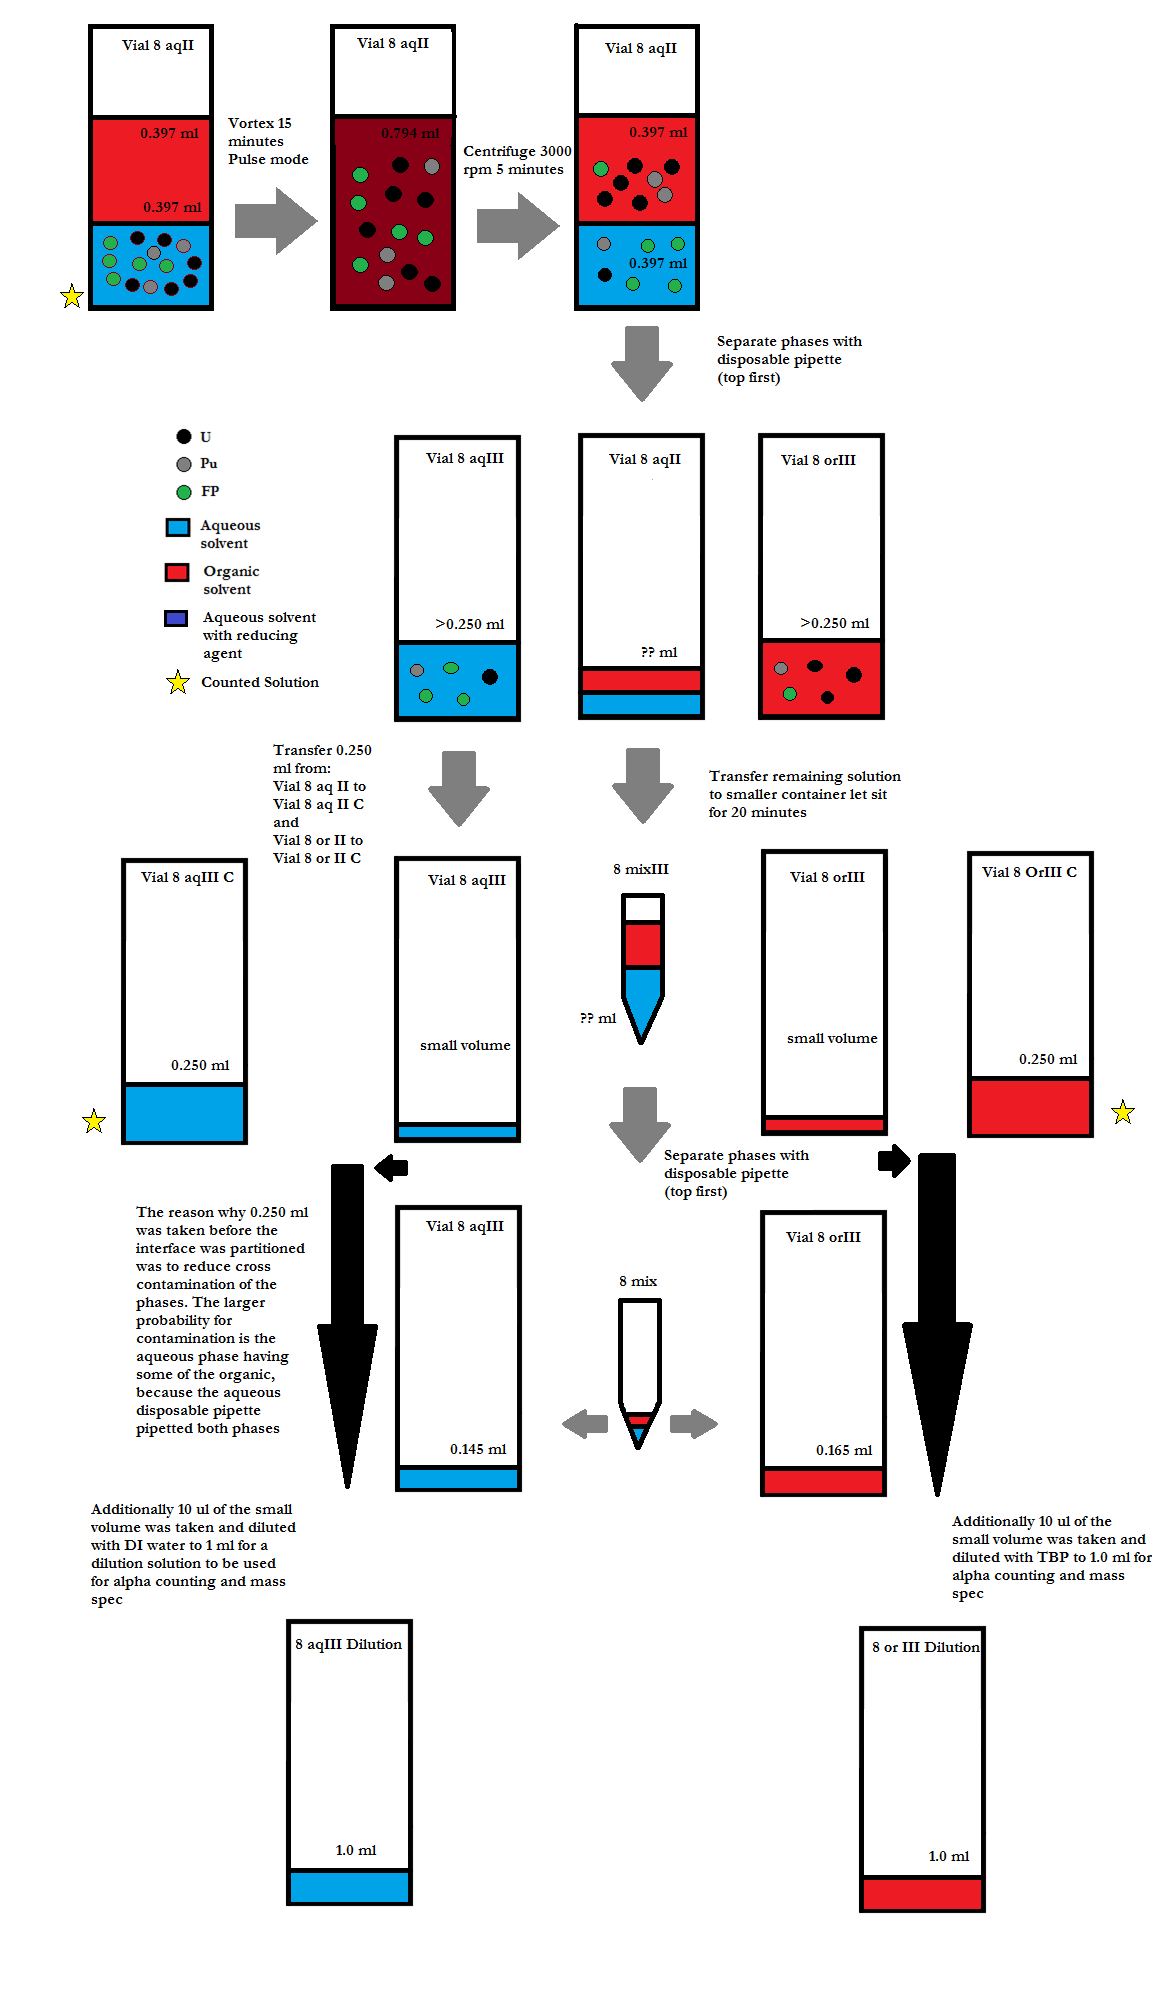
\includegraphics[width=0.8\linewidth]
                  {Figures/Cycle_x3_round_2_extraction_3}
\end{center}
\caption{Extraction three times round 2 extraction 3}
\label{fig:round2_extraction3}
\end{figure}


\experiment{ResearchMeeting}

\begin{itemize}
\item{Email Dr. Burns about the cheat sheet}
\item{Use percentage that Matt used for his paper}
\item{Bug Dr. Folden Friday evening, maybe 1 hour of
enrollment, talk to Julie Zercher look up at CHEM tamu.edu}
\end{itemize}


%-----------------------------------------------------------------
%	LAB BOOK day
%---------------------------------------------------------------

\labday{Thursday 8, December 2016}

\experiment{Process_X3}

\begin{todolist}
\item[\done]{Stop count $\boxed{10\ AqIII\ C}$ $\sim$ 8:30 am}
\item[\done]{Start count $\boxed{8\ OrIII\ C}$ $\sim$ 8:30 am}
\item[\done]{Transfer $\boxed{8\ AqIII\ C}$, $\boxed{9\ AqIII\ C}$,
  $\boxed{10\ AqIII\ C}$ into glove box}
  \begin{itemize}
  \item{In plastic bag (2.5 ml in a 15 ml parafilm wrapped),
    inside the glass beaker - the plastic bag popped
    under the negative pressure and the glass beaker tipped over}
  \item{Centrifuged vials at 2500 rpm for 4 minutes}
  \end{itemize}
\end{todolist}

Fourth contact

\begin{todolist}

\item[\done]{Label vials,
  $\boxed{8\ aqIV}$,
  $\boxed{8\ aqIV\ C}$,  $\boxed{8\ orIV}$,
  $\boxed{8\ orIV\ C}$
  $\boxed{9\ aqIV}$,  $\boxed{9\ aqIV\ C}$,  $\boxed{9\ orIV}$,
  $\boxed{9\ orIV\ C}$
  $\boxed{10\ aqIV}$, $\boxed{10\ aqIV\ C}$, $\boxed{10\ orIV}$,
  $\boxed{10\ orIV\ C}$,
  $\boxed{8\ aqIV\ Dilution}$,
  $\boxed{9\ aqIV\ Dilution}$,
  $\boxed{10\ aqIV\ Dilution}$,
  $\boxed{8\ orIV\ Dilution}$,
  $\boxed{9\ orIV\ Dilution}$,
  $\boxed{10\ orIV\ Dilution}$ (smaller 2.5 ml tubes)
  $\boxed{8\ mixIV}$, $\boxed{9\ mixIV}$,
    $\boxed{10\ mixIV}$ (smaller 1 ml tubes from John Burns,
    have conical bottoms, makes more minute separations easier)}
\item[\done]{Label new vials of old vials...these vials are the
  2.5 ml vials, but have clear push caps that actually fit.
  $\boxed{8\ AqIII}$, $\boxed{9\ AqIII}$, and $\boxed{10\ AqIII}$.}
\item[\done]{Transfer:
  $\boxed{8\ aqIII}$,  $\boxed{8\ aqIII\ C}$,  $\boxed{8\ orIII}$,
  $\boxed{8\ orIII\ C}$
  $\boxed{9\ aqIII}$,  $\boxed{9\ aqIII\ C}$,  $\boxed{9\ orIII}$,
  $\boxed{9\ orIII\ C}$
  $\boxed{10\ aqIII}$, $\boxed{10\ aqIII\ C}$, $\boxed{10\ orIII}$,
  $\boxed{10\ orIII\ C}$,
    $\boxed{8\ aqIII\ Dilution}$,
  $\boxed{9\ aqIII\ Dilution}$,
  $\boxed{10\ aqIII\ Dilution}$,
  $\boxed{8\ orIII\ Dilution}$,
  $\boxed{9\ orIII\ Dilution}$,
  $\boxed{10\ orIII\ Dilution}$,
  $\boxed{8\ mixIII}$, $\boxed{9\ mixIII}$,
  $\boxed{10\ mixIII}$. With old/new $\boxed{8\ AqIII}$, $\boxed{9\ AqIII}$, and $\boxed{10\ AqIII}$.
  (3 clear push caps, and 9 blue push caps
  9 red push caps). With three centrifuge tubes}
\item[\done]{Transfer $\boxed{8\ AqIII\ C}$ + $\boxed{8\ AqIII}$ (old)
     into $\boxed{8\ AqIII}$ (new)}
\item[\done]{Transfer $\boxed{9\ AqIII\ C}$ into $\boxed{9\ AqIII}$ (old)
     into $\boxed{9\ AqIII}$ (new)}
\item[\done]{Transfer $\boxed{10\ AqIII\ C}$ into $\boxed{10\ AqIII}$ (old)
     into $\boxed{10\ AqIII}$ (new)}
\item[\done]{Centrifuge $\boxed{8\ aqIII}$, $\boxed{9\ aqIII}$,
  $\boxed{10\ aqIII}$ for 2,500 rpm. 4 minutes to get liquid to
  bottom}
\item[\done]{Measure volumes of all aqueous phases, $\boxed{8\ aqIII}$
     $\boxed{9\ aqIII}$, $\boxed{10\ aqIII}$}
\begin{table}[H]
  \begin{center}
    \caption{Volumes for combined aqueous phases}
    \begin{tabular}{l l l}
      \toprule
      Series & Aqueous (8,9, or 10)\\ 
      8 & 315+/-3\%\\
      9 & 320+/-3\%\\
      10 & 308+/-3\%\\
      \bottomrule
    \end{tabular}
  \end{center}
\end{table}  
\
\item[\done]{Add 315 $\mu$l of $\boxed{TBP}$ to $\boxed{8\ aqIII}$}
\item[\done]{Add 320 $\mu$l of $\boxed{TBP}$ to $\boxed{9\ aqIII}$}
\item[\done]{Add 308 $\mu$l of $\boxed{TBP}$ to $\boxed{10\ aqIII}$}
\item[\done]{Vortex mix $\boxed{8\ aqIII}$
  for 15 minutes on pulse mode}
\item[\done]{Vortex mix $\boxed{9\ aqIII}$ for 15 minutes on pulse mode}
\item[\done]{Vortex mix $\boxed{10\ aqIII}$ for 15 minutes on pulse mode}

\item[\done]{Centrifuge $\boxed{8\ aqIII}$, $\boxed{9\ aqIII}$,
  and $\boxed{10\ aqIII}$
  with $\boxed{Buddy}$ on 3300 rpm, for 10 minutes}

\item[\done]{Pipette with disposable pipette the organic phase
  first, then the aqueous (for all three vials),
  (also used different disposable pipettes for the
  different phases - no contamination)
  as much as so that there is no mixing.
  Then transferred the boundary to a smaller vial,
  centrifuge, then transfer the rest.
  Prepare counting solutions of 250 $\mu$l of each of the solutions
  A picture will be provided for the whole process for
  $\boxed{8\ aqIII}$
  on the following page
  , also make dilution of each of the phases. Directly below
  are notes for what happened in the initial transfer,
  and below that are notes for the dilution.
  Also consolodated waste after experiment. All interfaces into the
  first mix $\boxed{8\ Mix}$, $\boxed{9\ mix}$, and $\boxed{10\ mix}$,
  also all excess aqueous phase was put into here as well.
  All excess organic (after dilution and creation of count vial, was
  put into a single organic vial $\boxed{8\ Or}$, $\boxed{9\ Or}$,
  and $\boxed{10\ Or}$.)}
  \begin{itemize}
  \item{When transfering interface of $\boxed{8\ AqIII}$ lost a drop}
  \item{Also $\boxed{8\ OrIV\ C}$ might have 248 $\mu$l (less than 250)}
  \item{Same with $\boxed{9\ OrIV\ C}$}
  \end{itemize}
  
\item[\done]{Make dilution of each aqueous}
  \begin{todolist}
  \item[\done]{- $\boxed{8\ aqIV}$}
  \end{todolist}
  \begin{center}
    10+/-0.3 $\mu$l of $\boxed{8\ aqIV}$
    (4 M HNO\tsbs{3}) [smaller pipette]\\
    +\\
    990+/-5.94 $\mu$l of DI water (leftover in glovebox)\\
    =\\
    1.0+/-0.006 ml of $\sim$
    0 M HNO\tsbs{3} $\boxed{8\ aqIV\ Dilution}$
  \end{center}
  \begin{todolist}
  \item[\done]{- $\boxed{9\ aqIV}$}
  \end{todolist}
  \begin{center}
    10+/-0.3 $\mu$l of $\boxed{9\ aqIV}$
    (4 M HNO\tsbs{3}) [smaller pipette]\\
    +\\
    990+/-5.9 $\mu$l of DI water (leftover in glovebox)\\
    =\\
    1.0+/-0.006 ml of $\sim$
    0 M HNO\tsbs{3} $\boxed{9\ aqIV\ Dilution}$
  \end{center}
  \begin{todolist}
  \item[\done]{- $\boxed{10\ aqIV}$}
  \end{todolist}
  \begin{center}
    10+/-0.3 $\mu$l of $\boxed{10\ aqIV}$
    (4 M HNO\tsbs{3}) [smaller pipette]\\
    +\\
    990+/-7.8 $\mu$l of DI water (leftover in glovebox)\\
    =\\
    1.0+/-0.006 ml of $\sim$
    0 M HNO\tsbs{3} $\boxed{10\ aqIV\ Dilution}$
  \end{center}

\item[\done]{Make dilution of each organic phase}
  \begin{todolist}
  \item[\done]{- $\boxed{8\ orIV}$}
  \end{todolist}
  \begin{center}
    10+/-0.3 $\mu$l of $\boxed{8\ orIV}$
    (30\% TBP) [smaller pipette]\\
    +\\
    990+/-7.8 $\mu$l of 30\% TBP (leftover in glovebox)\\
    =\\
    1.0+/-0.006 ml of 30\% TBP $\boxed{8\ orIV\ Dilution}$
  \end{center}
  \begin{todolist}
  \item[\done]{- $\boxed{9\ orIV}$}
  \end{todolist}
  \begin{center}
    10+/-0.3 $\mu$l of $\boxed{9\ orIV}$
    (30\% TBP) [smaller pipette]\\
    +\\
    990+/-7.8 $\mu$l of 30\% TBP (leftover in glovebox)\\
    =\\
    1.0+/-0.006 ml of 30\% TBP $\boxed{9\ orIV\ Dilution}$
  \end{center}
  \begin{todolist}
  \item[\done]{- $\boxed{10\ orIV}$}
  \end{todolist}
  \begin{center}
    10+/-0.3 $\mu$l of $\boxed{10\ orIV}$
    (30\% TBP) [smaller pipette]\\
    +\\
    990+/-7.8 $\mu$l of 30\% TBP (leftover in glovebox)\\
    =\\
    1.0+/-0.006 ml of 30\% TBP $\boxed{10\ orIV\ Dilution}$
  \end{center}
 
\item[\done]{Transfer out $\boxed{8\ orIV\ C}$, $\boxed{8\ aqIV\ C}$,
  $\boxed{9\ orIV\ C}$, $\boxed{9\ aqIV\ C}$, $\boxed{10\ orIV\ C}$,
  $\boxed{10\ aqIV\ C}$, in 15 ml centrifuge tubes}
\item[\done]{Clean stuff in glovebox}
\item[\done]{Radiac wash the above tubes, and store in fumehood behind
  lead - wait to count}
\item[\done]{Centrifuge $\boxed{8\ orIV\ C}$, $\boxed{8\ aqIV\ C}$,
  $\boxed{9\ orIV\ C}$, $\boxed{9\ aqIV\ C}$, $\boxed{10\ orIV\ C}$,
  $\boxed{10\ aqIV\ C}$, for 2 minutes 4,400 rpm to put all liquid at
  bottom, then parafilm wrap all the vials and store in fumehood.}
\item[\done]{Stop count $\boxed{8\ OrIII\ C}$ at 7:30 pm}
\item[\done]{Start count $\boxed{9\ OrIII\ C}$ at 7:30 pm
           (count overnight)} 
\end{todolist}

\begin{figure}[H] % Example of including images
\begin{center}
  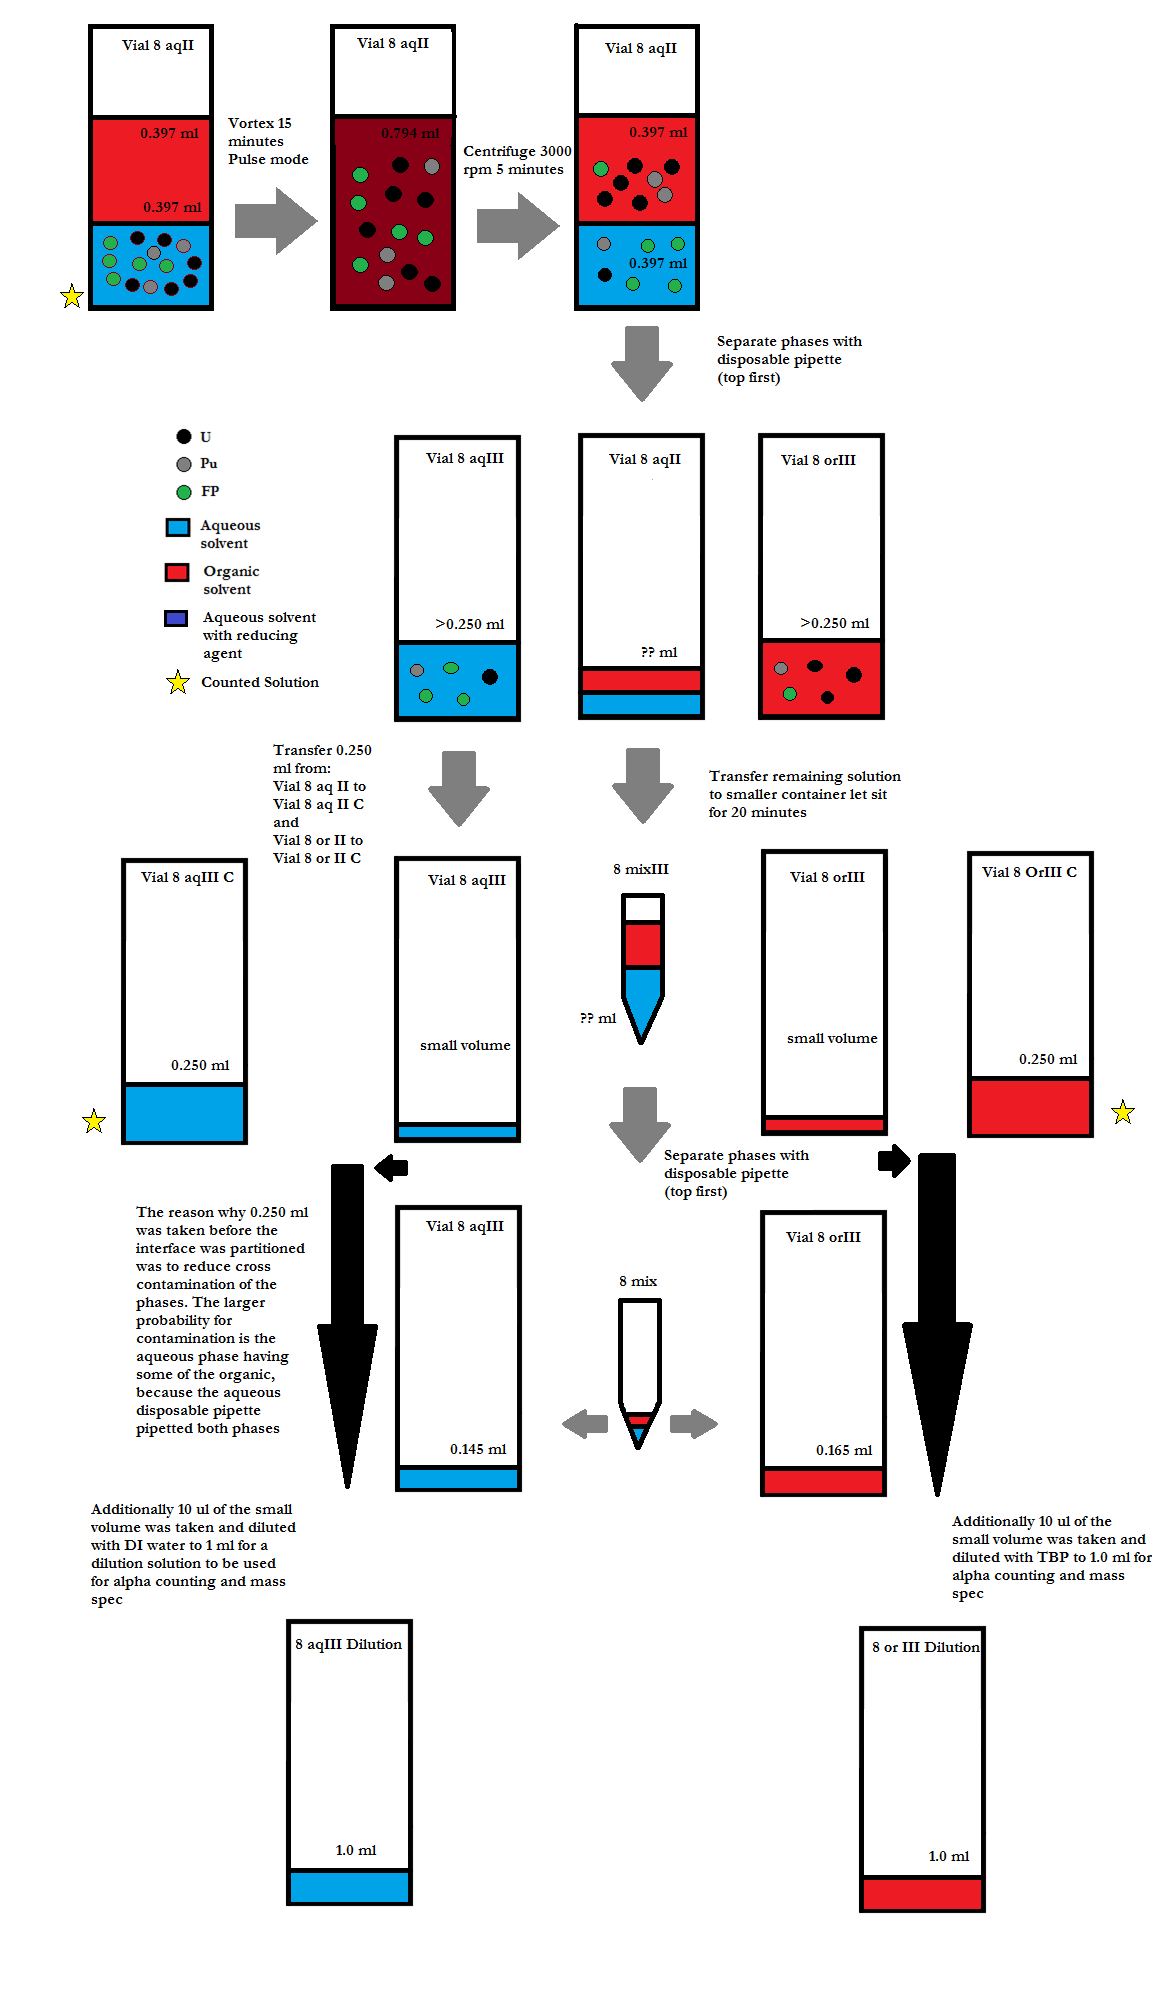
\includegraphics[width=0.8\linewidth]
                  {Figures/Cycle_x3_round_2_extraction_3}
\end{center}
\caption{Extraction three times round 2 extraction 3}
\label{fig:round2_extraction3}
\end{figure}


\experiment{ToCheckout}

\begin{todolist}
\item{Dr. Burns mentioned that Pu-238 overlaps with
  \tss{241}Am in the alpha spec}
\end{todolist}




%-----------------------------------------------------------------
%	LAB BOOK day
%---------------------------------------------------------------

\labday{Friday 9, December 2016}

\experiment{Process_X3}

\begin{todolist}
\item[\done]{Stop count $\boxed{9\ OrIII\ C}$ ($\sim$ 7:20 am)}
\item[\done]{Start count $\boxed{10\ OrIII\ C}$ ($\sim$ 7:20 am)}
\item[\done]{Stop count $\boxed{10\ OrIII\ C}$ (late afternoon)}
\item[\done]{Start count $\boxed{8\ OrIV\ C}$ (late afternoon)}
\end{todolist}

\experiment{School}

\begin{todolist}
\item{Dr. McClarren's homework}
  \begin{itemize}
  \item{This homework...is so long}
  \end{itemize}
\end{todolist}

%-----------------------------------------------------------------
%	LAB BOOK day
%---------------------------------------------------------------

\labday{Satuday 10, December 2016}

\experiment{Process_X3}

\begin{todolist}
\item[\done]{Stop count $\boxed{8\ OrIV\ C}$ (early morning)}
\item[\done]{Start count $\boxed{9\ OrIV\ C}$ (early morning)}
\item[\done]{Stop count $\boxed{9\ OrIV\ C}$ (late afternoon)}
\item[\done]{Start count $\boxed{10\ OrIV\ C}$ (late afternoon)}
\end{todolist}

\experiment{School}

\begin{todolist}
\item{Dr. McClarren's Homework}
  \begin{itemize}
  \item{This homework...is so long}
  \end{itemize}
\end{todolist}


%-----------------------------------------------------------------
%	LAB BOOK day
%---------------------------------------------------------------

\labday{Sunday 11, December 2016}

\experiment{Process_X3}

\begin{todolist}
\item[\done]{Stop count $\boxed{10\ OrIV\ C}$ (early morning)}
\item[\done]{Start count $\boxed{8\ AqIV\ C}$ (early morning)}
\item[\done]{Stop count $\boxed{8\ AqIV\ C}$ (noon)}
\item[\done]{Start count $\boxed{9\ AqIV\ C}$ (noon)}
\item[\done]{Stop count $\boxed{9\ AqIV\ C}$ (afternoon)}
\item[\done]{Start count $\boxed{10\ AqIV\ C}$ (afternoon)}
\item[\done]{Stop count $\boxed{10\ AqIV\ C}$ (late afternoon)}
\end{todolist}


\experiment{School}

\begin{todolist}
\item{Dr. McClarren's Homework}
  \begin{itemize}
  \item{This homework...is so long}
  \end{itemize}
\end{todolist}


%-----------------------------------------------------------------
%	LAB BOOK day
%---------------------------------------------------------------

\labday{Monday 12, December 2016}

\experiment{School}

\begin{todolist}
\item{Dr. McClarren's Homework}
  \begin{itemize}
  \item{This homework...is so long}
  \end{itemize}
\end{todolist}


%-----------------------------------------------------------------
%	LAB BOOK day
%---------------------------------------------------------------

\labday{Tuesday 13, December 2016}

\experiment{School}

\begin{todolist}
\item{Dr. McClarren's Homework}
  \begin{itemize}
  \item{This homework...is so long}
  \end{itemize}
\end{todolist}

%-----------------------------------------------------------------
%	LAB BOOK day
%---------------------------------------------------------------

\labday{Wednesday 14, December 2016}

\experiment{School}

\begin{todolist}
\item[\done]{Dr. McClarren's Homework}
  \begin{itemize}
  \item{This homework...is so long}
  \item{But finally finished, it was 62 pages...}
  \end{itemize}
\end{todolist}


%-----------------------------------------------------------------
%	LAB BOOK day
%---------------------------------------------------------------

\labday{Thursday 15, December 2016}


Prepare for back extraction...

Combine all aqueous,

\begin{todolist}
\item[\done]{Transfer $\boxed{8\ OrIII\ C}$, $\boxed{9\ OrIII\ C}$,
  $\boxed{10\ OrIII\ C}$,
  $\boxed{8\ AqIV\ C}$, $\boxed{9\ AqIV\ C}$,
  $\boxed{10\ AqIV\ C}$,
  $\boxed{8\ OrIV\ C}$, $\boxed{9\ OrIV\ C}$,
  $\boxed{10\ OrIV\ C}$ in plastic bag into the glove box}
\item[\done]{Add $\boxed{8\ AqIII\ C}$ to $\boxed{8\ Mix}$}
\item[\done]{Add $\boxed{9\ AqIII\ C}$ to $\boxed{9\ Mix}$}
\item[\done]{Add $\boxed{10\ AqIII\ C}$ to $\boxed{10\ Mix}$}
  \begin{itemize}
  \item{$\boxed{10\ Mix}$ should be centrifuged next time used}
  \end{itemize}
\end{todolist}

Combine all organic...

\begin{todolist}
\item[\done]{Add $\boxed{8\ OrIII\ C}$ to $\boxed{8\ Or}$}
\item[\done]{Add $\boxed{8\ OrIV\ C}$ to $\boxed{8\ Or}$}
\item[\done]{Add $\boxed{9\ OrIII\ C}$ to $\boxed{9\ Or}$}
\item[\done]{Add $\boxed{9\ OrIV\ C}$ to $\boxed{9\ Or}$}
\item[\done]{Add $\boxed{10\ OrIII\ C}$ to $\boxed{10\ Or}$}
\item[\done]{Add $\boxed{10\ OrIV\ C}$ to $\boxed{10\ Or}$}
\end{todolist}

Create dilution of combined total organic

\begin{todolist}
\item[\done]{Label vials $\boxed{8\ Or\ Tot\ Dilution}$,
  $\boxed{9\ Or\ Tot\ Dilution}$, $\boxed{10\ Or\ Tot\ Dilution}$}
\item[\done]{Transfer $\boxed{8\ Or\ Tot\ Dilution}$,
  $\boxed{9\ Or\ Tot\ Dilution}$, and $\boxed{10\ Or\ Tot\ Dilution}$,
  into glovebox}
\item[\done]{Make dilution of each organic phase}
  \begin{todolist}
  \item[\done]{- $\boxed{8\ or}$}
  \end{todolist}
  \begin{center}
    10+/-0.3 $\mu$l of $\boxed{8\ or}$
    (30\% TBP) [smaller pipette]\\
    +\\
    990+/-7.8 $\mu$l DI water (leftover in glovebox)\\
    =\\
    1.0+/-0.006 ml of DI Water $\boxed{8\ or\ Tot\ Dilution}$
  \end{center}
  \begin{todolist}
  \item[\done]{- $\boxed{9\ or}$}
  \end{todolist}
  \begin{center}
    10+/-0.3 $\mu$l of $\boxed{9\ or}$
    (30\% TBP) [smaller pipette]\\
    +\\
    990+/-7.8 $\mu$l of DI water (leftover in glovebox)\\
    =\\
    1.0+/-0.006 ml of DI water $\boxed{9\ or\ Tot\ Dilution}$
  \end{center}
  \begin{todolist}
  \item[\done]{- $\boxed{10\ or}$}
  \end{todolist}
  \begin{center}
    10+/-0.3 $\mu$l of $\boxed{10\ or}$
    (30\% TBP) [smaller pipette]\\
    +\\
    990+/-7.8 $\mu$l of DI water (leftover in glovebox)\\
    =\\
    1.0+/-0.006 ml of DI water $\boxed{10\ or\ Tot\ Dilution}$
  \end{center}
\end{todolist}

Measure volume of organic

\begin{todolist}
\item[done]{Centrifuge 5 minutes for 2500 rpm $\boxed{8\ or}$,
  $\boxed{9\ or}$, and $\boxed{10\ or}$ with buddy}
\item[\done]{Measure volumes of organics, $\boxed{8\ Or}$
  $\boxed{9\ Or}$, $\boxed{10\ Or}$ (I would guess there
  is probably 1200 $\mu$l in the solution)}
\begin{table}[H]
  \begin{center}
    \caption{Volumes for combined organic phases}
    \begin{tabular}{l l l}
      \toprule
      Series & Organic (8,9, or 10)\\ 
      8 & 888\\
      9 & 912\\
      10 & 863\\
      \bottomrule
    \end{tabular}
  \end{center}
\end{table}  
\end{todolist}
That is much less than what I expected, if this were a perfect world,
there should be 1600 $\mu$l in those vials.

Count the organic phases
\begin{todolist}
\item[\done]{Transfer red lids into glovebox}
\item[\done]{Change clear to red lids on the organic phases}
\item[\done]{Transfer out $\boxed{8\ or}$, $\boxed{9\ or}$,
  $\boxed{10\ or}$ of glovebox, clean, parafilm wrap, centrifuge}
\item[\done]{Start count $\boxed{8\ Or}$ at 0 cm around 11:00 am,
  there is a 5\% dead time, which is about what was
  expected}
\item[\done]{Stop count $\boxed{8\ Or}$ at 0 cm (2:20 pm)}
\item[\done]{Start count $\boxed{9\ Or}$ at 0 cm (2:20 pm)}
\item[\done]{Stop count $\boxed{9\ Or}$ at 0 cm (5:20 pm)}
\item[\done]{Start count $\boxed{10\ Or}$ at 0 cm (5:20 pm) - leave over night}
\end{todolist}

Prepare for the next few days
\begin{todolist}
\item[\done]{Write procedure for back extractions}
\item{Analyze results from previous extractions}
  \begin{itemize}
  \item[\done]{Extraction 3, extraction 4}
  \item{ reanalyze alpha results with
    what Dr. Burns mentioned, write script to minimize variance
    of results varying parameters like volume (not really)}
  \end{itemize}
\item[\done]{Look at homework for 629}
\end{todolist}


%-----------------------------------------------------------------
%	LAB BOOK day
%---------------------------------------------------------------

\labday{Friday 16, December 2016}

\experiment{Process_X3}

Counting

\begin{todolist}
\item[\done]{Stop count $\boxed{10\ Or}$ at 0 cm}
\item[\done]{Transfer $\boxed{8\ Or}$, $\boxed{9 \ Or}$, and $\boxed{10\ Or}$
  into glove box}
\end{todolist}

\textbf{Back extraction experiment 1.}
\textbf{Note }$\bm{\boxed{B}}$\textbf{ is for back extraction.}
\textbf{Also special vials labeled below are the vials with clear push caps
that actually make a good seal.}

\begin{todolist}
\item[\done]{Label vials,
  $\boxed{8\ aqB}$,
  $\boxed{8\ aqB\ C}$,  $\boxed{8\ orB}$ (special) \smiley,
  $\boxed{8\ orB\ C}$
  $\boxed{9\ aqB}$,  $\boxed{9\ aqB\ C}$,  $\boxed{9\ orB}$ (special),
  $\boxed{9\ orB\ C}$
  $\boxed{10\ aqB}$, $\boxed{10\ aqB\ C}$, $\boxed{10\ orB}$ (special),
  $\boxed{10\ orB\ C}$,
  $\boxed{8\ aqB\ Dilution}$,
  $\boxed{9\ aqB\ Dilution}$,
  $\boxed{10\ aqB\ Dilution}$,
  $\boxed{8\ orB\ Dilution}$,
  $\boxed{9\ orB\ Dilution}$,
  $\boxed{10\ orB\ Dilution}$ (smaller 2.5 ml tubes)
  $\boxed{8\ mixB}$, $\boxed{9\ mixB}$,
    $\boxed{10\ mixB}$ (smaller 1 ml tubes from John Burns,
    have conical bottoms, makes more minute separations easier)}

\item[\done]{Transfer:
  $\boxed{8\ aqB}$,
  $\boxed{8\ aqB\ C}$,  $\boxed{8\ orB}$ (special) \smiley,
  $\boxed{8\ orB\ C}$
  $\boxed{9\ aqB}$,  $\boxed{9\ aqB\ C}$,  $\boxed{9\ orB}$ (special),
  $\boxed{9\ orB\ C}$
  $\boxed{10\ aqB}$, $\boxed{10\ aqB\ C}$, $\boxed{10\ orB}$,
  $\boxed{10\ orB\ C}$,
  $\boxed{8\ aqB\ Dilution}$,
  $\boxed{9\ aqB\ Dilution}$,
  $\boxed{10\ aqB\ Dilution}$,
  $\boxed{8\ orB\ Dilution}$,
  $\boxed{9\ orB\ Dilution}$,
  $\boxed{10\ orB\ Dilution}$ (smaller 2.5 ml tubes)
  $\boxed{8\ mixB}$, $\boxed{9\ mixB}$,
    $\boxed{10\ mixB}$ with
  (3 clear push caps, and 12 blue push caps
  6 red push caps) into glovebox in large plastic bag}

\item[\done]{Remember volumes of organic phases, $\boxed{8\ or}$
     $\boxed{9\ or}$, $\boxed{10\ or}$}
\begin{table}[H]
  \begin{center}
    \caption{Volumes for combined organic phases}
    \begin{tabular}{l l l}
      \toprule
      Series & Organic (8,9, or 10)\\ 
      8 & 888\\
      9 & 912\\
      10 & 863\\
      \bottomrule
    \end{tabular}
  \end{center}
\end{table}  
\end{todolist}


Create an Fe solution for a back extraction, $\boxed{Fe\ Prep}$
(Small portions created right before the experiment because this
solution has a short half life with larger concentrations of $HNO_3$).

\begin{todolist}
\item[\done]{-}
\end{todolist}
\begin{center}
0.0417+/-0.0018 ml of 2.302+/-0.009 M Fe(II) in 0.0+/-0 M HNO\tsbs{3} $\boxed{Stock\ Fe(II)}$\\
+\\
3.941+/-0.027 ml of 0.0+/-0 M Fe(II) in 4.06+/-0.05 M HNO\tsbs{3} solution $\boxed{Fe\ Prep}$\\
+\\
4.000+/-0.020 ml of 0.0240+/-0.0010 M Fe(II) in 4.00+/-0.05 M HNO\tsbs{3} solution $\boxed{\rightarrow Bk\ Ex\ Solution}$.
\end{center}

\textbf{Actual Back extraction}

\begin{todolist}
\item[\done]{Add 888 $\mu$l of $\boxed{\rightarrow Bk\ Ex\ Solution}$
  to $\boxed{8\ or}$}
\item[\done]{Add 912 $\mu$l of $\boxed{\rightarrow Bk\ Ex\ Solution}$
  to $\boxed{9\ or}$}
\item[\done]{Add 863 $\mu$l of $\boxed{\rightarrow Bk\ Ex\ Solution}$
  to $\boxed{10\ or}$}
\item[\done]{Vortex mix $\boxed{8\ or}$
  for 15 minutes on pulse mode}
\item[\done]{Vortex mix $\boxed{9\ or}$ for 15 minutes on pulse mode}
\item[\done]{Vortex mix $\boxed{10\ or}$ for 15 minutes on pulse mode}

\item[\done]{Centrifuge $\boxed{8\ or}$, $\boxed{9\ or}$,
  and $\boxed{10\ or}$
  with $\boxed{Buddy}$ on 3300 rpm, for 10 minutes}

\item[\done]{Pipette with disposable pipette the organic phase
  first, then the aqueous (for all three vials),
  (also used different disposable pipettes for the
  different phases - no contamination)
  as much as so that there is no mixing.
  Then transferred the boundary to a smaller vial,
  centrifuge (3,300 for $\sim$ 5 minutes), then transfer the rest.
  Prepare counting solutions of 500 $\mu$l of each of the solutions
  A picture will be provided for the whole process for
  some step for series 8,
  on the following page (picture is of a previous experiment,
  but same process)
  , also make dilution of each of the phases. Directly below
  are notes for what happened in the initial transfer,
  and below that are notes for the dilution.}
  \begin{itemize}
  \item{Did pretty well this time around}
  \end{itemize}
  
\item[\done]{Make dilution of each aqueous}
  \begin{todolist}
  \item[\done]{- $\boxed{8\ aqB}$}
  \end{todolist}
  \begin{center}
    10+/-0.3 $\mu$l of $\boxed{8\ aqB}$
    (4 M HNO\tsbs{3}) [smaller pipette]\\
    +\\
    990+/-5.94 $\mu$l of DI water (leftover in glovebox)\\
    =\\
    1.0+/-0.006 ml of $\sim$
    0 M HNO\tsbs{3} $\boxed{8\ aqB\ Dilution}$
  \end{center}
  \begin{todolist}
  \item[\done]{- $\boxed{9\ aqB}$}
  \end{todolist}
  \begin{center}
    10+/-0.3 $\mu$l of $\boxed{9\ aqB}$
    (4 M HNO\tsbs{3}) [smaller pipette]\\
    +\\
    990+/-5.9 $\mu$l of DI water (leftover in glovebox)\\
    =\\
    1.0+/-0.006 ml of $\sim$
    0 M HNO\tsbs{3} $\boxed{9\ aqB\ Dilution}$
  \end{center}
  \begin{todolist}
  \item[\done]{- $\boxed{10\ aqB}$}
  \end{todolist}
  \begin{center}
    10+/-0.3 $\mu$l of $\boxed{10\ aqB}$
    (4 M HNO\tsbs{3}) [smaller pipette]\\
    +\\
    990+/-7.8 $\mu$l of DI water (leftover in glovebox)\\
    =\\
    1.0+/-0.006 ml of $\sim$
    0 M HNO\tsbs{3} $\boxed{10\ aqB\ Dilution}$
  \end{center}

\item[\done]{Make dilution of each organic phase}
  \begin{todolist}
  \item[\done]{- $\boxed{8\ orB}$}
  \end{todolist}
  \begin{center}
    10+/-0.3 $\mu$l of $\boxed{8\ orB}$
    (30\% TBP) [smaller pipette]\\
    +\\
    990+/-7.8 $\mu$l of DI water (leftover in glovebox)\\
    =\\
    1.0+/-0.006 ml of DI water $\boxed{8\ orB\ Dilution}$
  \end{center}
  \begin{todolist}
  \item[\done]{- $\boxed{9\ orB}$}
  \end{todolist}
  \begin{center}
    10+/-0.3 $\mu$l of $\boxed{9\ orB}$
    (30\% TBP) [smaller pipette]\\
    +\\
    990+/-7.8 $\mu$l of DI water (leftover in glovebox)\\
    =\\
    1.0+/-0.006 ml of DI water $\boxed{9\ orB\ Dilution}$
  \end{center}
  \begin{todolist}
  \item[\done]{- $\boxed{10\ orB}$}
  \end{todolist}
  \begin{center}
    10+/-0.3 $\mu$l of $\boxed{10\ orB}$
    (30\% TBP) [smaller pipette]\\
    +\\
    990+/-7.8 $\mu$l of DI water (leftover in glovebox)\\
    =\\
    1.0+/-0.006 ml of DI water $\boxed{10\ orB\ Dilution}$
  \end{center}
 
\item[\done]{Transfer out $\boxed{8\ orB\ C}$, $\boxed{8\ aqB\ C}$,
  $\boxed{9\ orB\ C}$, $\boxed{9\ aqB\ C}$, $\boxed{10\ orB\ C}$,
  $\boxed{10\ aqB\ C}$, in 15 ml centrifuge tubes}
\item[\done]{Clean stuff in glovebox}
\item[\done]{Radiac wash the above tubes, and store in fumehood behind
  lead - wait to count}
\item[\done]{Centrifuge $\boxed{8\ orB\ C}$, $\boxed{8\ aqB\ C}$,
  $\boxed{9\ orB\ C}$, $\boxed{9\ aqB\ C}$, $\boxed{10\ orB\ C}$,
  $\boxed{10\ aqB\ C}$, for 2 minutes 4,400 rpm to put all liquid at
  bottom, then parafilm wrap all the vials and store in fumehood.}
\item[\done]{Start count $\boxed{8\ OrB\ C}$ at 12:36 pm} 
\end{todolist}

\begin{figure}[H] % Example of including images
\begin{center}
  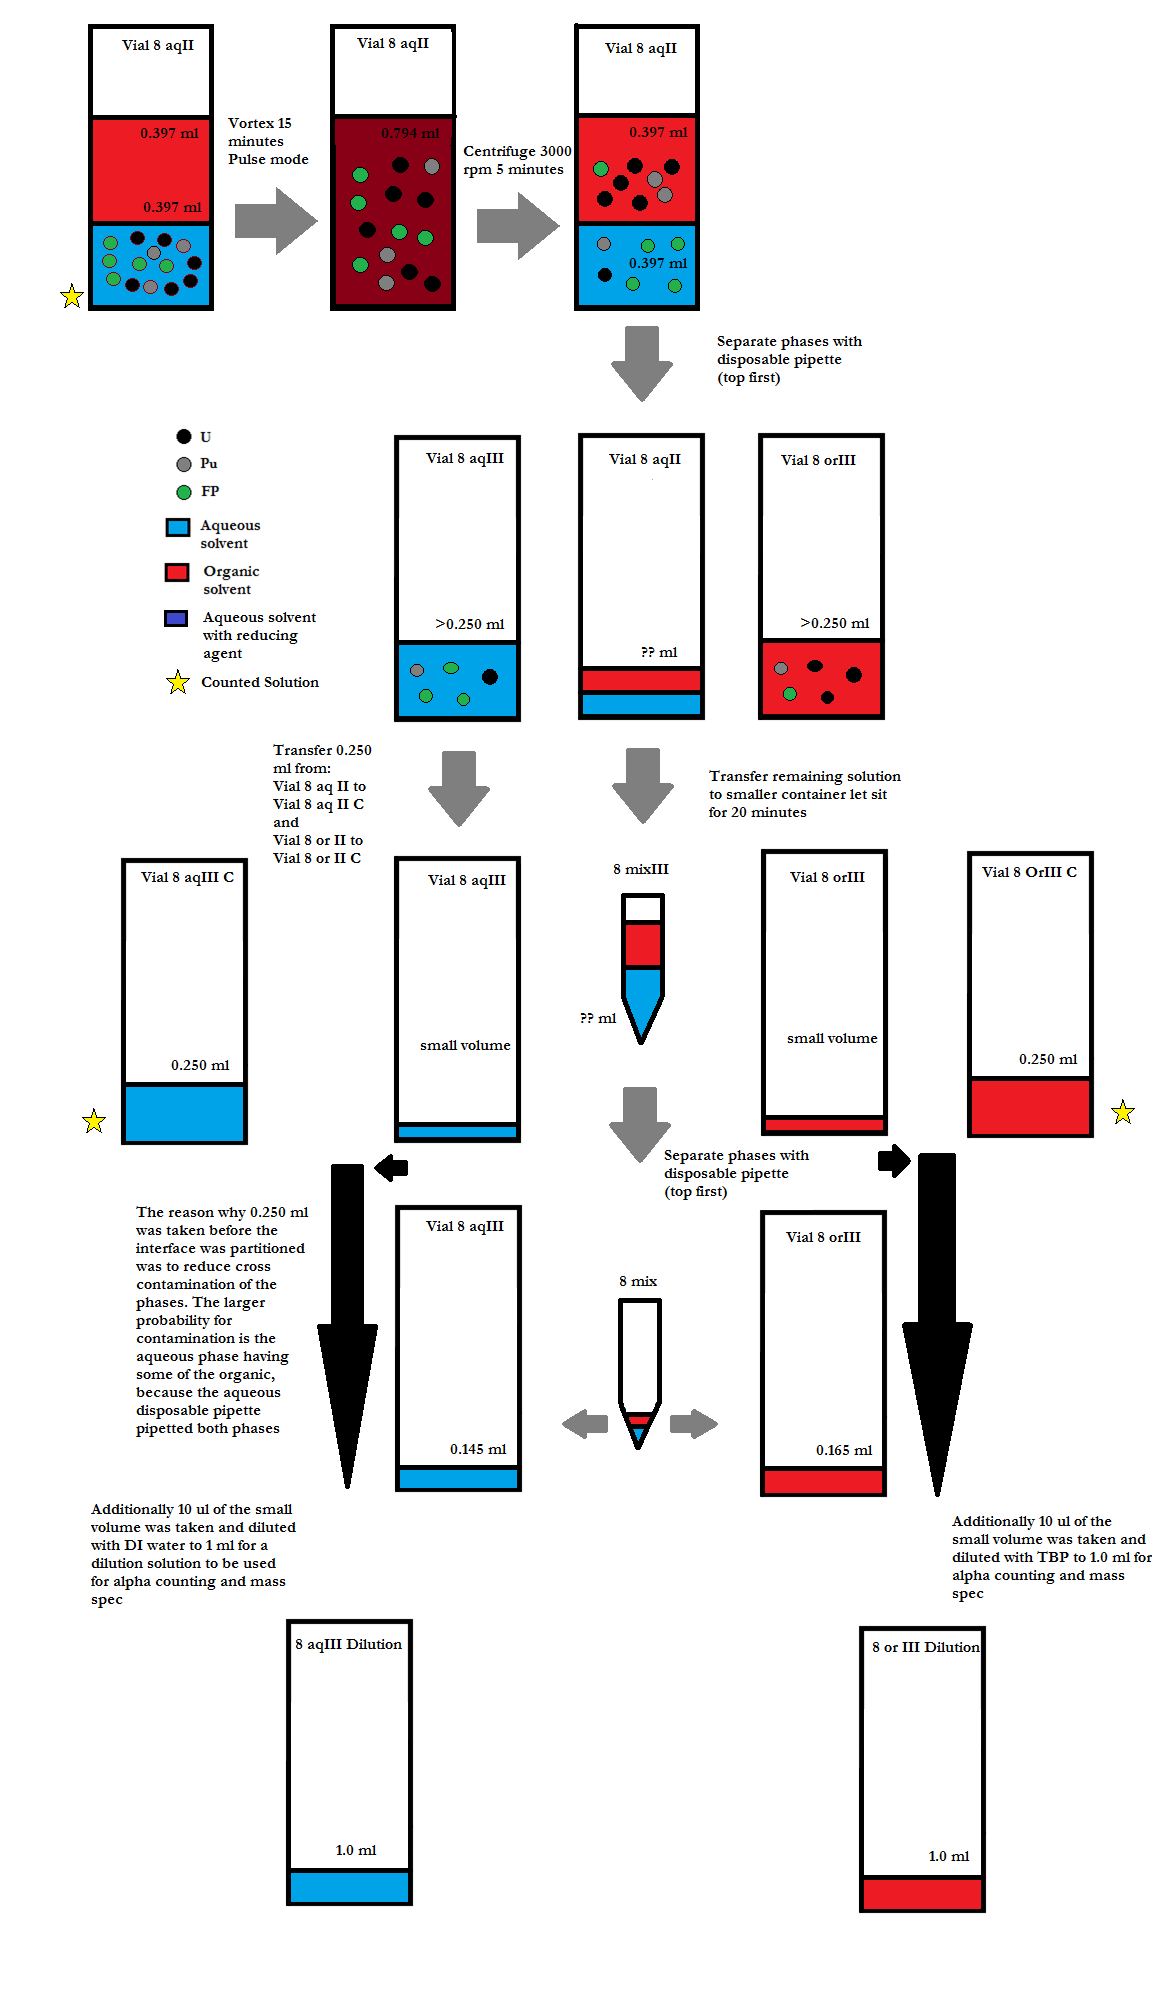
\includegraphics[width=0.8\linewidth]
                  {Figures/Cycle_x3_round_2_extraction_3}
\end{center}
\caption{Back extraction I, (different vial names, same procedure)}
\label{fig:round2_extraction3}
\end{figure}



\begin{todolist}
\item[\done]{Write up procedure for weekend and Monday}
\end{todolist}



\experiment{Buy}
I kind of don't want to ask for this because anytime money comes
up with Dr. Chirayath he gets really rude and mean.
\begin{todolist}
\item{500, 15 ml centrifuge tubes from VWR, catalog \# 89401-574
  priced at \$302.98}
\end{todolist}


\experiment{Process_X3}
\begin{todolist}
\item[\done]{Prepare for second back extraction}
\item[\done]{Stop count $\boxed{8\ OrB\ C}$ at 12:36 am}
\item[\done]{Start count $\boxed{9\ OrB\ C}$ at 12:36 am} 
\end{todolist}

%-----------------------------------------------------------------
%	LAB BOOK day
%---------------------------------------------------------------

\labday{Saturday 17, December 2016}

\experiment{Process_X3}

\textbf{Counting}
\begin{todolist}
\item[\done]{Stop count $\boxed{9\ OrB\ C}$ at 12:36 pm}
\item[\done]{Start count $\boxed{10\ OrB\ C}$ at 12:36 pm}
\end{todolist}


%-----------------------------------------------------------------
%	LAB BOOK day
%---------------------------------------------------------------

\labday{Sunday 18, December 2016}

\experiment{Process_X3}

\textbf{Counting}
\begin{todolist}
\item[\done]{Stop count $\boxed{10\ OrB\ C}$ at 8:00 am}
\item[\done]{Start count $\boxed{8\ AqB\ C}$ at 8:00 am}
\item[\done]{Stop count $\boxed{8\ AqB\ C}$ at 5:00 pm}
\item[\done]{Start count $\boxed{9\ AqB\ C}$ at 5:00 pm}
\item[\done]{Stop count $\boxed{9\ AqB\ C}$ at 10:00 pm}
\item[\done]{Start count $\boxed{8\ OrBII\ C}$ at 10:00 pm (from experiment
  desribed tomorrow (I did it on Sunday afternoon to get more
count time)}
\end{todolist}

%-----------------------------------------------------------------
%	LAB BOOK day
%---------------------------------------------------------------

\labday{Monday 19, December 2016}

\experiment{Process_X3}

\textbf{Counting}
\begin{todolist}
\item[\done]{Stop count $\boxed{8\ OrBII\ C}$ at 11:00 am}
\item[\done]{Start count $\boxed{9\ OrBII\ C}$ at 11:00 am}
\end{todolist}


\textbf{Prepare for second back extraction}
\begin{todolist}
\item[\done]{Transfer into glovebox $\boxed{8\ orB\ C}$,
  $\boxed{9\ orB\ C}$, $\boxed{10\ orB\ C}$,
  in 15 ml centrifuge tubes, parafilm wrapped, in plastic bag}
\item[\done]{Label vials,
  $\boxed{8\ aqBII}$,
  $\boxed{8\ aqBII\ C}$,  $\boxed{8\ orBII}$ (special) \smiley,
  $\boxed{8\ orBII\ C}$
  $\boxed{9\ aqBII}$,
  $\boxed{9\ aqBII\ C}$,  $\boxed{9\ orBII}$ (special),
  $\boxed{9\ orBII\ C}$
  $\boxed{10\ aqBII}$, $\boxed{10\ aqBII\ C}$,
  $\boxed{10\ orBII}$ (special),
  $\boxed{10\ orBII\ C}$,
  $\boxed{8\ aqBII\ Dilution}$,
  $\boxed{9\ aqBII\ Dilution}$,
  $\boxed{10\ aqBII\ Dilution}$,
  $\boxed{8\ orBII\ Dilution}$,
  $\boxed{9\ orBII\ Dilution}$,
  $\boxed{10\ orBII\ Dilution}$ (smaller 2.5 ml tubes)
  $\boxed{8\ mixBII}$, $\boxed{9\ mixBII}$,
    $\boxed{10\ mixBII}$ (smaller 1 ml tubes from John Burns,
    have conical bottoms, makes more minute separations easier)}

\item[\done]{Transfer:   $\boxed{8\ aqBII}$,
  $\boxed{8\ aqBII\ C}$,  $\boxed{8\ orBII}$ (special) \smiley,
  $\boxed{8\ orBII\ C}$
  $\boxed{9\ aqBII}$,
  $\boxed{9\ aqBII\ C}$,  $\boxed{9\ orBII}$ (special),
  $\boxed{9\ orBII\ C}$
  $\boxed{10\ aqBII}$, $\boxed{10\ aqBII\ C}$,
  $\boxed{10\ orBII}$ (special),
  $\boxed{10\ orBII\ C}$,
  $\boxed{8\ aqBII\ Dilution}$,
  $\boxed{9\ aqBII\ Dilution}$,
  $\boxed{10\ aqBII\ Dilution}$,
  $\boxed{8\ orBII\ Dilution}$,
  $\boxed{9\ orBII\ Dilution}$,
  $\boxed{10\ orBII\ Dilution}$ (smaller 2.5 ml tubes)
  $\boxed{8\ mixBII}$, $\boxed{9\ mixBII}$,
    $\boxed{10\ mixBII}$
  with
  (3 clear push caps, and 12 blue push caps
  3 red push caps) into glovebox in large plastic bag}
\end{todolist}
\textbf{Combine all organic phases}

\begin{todolist}  
\item[\done]{Transfer $\boxed{8\ OrB\ C}$ into $\boxed{8\ OrB}$}
\item[\done]{Transfer $\boxed{9\ OrB\ C}$ into $\boxed{9\ OrB}$}
\item[\done]{Transfer $\boxed{10\ OrB\ C}$ into $\boxed{10\ OrB}$}
\end{todolist}
  
\textbf{\st{Combine all aqueous phases (still counting)}}
\begin{todolist}
\item{Transfer $\boxed{8\ AqB\ C}$ into $\boxed{8\ AqB}$}
\item{Transfer $\boxed{9\ AqB\ C}$ into $\boxed{9\ AqB}$}
\item{Transfer $\boxed{10\ AqB\ C}$ into $\boxed{10\ AqB}$}
\end{todolist}

\textbf{Measure volume of organic phases}
\begin{todolist}
\item[\done]{Centrifuge $\boxed{8\ OrB}$, $\boxed{9\ OrB}$,
  $\boxed{10\ OrB}$ for 2,500 rpm. 4 minutes to get liquid to
  bottom}
\item[\done]{Measure volumes of all organic phases, $\boxed{8\ OrB}$
     $\boxed{9\ OrB}$, $\boxed{10\ OrB}$}
\begin{table}[H]
  \begin{center}
    \caption{Volumes for combined organic phases}
    \begin{tabular}{l l l}
      \toprule
      Series & Organic (8,9, or 10)\\ 
      8 & 760\\
      9 & 765\\
      10 & 770\\
      \bottomrule
    \end{tabular}
  \end{center}
\end{table}  
\end{todolist}

Create an Fe solution for a back extraction, $\boxed{Fe\ Prep}$
(Small portions created right before the experiment because this
solution has a short half life with larger concentrations of $HNO_3$).

\begin{todolist}
\item[\done]{-}
\end{todolist}
\begin{center}
0.0417+/-0.0018 ml of 2.302+/-0.009 M Fe(II) in 0.0+/-0 M HNO\tsbs{3} $\boxed{Stock\ Fe(II)}$\\
+\\
3.941+/-0.027 ml of 0.0+/-0 M Fe(II) in 4.06+/-0.05 M HNO\tsbs{3} solution $\boxed{Fe\ Prep}$\\
+\\
4.000+/-0.020 ml of 0.0240+/-0.0010 M Fe(II) in 4.00+/-0.05 M HNO\tsbs{3} solution $\boxed{\rightarrow Bk\ Ex\ Solution}$.
\end{center}

\textbf{Actual Back extraction}

\begin{todolist}
\item[\done]{Add 760 $\mu$l of $\boxed{\rightarrow Bk\ Ex\ Solution}$
  to $\boxed{8\ orB}$}
\item[\done]{Add 765 $\mu$l of $\boxed{\rightarrow Bk\ Ex\ Solution}$
  to $\boxed{9\ orB}$}
\item[\done]{Add 770 $\mu$l of $\boxed{\rightarrow Bk\ Ex\ Solution}$
  to $\boxed{10\ orB}$}
\item[\done]{Vortex mix $\boxed{8\ orB}$
  for 15 minutes on pulse mode}
\item[\done]{Vortex mix $\boxed{9\ orB}$ for 15 minutes on pulse mode}
\item[\done]{Vortex mix $\boxed{10\ orB}$ for 15 minutes on pulse mode}

\item[\done]{Centrifuge $\boxed{8\ orB}$, $\boxed{9\ orB}$,
  and $\boxed{10\ orB}$
  with $\boxed{Buddy}$ on 3300 rpm, for 10 minutes}

\item[\done]{Pipette with disposable pipette the organic phase
  first, then the aqueous (for all three vials),
  (also used different disposable pipettes for the
  different phases - no contamination)
  as much as so that there is no mixing.
  Then transferred the boundary to a smaller vial,
  centrifuge, then transfer the rest.
  Prepare counting solutions of 500 $\mu$l of each of the solutions
  A picture will be provided for the whole process for
  some step for series 8,
  on the following page (picture is of a previous experiment,
  but same process)
  , also make dilution of each of the phases. Directly below
  are notes for what happened in the initial transfer,
  and below that are notes for the dilution. Also after
  dilution and counting solutions are made, combine all remaining
  aqueous solution into $\boxed{8\ aqB}$, $\boxed{9\ aqB}$,
  or $\boxed{10\ aqB}$. }
  \begin{itemize}
  \item{$\boxed{10\ AqBII\ C}$ probably doesn't have 500 $\mu$l
  maybe 480-495}
  \end{itemize}
  
\item[\done]{Make dilution of each aqueous}
  \begin{todolist}
  \item[\done]{- $\boxed{8\ aqBII}$}
  \end{todolist}
  \begin{center}
    10+/-0.3 $\mu$l of $\boxed{8\ aqBII}$
    (4 M HNO\tsbs{3}) [smaller pipette]\\
    +\\
    990+/-5.94 $\mu$l of DI water (leftover in glovebox)\\
    =\\
    1.0+/-0.006 ml of $\sim$
    0 M HNO\tsbs{3} $\boxed{8\ aqBII\ Dilution}$
  \end{center}
  \begin{todolist}
  \item[\done]{- $\boxed{9\ aqBII}$}
  \end{todolist}
  \begin{center}
    10+/-0.3 $\mu$l of $\boxed{9\ aqBII}$
    (4 M HNO\tsbs{3}) [smaller pipette]\\
    +\\
    990+/-5.9 $\mu$l of DI water (leftover in glovebox)\\
    =\\
    1.0+/-0.006 ml of $\sim$
    0 M HNO\tsbs{3} $\boxed{9\ aqBII\ Dilution}$
  \end{center}
  \begin{todolist}
  \item[\done]{- $\boxed{10\ aqBII}$}
  \end{todolist}
  \begin{center}
    10+/-0.3 $\mu$l of $\boxed{10\ aqBII}$
    (4 M HNO\tsbs{3}) [smaller pipette]\\
    +\\
    990+/-7.8 $\mu$l of DI water (leftover in glovebox)\\
    =\\
    1.0+/-0.006 ml of $\sim$
    0 M HNO\tsbs{3} $\boxed{10\ aqBII\ Dilution}$
  \end{center}

\item[\done]{Make dilution of each organic phase}
  \begin{todolist}
  \item[\done]{- $\boxed{8\ orBII}$}
  \end{todolist}
  \begin{center}
    10+/-0.3 $\mu$l of $\boxed{8\ orBII}$
    (30\% TBP) [smaller pipette]\\
    +\\
    990+/-7.8 $\mu$l of DI water (leftover in glovebox)\\
    =\\
    1.0+/-0.006 ml of DI water $\boxed{8\ orBII\ Dilution}$
  \end{center}
  \begin{todolist}
  \item[\done]{- $\boxed{9\ orBII}$}
  \end{todolist}
  \begin{center}
    10+/-0.3 $\mu$l of $\boxed{9\ orBII}$
    (30\% TBP) [smaller pipette]\\
    +\\
    990+/-7.8 $\mu$l of DI water (leftover in glovebox)\\
    =\\
    1.0+/-0.006 ml of DI water $\boxed{9\ orBII\ Dilution}$
  \end{center}
  \begin{todolist}
  \item[\done]{- $\boxed{10\ orBII}$}
  \end{todolist}
  \begin{center}
    10+/-0.3 $\mu$l of $\boxed{10\ orBII}$
    (30\% TBP) [smaller pipette]\\
    +\\
    990+/-7.8 $\mu$l of DI water (leftover in glovebox)\\
    =\\
    1.0+/-0.006 ml of DI water $\boxed{10\ orBII\ Dilution}$
  \end{center}
 
\item[\done]{Transfer out $\boxed{8\ orBII\ C}$, $\boxed{8\ aqBII\ C}$,
  $\boxed{9\ orBII\ C}$, $\boxed{9\ aqBII\ C}$, $\boxed{10\ orBII\ C}$,
  $\boxed{10\ aqBII\ C}$, in 15 ml centrifuge tubes}
\item{Clean stuff in glovebox}
\item[\done]{Radiac wash the above tubes, and store in fumehood behind
  lead - wait to count}
\item[\done]{Centrifuge $\boxed{8\ orBII\ C}$, $\boxed{8\ aqBII\ C}$,
  $\boxed{9\ orBII\ C}$, $\boxed{9\ aqBII\ C}$, $\boxed{10\ orBII\ C}$,
  $\boxed{10\ aqBII\ C}$, for 2 minutes 4,400 rpm to put all liquid at
  bottom, then parafilm wrap all the vials and store in fumehood.}
\end{todolist}
\textbf{Counting}
\begin{todolist}
\item[\done]{Stop count $\boxed{9\ OrBII\ C}$ around 10:00 pm}
\item[\done]{Start count $\boxed{10\ OrBII\ C}$ around 10:00pm}
\end{todolist}

\begin{figure}[H] % Example of including images
\begin{center}
  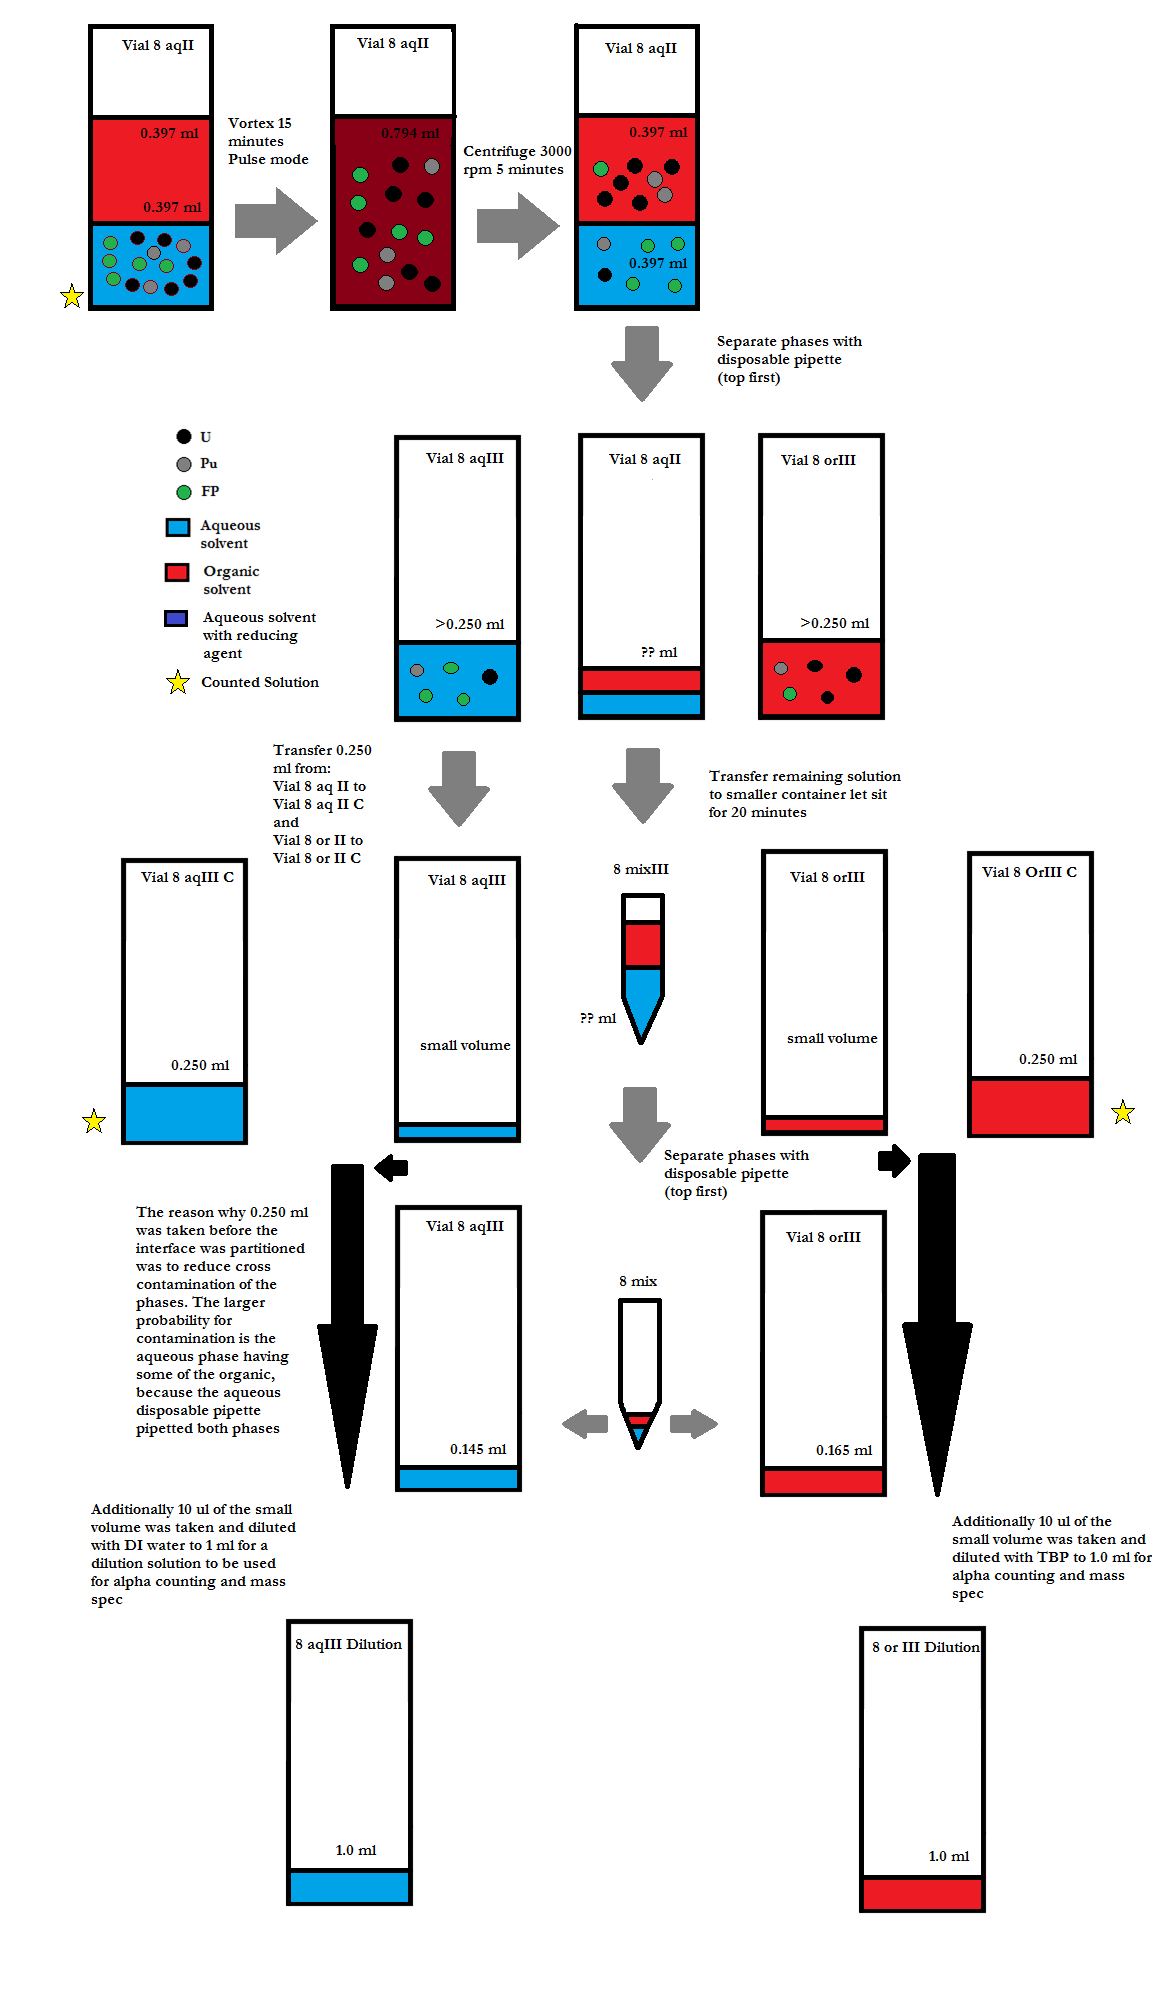
\includegraphics[width=0.8\linewidth]
                  {Figures/Cycle_x3_round_2_extraction_3}
\end{center}
\caption{Back extraction I, (different vial names, same procedure)}
\label{fig:round2_extraction3}
\end{figure}





%-----------------------------------------------------------------
%	LAB BOOK day
%---------------------------------------------------------------

\labday{Tuesday 20, December 2016}

\experiment{Process_X3}

\textbf{Counting}
\begin{todolist}
\item[\done]{Stop count for $\boxed{10\ OrBII\ C}$}
\item[\done]{Start count for $\boxed{10\ AqB\ C}$ (finish out
back extraction aqueous counts)}
\end{todolist}

\textbf{Prepare for third back extraction}
\begin{todolist}
\item[\done]{Transfer into glovebox $\boxed{8\ orBII\ C}$,
  $\boxed{9\ orBII\ C}$, $\boxed{10\ orBII\ C}$,
  in 15 ml centrifuge tubes, parafilm wrapped, in plastic bag}
\item[\done]{Label vials,
  $\boxed{8\ aqBIII}$,
  $\boxed{8\ aqBIII\ C}$,  $\boxed{8\ orBIII}$ (special) \smiley,
  $\boxed{8\ orBIII\ C}$
  $\boxed{9\ aqBIII}$,
  $\boxed{9\ aqBIII\ C}$,  $\boxed{9\ orBIII}$ (special),
  $\boxed{9\ orBIII\ C}$
  $\boxed{10\ aqBIII}$, $\boxed{10\ aqBIII\ C}$,
  $\boxed{10\ orBIII}$ (special),
  $\boxed{10\ orBIII\ C}$,
  $\boxed{8\ aqBIII\ Dilution}$,
  $\boxed{9\ aqBIII\ Dilution}$,
  $\boxed{10\ aqBIII\ Dilution}$,
  $\boxed{8\ orBIII\ Dilution}$,
  $\boxed{9\ orBIII\ Dilution}$,
  $\boxed{10\ orBIII\ Dilution}$ (smaller 2.5 ml tubes)
  $\boxed{8\ mixBIII}$, $\boxed{9\ mixBIII}$,
    $\boxed{10\ mixBIII}$ (smaller 1 ml tubes from John Burns,
    have conical bottoms, makes more minute separations easier)}

\item[\done]{Transfer:   $\boxed{8\ aqBIII}$,
  $\boxed{8\ aqBIII\ C}$,  $\boxed{8\ orBIII}$ (special) \smiley,
  $\boxed{8\ orBIII\ C}$
  $\boxed{9\ aqBIII}$,
  $\boxed{9\ aqBIII\ C}$,  $\boxed{9\ orBIII}$ (special),
  $\boxed{9\ orBIII\ C}$
  $\boxed{10\ aqBIII}$, $\boxed{10\ aqBIII\ C}$,
  $\boxed{10\ orBIII}$ (special),
  $\boxed{10\ orBIII\ C}$,
  $\boxed{8\ aqBIII\ Dilution}$,
  $\boxed{9\ aqBIII\ Dilution}$,
  $\boxed{10\ aqBIII\ Dilution}$,
  $\boxed{8\ orBIII\ Dilution}$,
  $\boxed{9\ orBIII\ Dilution}$,
  $\boxed{10\ orBIII\ Dilution}$ (smaller 2.5 ml tubes)
  $\boxed{8\ mixBIII}$, $\boxed{9\ mixBIII}$,
    $\boxed{10\ mixBIII}$
  with
  (3 clear push caps, and 12 blue push caps
  3 red push caps) into glovebox in large plastic bag}
\item[\done]{Transfer in disposable pipettes and small pipettes}
\end{todolist}
\textbf{Combine all organic phases}

\begin{todolist}  
\item[\done]{Transfer $\boxed{8\ OrBII\ C}$ into $\boxed{8\ OrBII}$}
\item[\done]{Transfer $\boxed{9\ OrBII\ C}$ into $\boxed{9\ OrBII}$}
\item[\done]{Transfer $\boxed{10\ OrBII\ C}$ into $\boxed{10\ OrBII}$}
\end{todolist}
  
\textbf{\st{Combine all aqueous phases (still counting them)}}
\begin{todolist}
\item{Transfer $\boxed{8\ AqBII\ C}$ into $\boxed{8\ AqBII}$}
\item{Transfer $\boxed{9\ AqBII\ C}$ into $\boxed{9\ AqBII}$}
\item{Transfer $\boxed{10\ AqBII\ C}$ into $\boxed{10\ AqBII}$}
\end{todolist}

\textbf{Measure volume of organic phases}
\begin{todolist}
\item[\done]{Centrifuge $\boxed{8\ OrBII}$, $\boxed{9\ OrBII}$,
  $\boxed{10\ OrBII}$ for 2,500 rpm. 4 minutes to get liquid to
  bottom}
\item[\done]{Measure volumes of all organic phases, $\boxed{8\ OrBII}$
     $\boxed{9\ OrBII}$, $\boxed{10\ OrBII}$}
\begin{table}[H]
  \begin{center}
    \caption{Volumes for combined organic phases}
    \begin{tabular}{l l l}
      \toprule
      Series & Organic (8,9, or 10)\\ 
      8 & 618 \\
      9 & 620\\
      10 & 621\\
      \bottomrule
    \end{tabular}
  \end{center}
\end{table}  
\end{todolist}

Create an Fe solution for a back extraction, $\boxed{Fe\ Prep}$
(Small portions created right before the experiment because this
solution has a short half life with larger concentrations of $HNO_3$).

\begin{todolist}
\item[\done]{-}
\end{todolist}
\begin{center}
0.0417+/-0.0018 ml of 2.302+/-0.009 M Fe(II) in 0.0+/-0 M HNO\tsbs{3} $\boxed{Stock\ Fe(II)}$\\
+\\
3.941+/-0.027 ml of 0.0+/-0 M Fe(II) in 4.06+/-0.05 M HNO\tsbs{3} solution $\boxed{Fe\ Prep}$\\
+\\
4.000+/-0.020 ml of 0.0240+/-0.0010 M Fe(II) in 4.00+/-0.05 M HNO\tsbs{3} solution $\boxed{\rightarrow Bk\ Ex\ Solution}$.
\end{center}

\textbf{Actual Back extraction}

\begin{todolist}
\item[\done]{Add 618 $\mu$l of $\boxed{\rightarrow Bk\ Ex\ Solution}$
  to $\boxed{8\ orBII}$}
\item[\done]{Add 622 $\mu$l of $\boxed{\rightarrow Bk\ Ex\ Solution}$
  to $\boxed{9\ orBII}$}
\item[\done]{Add 621 $\mu$l of $\boxed{\rightarrow Bk\ Ex\ Solution}$
  to $\boxed{10\ orBII}$}
\item[\done]{Vortex mix $\boxed{8\ orBII}$
  for 15 minutes on pulse mode}
\item[\done]{Vortex mix $\boxed{9\ orBII}$ for 15 minutes on pulse mode}
\item[\done]{Vortex mix $\boxed{10\ orBII}$ for 15 minutes on pulse mode}

\item[\done]{Centrifuge $\boxed{8\ orBII}$, $\boxed{9\ orBII}$,
  and $\boxed{10\ orBII}$
  with $\boxed{Buddy}$ on 3300 rpm, for 10 minutes}

\item[\done]{Pipette with disposable pipette the organic phase
  first, then the aqueous (for all three vials),
  (also used different disposable pipettes for the
  different phases - no contamination)
  as much as so that there is no mixing.
  Then transferred the boundary to a smaller vial,
  centrifuge, then transfer the rest.
  Prepare counting solutions of 400 $\mu$l of each of the solutions
  A picture will be provided for the whole process for
  some step for series 8,
  on the following page (picture is of a previous experiment,
  but same process)
  , also make dilution of each of the phases. Directly below
  are notes for what happened in the initial transfer,
  and below that are notes for the dilution. Also after
  dilution and counting solutions are made, combine all remaining
  aqueous solution into $\boxed{8\ aqB}$, $\boxed{9\ aqB}$,
  or $\boxed{10\ aqB}$. }
  \begin{itemize}
  \item{Dropped $\boxed{10\ OrIIB}$ (after initial centi,
    so centrifuged again for 5 minutes at 2500 rpm)}
  \item{Interfece of 8 series dropped. fell on paper towels
    after the incident transfered all interfaces into
    a single mix smaller vial}
  \end{itemize}
  
\item[\done]{Make dilution of each aqueous}
  \begin{todolist}
  \item[\done]{- $\boxed{8\ aqBIII}$}
  \end{todolist}
  \begin{center}
    10+/-0.3 $\mu$l of $\boxed{8\ aqBIII}$
    (4 M HNO\tsbs{3}) [smaller pipette]\\
    +\\
    990+/-5.94 $\mu$l of DI water (leftover in glovebox)\\
    =\\
    1.0+/-0.006 ml of $\sim$
    0 M HNO\tsbs{3} $\boxed{8\ aqBIII\ Dilution}$
  \end{center}
  \begin{todolist}
  \item[\done]{- $\boxed{9\ aqBIII}$}
  \end{todolist}
  \begin{center}
    10+/-0.3 $\mu$l of $\boxed{9\ aqBIII}$
    (4 M HNO\tsbs{3}) [smaller pipette]\\
    +\\
    990+/-5.9 $\mu$l of DI water (leftover in glovebox)\\
    =\\
    1.0+/-0.006 ml of $\sim$
    0 M HNO\tsbs{3} $\boxed{9\ aqBIII\ Dilution}$
  \end{center}
  \begin{todolist}
  \item[\done]{- $\boxed{10\ aqBIII}$}
  \end{todolist}
  \begin{center}
    10+/-0.3 $\mu$l of $\boxed{10\ aqBIII}$
    (4 M HNO\tsbs{3}) [smaller pipette]\\
    +\\
    990+/-7.8 $\mu$l of DI water (leftover in glovebox)\\
    =\\
    1.0+/-0.006 ml of $\sim$
    0 M HNO\tsbs{3} $\boxed{10\ aqBIII\ Dilution}$
  \end{center}

\item[\done]{Make dilution of each organic phase}
  \begin{todolist}
  \item[\done]{- $\boxed{8\ orBIII}$}
  \end{todolist}
  \begin{center}
    10+/-0.3 $\mu$l of $\boxed{8\ orBIII}$
    (30\% TBP) [smaller pipette]\\
    +\\
    990+/-7.8 $\mu$l of DI water (leftover in glovebox)\\
    =\\
    1.0+/-0.006 ml of DI water $\boxed{8\ orBIII\ Dilution}$
  \end{center}
  \begin{todolist}
  \item[\done]{- $\boxed{9\ orBIII}$}
  \end{todolist}
  \begin{center}
    10+/-0.3 $\mu$l of $\boxed{9\ orBIII}$
    (30\% TBP) [smaller pipette]\\
    +\\
    990+/-7.8 $\mu$l of DI water (leftover in glovebox)\\
    =\\
    1.0+/-0.006 ml of DI water $\boxed{9\ orBIII\ Dilution}$
  \end{center}
  \begin{todolist}
  \item[\done]{- $\boxed{10\ orBIII}$}
  \end{todolist}
  \begin{center}
    10+/-0.3 $\mu$l of $\boxed{10\ orBIII}$
    (30\% TBP) [smaller pipette]\\
    +\\
    990+/-7.8 $\mu$l of DI water (leftover in glovebox)\\
    =\\
    1.0+/-0.006 ml of DI water $\boxed{10\ orBIII\ Dilution}$
  \end{center}
 
\item[\done]{Transfer out $\boxed{8\ orBIII\ C}$, $\boxed{8\ aqBIII\ C}$,
  $\boxed{9\ orBIII\ C}$, $\boxed{9\ aqBIII\ C}$, $\boxed{10\ orBIII\ C}$,
  $\boxed{10\ aqBIII\ C}$, in 15 ml centrifuge tubes}
\item[\done]{Clean stuff in glovebox}
\item{Radiac wash the above tubes, and store in fumehood behind
  lead - wait to count}
\item[\done]{Centrifuge $\boxed{8\ orBIII\ C}$, $\boxed{8\ aqBIII\ C}$,
  $\boxed{9\ orBIII\ C}$, $\boxed{9\ aqBIII\ C}$, $\boxed{10\ orBIII\ C}$,
  $\boxed{10\ aqBIII\ C}$, for 2 minutes 4,400 rpm to put all liquid at
  bottom, then parafilm wrap all the vials and store in fumehood.}
\end{todolist}
\textbf{Counting}
\begin{todolist}
\item[\done]{Stop count $\boxed{10\ AqB\ C}$}
\item[\done]{Start count $\boxed{8\ OrBIII\ C}$}
\end{todolist}

\begin{figure}[H] % Example of including images
\begin{center}
  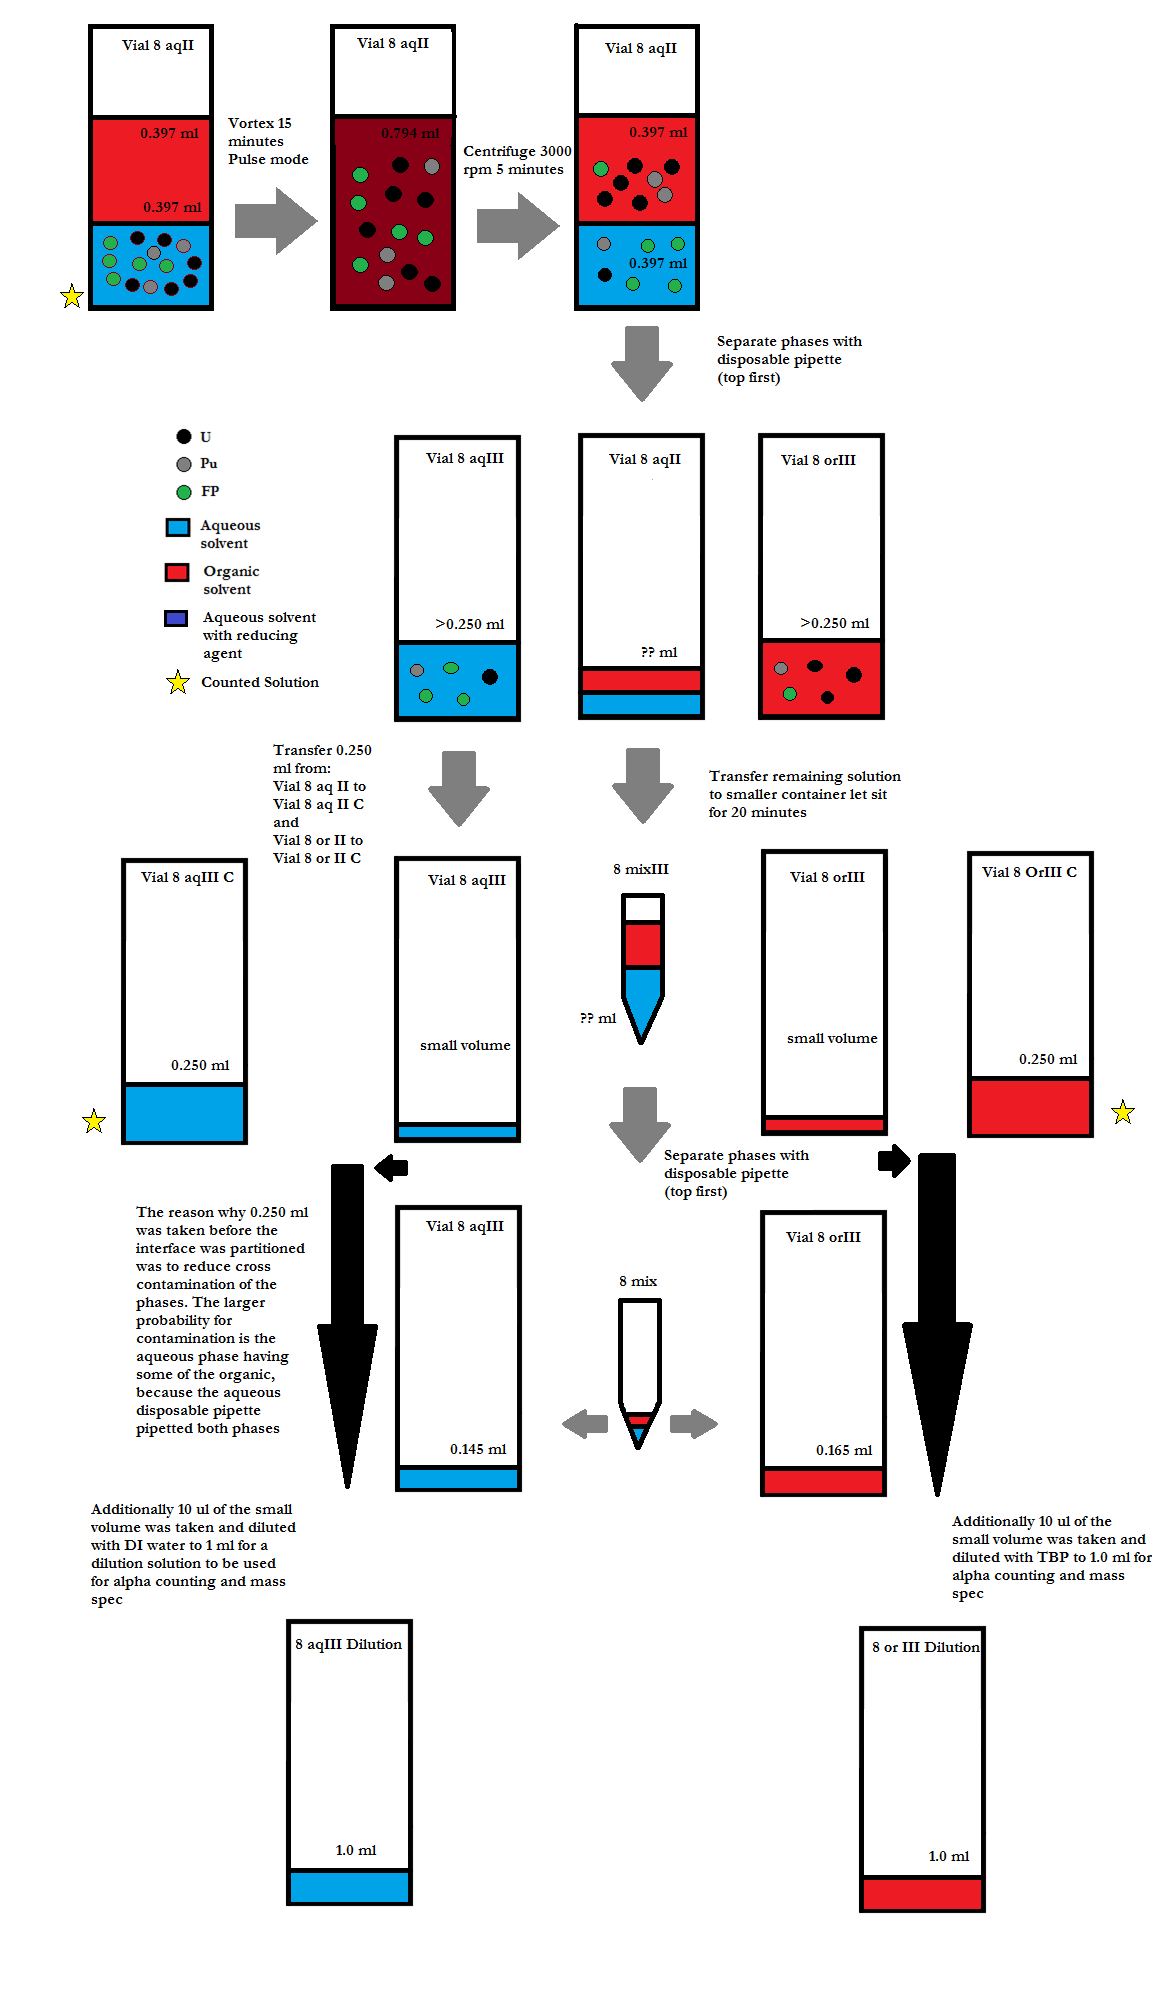
\includegraphics[width=0.8\linewidth]
                  {Figures/Cycle_x3_round_2_extraction_3}
\end{center}
\caption{Back extraction I, (different vial names, same procedure)}
\label{fig:round2_extraction3}
\end{figure}



%-----------------------------------------------------------------
%	LAB BOOK day
%---------------------------------------------------------------

\labday{Wednesday 21 December 2016, to January 5th, 2017}

\experiment{Process_X3}

\textbf{Counting}

Counting of all the samples. There were lots of aqueous samples to count.

During this time I also visited family. I completed my incomplete
for NUEN629, which came about because of a shattered kneecap.

%-----------------------------------------------------------------
%	LAB BOOK day
%---------------------------------------------------------------

\labday{Wednesday January 18th, 2017}

\experiment{Process_X3}

Analyzed data for experiments. Went to lab meeting and left
kind of angry, went home to cool off.

%-----------------------------------------------------------------
%	LAB BOOK day
%---------------------------------------------------------------

\labday{Thursday January 19th, 2017}

\experiment{Alpha_and_MassSpec}

Make chips...First reanalyzed the alpha spec, and now
the initial results are giving me about what I expect for \tss{239}Pu,
\tss{240}Pu, and \tss{241}Am. Now will analyze the D values for the
first extraction. Also note that redoing the alpha calculation took
all morning from 8-12 today. This included looking up alpha energies that
would overlap in my alpha spectrum. Analyzing the feasibility of having
\tss{238}Pu as a contributor in the alpha spectrum. Then doing an estimate
on what percent of the mass is \tss{238}Pu as opposed to \tss{241}Am.
Then checking whether the results for mass of \tss{238}Pu and \tss{241}Am
made sense (which required another estimate - as well as some calculations
from the mass spec).\\

\textbf{Some notes from the above}
\begin{equation*}
\text{Dilution Factor}=\frac{\text{Final Volume}}{\text{Initial Volume}}
\end{equation*}
Vials 8,9,10 dilute by another factor of 2 (really liked by detector).\\
Vials 8aq, 9aq, and 10aq Diluted by another factor of 4\\~\\

\begin{center}
\textbf{Mass Spec results comparison to 30G trace original}
\end{center}
Calculation expample for 5.63E-8 factor (assuming the density is 1.127 g, because
we don't know the volume they measured, just the mass)
\begin{equation*}
  \frac{ng}{g\ sample}\cdot0.0443\ \text{g sample}\cdot\frac{5.0\text{ ml (for 1/10)}}
       {0.039308\ \text{ml sent}}\cdot10\text{ (for other 10 parts)}\cdot
       \frac{10^{-9}\ g}{ng}=\frac{n}{\ sample}\cdot5.63E-8
\end{equation*}
Below is a table for masses in the stock for each mass bin.
Assuming mass ratios for a typical PWR at the same burnup (used below calculation)
\begin{equation*}
  \frac{6.02E23\text{ atoms}}{136\text{ g \tss{137}Cs}}\cdot
  \frac{\text{fission}}{0.06 \text{ atoms \tss{137}Cs}}
  \cdot\frac{200\ MeV}{\text{fission}}\cdot\frac{1.602E-19\ MJ}{MeV}\cdot\frac{1\ day}{86400\ s}
\end{equation*}
\begin{equation*}
  =27.1674\frac{MW\cdot day}{\text{g \tss{137}Cs}}
\end{equation*}
If we assume that burnup is 4000 MWd/t, then grams of \tss{137}Cs per ton HM should be 147.235.
\begin{table}[H]
\begin{center}
\begin{tabular}{l l l l}
\toprule
\textbf{Mass Bin} & \textbf{ng/g}& \textbf{x 5.63E-8 (g)} & \textbf{Constituents w Mass Frac}\\
\toprule
238 & 277000 & 0.0156 & \tss{238}U$\sim$1 \tss{238}Pu 6.44E-7\\
239 & 4330 & 2.44E-4 & \tss{239}Pu$\sim$1\\
240 & 362  & 2.04E-5 & \tss{240}Pu$\sim$1\\
241 & 150  & 8.45E-6 & \tss{241}Pu 0.9965 \tss{241}Am 3.53E-3\\
242 & 8.71 & 4.91E-7 & \tss{242}Pu 0.9952 \tss{242}Cm 4.75E-3\\
243 & 0.15 & 8.34E-9 & \tss{243}Am 0.9993 \tss{243}Cm 6.83E-4\\
& & & \tss{238}Pu 0.8565\tss{241}Am 0.14346\\
& & & \tss{239}Pu 92.29 \tss{240}Pu 0.07711\\
\bottomrule
\end{tabular}
\caption{The effects of treatments X and Y on the four groups studied.}
\label{tab:treatments_xy}
\end{center}
\end{table}

Below is summary for the alpha peaks 
\begin{table}[H]
\begin{center}
\begin{tabular}{l l l l}
\toprule
\textbf{Peak} & \textbf{Isotopes}& \textbf{Half-Life (years)} \\
\toprule
1st & \tss{239}Pu \tss{240}Pu & 24,110; 6,561\\
2nd & \tss{238}Pu \tss{241}Am & 87.7; 432.6\\
3rd & \tss{243}Cm & 29.1\\
4th & \tss{242}Cm & 0.446\\
\bottomrule
\end{tabular}
\caption{The effects of treatments X and Y on the four groups studied.}
\label{tab:treatments_xy}
\end{center}
\end{table}



\textbf{Prepare for dilution}
\begin{todolist}
\item[\done]{Label vials,
  $\boxed{8,9,10\ DilutionII}$,
  $\boxed{8\ aq\ DilutionII}$,
  $\boxed{9\ aq\ DilutionII}$,
  $\boxed{10\ aq\ DilutionII}$,
  (smaller twist cap (about 2ml) vials from John Burns)
  $\boxed{8\ ChipII}$, $\boxed{9\ ChipII}$,
  $\boxed{10\ ChipII}$,
  $\boxed{8aq\ ChipII}$,
  $\boxed{9aq\ ChipII}$,
  $\boxed{10aq\ ChipII}$,
  (little chips to dissolve solutions onto)}
\item[\done]{Transfer:
  $\boxed{8,9,10\ DilutionII}$,
  $\boxed{8\ aq\ DilutionII}$,
  $\boxed{9\ aq\ DilutionII}$,
  $\boxed{10\ aq\ DilutionII}$,
  with
  (their own spin cap)
  $\boxed{8\ ChipII}$, $\boxed{8\ ChipII}$,
  $\boxed{8\ ChipII}$,
  $\boxed{8aq\ ChipII}$,
  $\boxed{9aq\ ChipII}$,
  $\boxed{10aq\ ChipII}$, into glovebox in large plastic bag}
\end{todolist}

\textbf{Perform Dilution and make chips}

\begin{todolist}
\item[\done]{Main solution Dilution}
\begin{center}
  0.5+/-0.0075 ml of $\boxed{8,9,10\ Dilution}$ (0 M HNO\tsbs{3})
  [smaller pipette]\\
+\\
0.5+/-0.0075 ml of DI water (leftover in glovebox)\\
=\\
1+/-0.01 ml of $\sim$ 0 M HNO\tsbs{3} $\boxed{8,9,10\ DilutionII}$
\end{center}
\vspace{0.3cm}
\begin{center}
  20+/-0.2 $\mu$l of $\boxed{8,9,10\ DilutionII}$ dropped onto
  $\boxed{8\ ChipII}$
\end{center}
\begin{center}
  20+/-0.2 $\mu$l of $\boxed{8,9,10\ DilutionII}$ dropped onto
  $\boxed{9\ ChipII}$
\end{center}
\begin{center}
  20+/-0.2 $\mu$l of $\boxed{8,9,10\ DilutionII}$ dropped onto
  $\boxed{10\ ChipII}$
\end{center}

\item[\done]{Make second dilution of each aqueous (ExI)}
  \begin{todolist}
  \item[\done]{- $\boxed{8\ aq}$}
  \end{todolist}
  \begin{center}
    125+/-3.75 $\mu$l of $\boxed{8\ aq\ Dilution}$
    (0 M HNO\tsbs{3})\\
    +\\
    375+/-7.5 $\mu$l of DI water (leftover in glovebox)\\
    =\\
    0.5+/-0.0084 ml of $\sim$
    0 M HNO\tsbs{3} $\boxed{8\ aq\ DilutionII}$
  \end{center}
  \begin{center}
  20+/-0.2 $\mu$l of $\boxed{8\ aq\ DilutionII}$ dropped onto
  $\boxed{8\ Aq\ ChipII}$
  \end{center}
  \begin{todolist}
  \item[\done]{- $\boxed{9\ aq}$}
  \end{todolist}
  \begin{center}
    125+/-3.75 $\mu$l of $\boxed{9\ aq\ Dilution}$
    (0 M HNO\tsbs{3})\\
    +\\
    375+/-7.5 $\mu$l of DI water (leftover in glovebox)\\
    =\\
    0.5+/-0.0084 ml of $\sim$
    0 M HNO\tsbs{3} $\boxed{9\ aqBIII\ Dilution}$
  \end{center}
  \begin{center}
  20+/-0.2 $\mu$l of $\boxed{9\ aq\ DilutionII}$ dropped onto
  $\boxed{9\ Aq\ ChipII}$
  \end{center}
  \begin{todolist}
  \item[\done]{- $\boxed{10\ aq}$}
  \end{todolist}
  \begin{center}
    125+/-3.75 $\mu$l of $\boxed{10\ aq\ Dilution}$
    (0 M HNO\tsbs{3})\\
    +\\
    375+/-7.5 $\mu$l of DI water (leftover in glovebox)\\
    =\\
    0.5+/-0.0084 ml of $\sim$
    0 M HNO\tsbs{3} $\boxed{10\ aqBIII\ Dilution}$
  \end{center}
  \begin{center}
  20+/-0.2 $\mu$l of $\boxed{10\ aq\ DilutionII}$ dropped onto
  $\boxed{10\ Aq\ ChipII}$
  \end{center}
\end{todolist}

\textbf{Let Chips Dry}

\textbf{Combine final aqueous}
\begin{todolist}
\item[\done]{Transfer in glovebox $\boxed{8\ aqBIIIC}$,
  $\boxed{9\ aqBIIIC}$,
  $\boxed{10\ aqBIIIC}$,
  $\boxed{8\ aqBIIC}$,
  $\boxed{9\ aqBIIC}$,
  $\boxed{10\ aqBIIC}$,
  $\boxed{8\ aqBC}$,
  $\boxed{9\ aqBC}$,
  $\boxed{10\ aqBC}$}
\item[\done]{Combine all 8, 9 10 solutions into their respective stream
  in $\boxed{8\ aqBC}$, $\boxed{9\ aqBC}$, and $\boxed{10\ aqBC}$}
\item[\done]{Transfer out $\boxed{8\ aqBC}$, $\boxed{9\ aqBC}$, and $\boxed{10\ aqBC}$}
\item[\done]{Recount $\boxed{8\ aq\ BIII}$ (short count time - then combined)}
\end{todolist}

\experiment{CHEMLAB}

Attend Lab trainning. Took a lot longer than expected, but now trained to train the
youngins




%-----------------------------------------------------------------
%	LAB BOOK day
%---------------------------------------------------------------

\labday{Friday January 20th, 2017}

\experiment{Alpha_and_MassSpec}

\begin{todolist}
\item[\done]{Start alpha count $\boxed{9\ aq\ ChipII}$}
\item[\done]{Start count for $\boxed{8\ aqB\ tot}$}
\item[\done]{Stop alpha count $\boxed{9\ aq\ ChipII}$}
\item[\done]{Start alpha count $\boxed{8\ ChipII}$}  
\end{todolist}

\textbf{Transfer all samples to twist cap.} \\

This was a very long process of
relabeling all the dilution solutions, and putting them in smaller vials
with twist tops. They are now all stored in the fumehood by extraction
step (a big 50 ml tube for each step)\\

\textbf{Credit card fraud and lost student ID, left early to take care of}


%-----------------------------------------------------------------
%	LAB BOOK day
%---------------------------------------------------------------

\labday{Saturday January 21, 2017}

\experiment{Alpha_and_MassSpec}

\textbf{Counting}
\begin{todolist}
\item[\done]{Stop alpha count $\boxed{8\ ChipII}$}
\item[\done]{Start alpha count $\boxed{9\ ChipII}$}
\item[\done]{Stop alpha count $\boxed{9\ ChipII}$}
\item[\done]{Start alpha count $\boxed{10\ ChipII}$}
\item[\done]{Stop alpha count $\boxed{10\ ChipII}$}
\item[\done]{Start alpha count $\boxed{8\ Aq\ ChipII}$}
  
\item[\done]{Stop gamma count for $\boxed{8\ aqB\ tot}$}
\item[\done]{Start gamma count $\boxed{9\ aqB\ tot}$}
\end{todolist}

\textbf{Analyze Results}

\begin{todolist}
\item[\done]{Modified alpha spec program to calculate Cm.}
  \begin{itemize}
  \item{Bad results, but wasn't expecting much}
  \end{itemize}
\item[\done]{Analyzed magic concentration for Pu.}
  \begin{itemize}
  \item{Dilute Paul's solution by a factor of 200}
  \end{itemize}
\end{todolist}

\experiment{CHEMLAB}

Set up stuff for CHEM lab next week. (prelab, presentations, grading, blah)

%-----------------------------------------------------------------
%	LAB BOOK day
%---------------------------------------------------------------

\labday{Sunday January 22, 2017}

\experiment{Alpha_and_MassSpec}

\textbf{Counting Alpha}
\begin{todolist}
\item[\done]{Stop alpha count $\boxed{8\ Aq\ ChipII}$}
\item[\done]{Start alpha count $\boxed{10\ Aq\ ChipII}$}
  \begin{itemize}
  \item{The results from the alpha counts still have large tails, no good!}
  \end{itemize}
\end{todolist}

\textbf{Create alpha sample of $\boxed{8\ Aq}$ that is diluted again, maybe it will
        have good tails (third dilution of 8)}
\begin{todolist}
\item[\done]{- $\boxed{8\ aq}$}
\end{todolist}
\begin{center}
  300+/-6 $\mu$l of $\boxed{8\ aq\ DilutionII}$
  (0 M HNO\tsbs{3})\\
  +\\
  300+/-6 $\mu$l of DI water (leftover in glovebox)\\
  =\\
  0.6+/-0.0084 ml of $\sim$
  0 M HNO\tsbs{3} $\boxed{8\ aq\ DilutionII}$
\end{center}
\begin{center}
  20+/-0.2 $\mu$l of $\boxed{8\ aq\ Dilution3}$ dropped onto
  $\boxed{8\ Aq\ Chip3}$
\end{center}
\begin{todolist}
\item[\done]{Let $\boxed{8\ aq\ Chip3}$ Dry}
\item[\done]{Stop count of $\boxed{10\ Aq\ ChipII}$ (looked terrible anyway)}
\item[\done]{Start count of $\boxed{8\ Aq\ Chip3}$}
  \begin{itemize}
  \item{This count doesn't look too good either, I'm breaking sabbath  so I am leaving,
    Tomorrow after office hours I will dilute the sample once more}
  \end{itemize}
\end{todolist}

%-----------------------------------------------------------------
%	LAB BOOK day
%---------------------------------------------------------------

\labday{Monday January 23, 2017}

\experiment{Alpha_and_MassSpec}

\textbf{Create 4th dilution sample - Did all this in the glove box}
\begin{todolist}
\item[\done]{- $\boxed{8\ aq}$}
\end{todolist}
\begin{center}
  100+/-3 $\mu$l of $\boxed{8\ aq\ Dilution3}$
  (0 M HNO\tsbs{3})\\
  +\\
  300+/-3 $\mu$l of DI water (leftover in glovebox)\\
  =\\
  0.5+/-0.004 ml of $\sim$
  0 M HNO\tsbs{3} $\boxed{8\ aq\ Dilution4}$
\end{center}
\begin{center}
  20+/-0.2 $\mu$l of $\boxed{8\ aq\ Dilution4}$ dropped onto
  $\boxed{8\ Aq\ Chip4}$
\end{center}
\begin{todolist}
\item[\done]{Let $\boxed{8\ aq\ Chip4}$ Dry}
\item[\done]{Stop count of $\boxed{8\ Aq\ Chip3}$ (looked terrible anyway)}
\item[\done]{Start count of $\boxed{8\ Aq\ Chip4}$}
  \begin{itemize}
  \item{Dear Lord, Please let this work}
  \end{itemize}
\end{todolist}

\textbf{Hypotheses for why I am getting more counts than I expect from first extraction alpha}

I think I am getting more counts because even when I subtract as many counts as possible
and attribute them to \tss{241}Am, I still have too much plutonium.
\begin{itemize}
\item{Something wrong with experiment}
\item{HM on bottom of TBP}
\item{Uranium Backround in alpha}
\item{Spalation (causing multiple hits)}
\item{Calculating dilution factor incorrectly (I don't think I am)}
\item{Maybe sodium nitrite isn't working well, and I really only extracted
  a small portion of the plutonium}
\end{itemize}

\textbf{Calculation for converting gamma spec to closet solution}
\begin{equation*}
\frac{2.5ml}{0.4ml}\cdot10=62.5\ \text{Factor used}
\end{equation*}

\textbf{Used above calculation along with similiar for alpha and mass to make a list
  of elements and their closet solution masses at certain dates}\\~\\

\textbf{Proposal work - while sample drys and while at office hours}
\begin{todolist}
\item{List out all the things you want to put into your dissertation}
\item{Come up with a unifying theme}
\item{Write up the proposal}
\end{todolist}





%-----------------------------------------------------------------
%	LAB BOOK day
%---------------------------------------------------------------

\labday{Tuesday January 24, 2017}

\experiment{Alpha_and_MassSpec}


\textbf{Lets look at all the samples one after another}


\begin{figure}[H] % Example of including images
\begin{center}
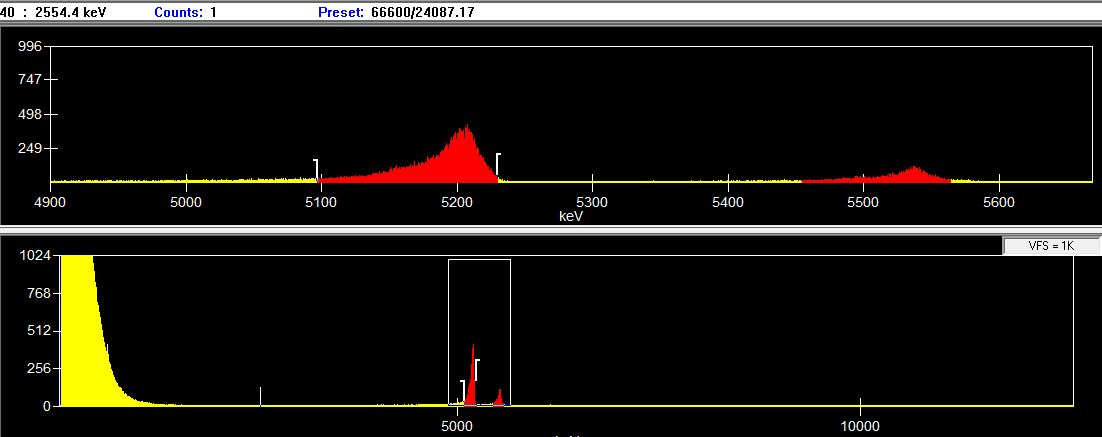
\includegraphics[width=0.9\linewidth]{Figures/Dilution1_Sample8}
\end{center}
\caption{Dilution factor of 40 Sample 8 first extraction}
\label{fig:example_figure}
\end{figure}

\begin{figure}[H] % Example of including images
\begin{center}
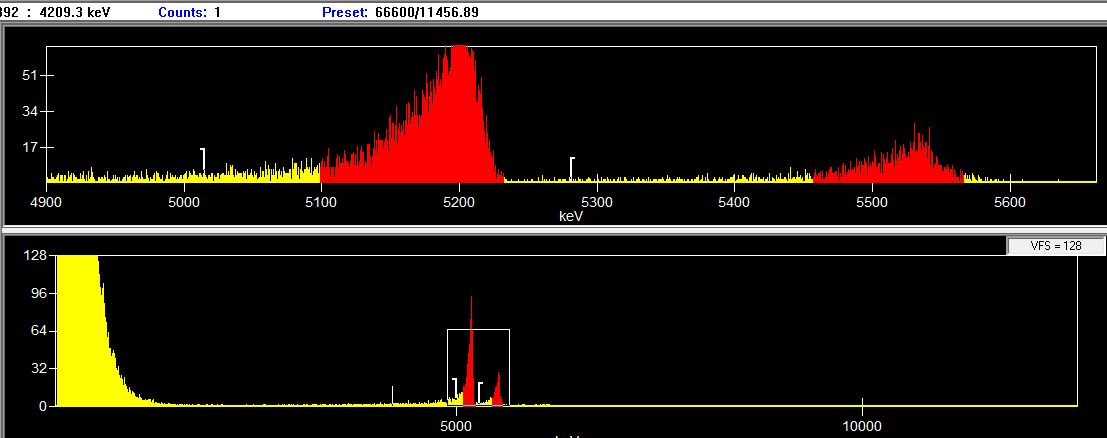
\includegraphics[width=0.9\linewidth]{Figures/Dilution2_Sample8}
\end{center}
\caption{Dilution factor of 160 Sample 8 first extraction}
\label{fig:example_figure}
\end{figure}

\begin{figure}[H] % Example of including images
\begin{center}
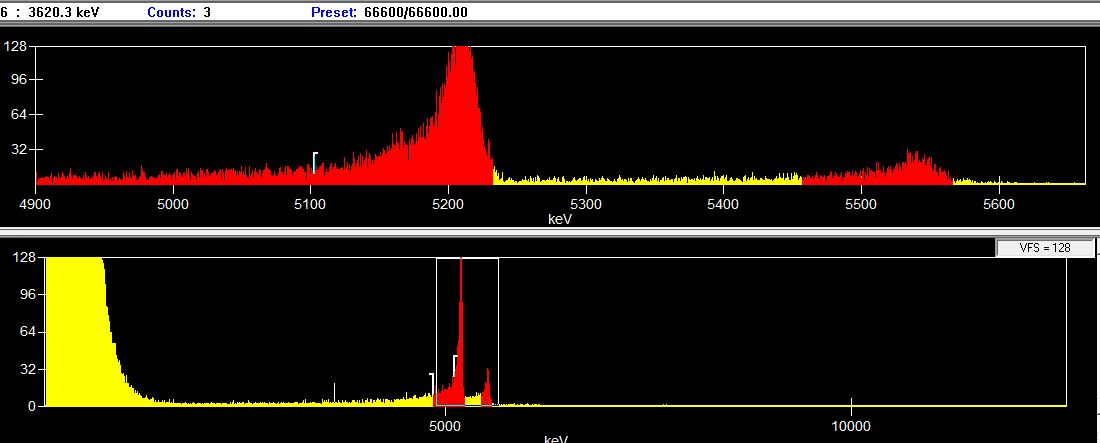
\includegraphics[width=0.9\linewidth]{Figures/Dilution3_Sample8}
\end{center}
\caption{Dilution factor of 320 Sample 8 first extraction}
\label{fig:example_figure}
\end{figure}


\begin{figure}[H] % Example of including images
\begin{center}
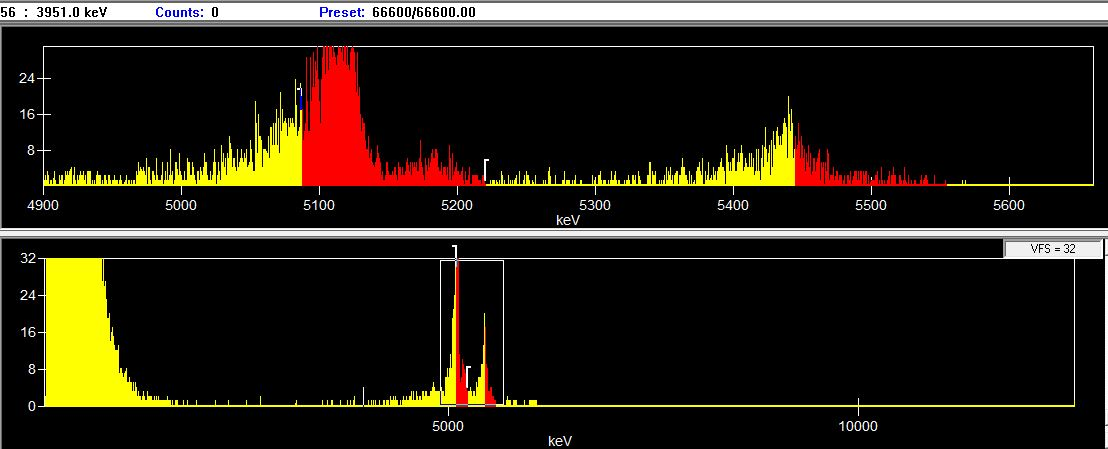
\includegraphics[width=0.9\linewidth]{Figures/Dilution4_Sample8}
\end{center}
\caption{Dilution factor of 1600 Sample 8 first extraction}
\label{fig:example_figure}
\end{figure}

\textbf{What the heck is the third peak?! Why energy shift?!}

This is troubling, very troubling. I spent the most of the rest of
the day trying to figure this out. I am not sure what it is.

\experiment{CHEMLAB}

Taught two classes today of CHEM Lab, which is technically 6 hours
of my day, should count for something.

%-----------------------------------------------------------------
%	LAB BOOK day
%---------------------------------------------------------------

\labday{Wednesday January 25, 2017}

\experiment{Alpha_and_MassSpec}

Spent most of the morning trying again to figure out what
is going on in the peaks, to no avail. Last night I was
feeling restless, so I wrote a program to parse and organize
data from the yellow site to help with this problem,
the program helped me organize alpha information, but I still
don't know what is going on.

\experiment{ResearchMeeting}

Worked on powerpoint to get information for the research meeting,
maybe others will know what is going on...\\~\\

They didn't, but we have some good things to work on moving forward

\begin{itemize}
\item{Alpha counts for back extraction}
\item{Redo calculation form mass spec}
\item{Redo calculation with assumptions on Am241}
\item{Look up alpha information}
\item{Check with UV vis to see which oxidation state Pu is in}
\item{Contact MURR for mass spec}
\end{itemize}

\textbf{Work after meeting}


\experiment{Alpha_and_MassSpec}

\begin{todolist}
\item[\done]{Make sample of $\boxed{8\ BExI\ Dilution}$ by dropping
  10 $\mu$l of $\boxed{8\ BExI\ Dilution}$ onto $\boxed{8\ BExI\ Chip}$}
\item[\done]{Let above chip dry}
\item[\done]{Start count of $\boxed{8\ BExI\ Chip}$}
\item[\done]{Look into Mass spec calculations, because there were accusations
  against how I calculated it, don't forget what the Dilution factor is}
\end{todolist}


%-----------------------------------------------------------------
%	LAB BOOK day
%---------------------------------------------------------------

\labday{Thursday January 26, 2017}

\experiment{Alpha_and_MassSpec}

\begin{todolist}
\item[\done]{Look into alpha spectrum from $\boxed{8\ BExI\ Chip}$, 4 peaks now
  (WTF!!)}
\item[\done]{Redid calculations for \tss{241}Am, and now need to redo alpha}
\end{todolist}


\experiment{CHEMLAB}

Taught one classes today of CHEM Lab and did lab practice for next week
, which is technically 6 hours
of my day, should count for something.



%-----------------------------------------------------------------
%	LAB BOOK day
%---------------------------------------------------------------

\labday{Friday January 27, 2017}

\experiment{Alpha_and_MassSpec}

\begin{todolist}
\item[\done]{Switchhed out alpha count $\boxed{8\ BExI\ Chip}$, to do a background}
\item[\done]{Started a background count for alpha to see if we have that as a problem}
  \begin{itemize}
  \item{Not a problem}
  \end{itemize}
\item[\done]{Recount a second dilution series (of the glovebox solution), to
  see if we have energy drift in the calibration}
\item[\done]{Explain the problem to Jason (who is smarter than me) and ask
  what he thinks, below are some things he brought up}
  \begin{itemize}
  \item{The ``bad'' spectrum is more of what we would expect, and the other
    ``good'' spectrum looks bad}
  \item{Maybe the more concentrated solutions shifted to the right because
    of coincidence with gamma rays (both FP and from alpha decay) - note that
    alpha decays usually instantly produce gamma rays}
  \item{Maybe there was drift in the detector while it was running}
  \item{The first set of samples had the detector running for a while, while the second didn't
    or vice versa}
  \end{itemize}
\item[\done]{Started recount of the solution that was diluted a factor of 320,
  to compare to the solution that was diluted to a factor for 1600, so they
  would have approximately the same number of counts}
\item[\done]{Summarized differences between mine and Matt's calculations,
  to show that I am not crazy in my mass spec, and to show that Matt's is probably wrong,
  at least with his density assumption}
\end{todolist}

\textbf{How many tons of material do we have?}
\begin{equation*}
0.0129g\cdot\frac{1ton}{10^6\ g}\cdot\frac{0.5\ ml}{5.167\ ml}\cdot\frac{0.4\ ml}{2.5\ ml}
\end{equation*}

%-----------------------------------------------------------------
%	LAB BOOK day
%---------------------------------------------------------------

\labday{Sunday January 29, 2017}

\experiment{Alpha_and_MassSpec}

\textbf{Expected Counts from Am241}
\begin{equation*}
  \frac{\text{Mass in Vial}}{\text{Dilution Factor}\cdot\text{Volume in Vial}}\cdot
  \frac{\text{Na}}{\text{M}}\cdot\lambda\cdot\epsilon
\end{equation*}




%-----------------------------------------------------------------
%	LAB BOOK day
%---------------------------------------------------------------

\labday{Monday January 30, 2017}

\experiment{Alpha_and_MassSpec}

\textbf{Notes On working through calculation}
\begin{itemize}
\item{Finish the redo of the alpha calculations, \tss{239}Pu and \tss{240}Pu
  didn't change much, I also solidified my mass spec calculations, which
  I think are right}
\item{My alpha and gamma results weren't giving major agreement for \tss{241}Am,
  Kevin said he was getting better agreement when he got rid of the 39-40 keV
  calibration point...I did that, and it helps a bunch. The 45 keV calibration
  point has a count rate of something like 0.69, if you double this, then your alpha
  and gamma results would be in agreement, but this is dishonest}
\item{This means that 17-34\% of the 241 mass bin is \tss{241}Am}
\item{Also today reworked the alpha calibration, thinking it might be the issue,
  but I found that Kevin did it relatively correctly, I made a spread sheet,
  I also used the following equation (below), amount of a second isotope when it has
  another isotope feeding it, and when the isotope itself decays, and when you start with
some of the isotope to begin with}
\item{I am looking at the ``drift'' on the energy bins in the calibration dudes...
  and I am wondering what it is due to}
\item{Also calculating how much plutonium I get in the final solutions}
\end{itemize}
\begin{equation*}
  N_2=\frac{\lambda_1N_{1o}}{\lambda_2-\lambda_1}\left[e^{-\lambda_1t}-e^{-\lambda_2t}\right]
  +N_{2o}e^{-\lambda_2t}
\end{equation*}
\begin{itemize}
\item{Also used the two below equations for the calibration calculations}
\end{itemize}
\begin{equation*}
\frac{\text{Total Bq}}{\text{Tot Atoms}}=\sum At\%_i\lambda_i\ \ \text{For Pu}
\end{equation*}
\begin{equation*}
\text{\% Activity}_i=\frac{N_i\lambda_i}{\text{Tot Activity}}\ \ \text{For Cm}
\end{equation*}



\experiment{CHEMLAB}

Also Prep for this weeks and next weeks lab...I'm kind of nervous about it


%-----------------------------------------------------------------
%	LAB BOOK day
%---------------------------------------------------------------

\labday{Tuesday January 31, 2017}

\experiment{Alpha_and_MassSpec}

\textbf{Notes On working through calculation}
\begin{itemize}
\item{Figured out what was going on, the detector had drifted in energy
  calibration while counting, which brought up the four peaks, we got the
  4-peak calibration source and recalibrated}
\item{Also looked at efficiency, and it changed some, but not a lot}
\end{itemize}

\experiment{CHEMLAB}

Taught 6 hours of lab today


%-----------------------------------------------------------------
%	LAB BOOK day
%---------------------------------------------------------------

\labday{Wednesday Feb 1, 2017}

\experiment{Alpha_and_MassSpec}
\begin{todolist}
\item[\done]{Measure final volume of final aqueous solutions}
  \begin{itemize}
  \item{Estimated final volumes to be 1950 $\mu$l $\pm$100 $\mu$l}
  \item{Does this make sense? See table below for total volumes of each phase,
  yes these numbers kind of make sense.}
  \end{itemize}
\end{todolist}

\begin{table}[H]
\caption{Volume, in $\mu$l, of solution added to organic for each back extraction}
\begin{tabular}{l l l l}
\toprule
\textbf{Back Extraction I} & \textbf{Back Extraction II} & \textbf{Back Extraction III}
& \textbf{Total}\\
\toprule
888 & 760 & 618 & 2266\\
912 & 765 & 620 & 2297\\
863 & 765 & 620 & 2254\\
\bottomrule
\end{tabular}
\label{tab:treatments_xy}
\end{table}

\begin{todolist}
\item[\done]{Make Alpha chip of $\boxed{8\ BExaqII\ Dilution}$}
\begin{center}
  10+/-0.1 $\mu$l of $\boxed{8\ BExAqII\ Dilution}$ dropped onto
  $\boxed{8\ BExAqII\ Chip}$
\end{center}
\item[\done]{Make Alpha chip of $\boxed{8\ BExaqIII\ Dilution}$}
\begin{center}
  10+/-0.1 $\mu$l of $\boxed{8\ BExAqIII\ Dilution}$ dropped onto
  $\boxed{8\ BExAqIII\ Chip}$
\end{center}
\item[\done]{Start count of $\boxed{8\ BExII\ Chip}$}
  \begin{itemize}
  \item{Count rates are pretty low}
  \end{itemize}
\item[\done]{Make dilutions of total aqueous solutions}
  \begin{todolist}
  \item[\done]{- $\boxed{8\ aq\ tot}$}
  \end{todolist}
  \begin{center}
    10+/-0.1 $\mu$l of $\boxed{8\ aq\ tot}$
    (4 M HNO\tsbs{3})\\
    +\\
    990+/-9.9 $\mu$l of DI water (leftover in glovebox)\\
  =\\
  1+/-0.01 ml of $\sim$
  0 M HNO\tsbs{3} $\boxed{8\ aq\ tot\ Dilution}$
\end{center}
\begin{center}
  10+/-0.1 $\mu$l of $\boxed{8\ aq\ tot\ Dilution}$ dropped onto
  $\boxed{8\ Aq\ tot\ Chip}$
\end{center}
\begin{itemize}
\item{Not completely centered}
\end{itemize}

  \begin{todolist}
  \item[\done]{- $\boxed{9\ aq\ tot}$}
  \end{todolist}
  \begin{center}
    10+/-0.1 $\mu$l of $\boxed{9\ aq\ tot}$
    (4 M HNO\tsbs{3})\\
    +\\
    990+/-9.9 $\mu$l of DI water (leftover in glovebox)\\
  =\\
  1+/-0.01 ml of $\sim$
  0 M HNO\tsbs{3} $\boxed{9\ aq\ tot\ Dilution}$
\end{center}
\begin{center}
  10+/-0.1 $\mu$l of $\boxed{9\ aq\ tot\ Dilution}$ dropped onto
  $\boxed{9\ Aq\ tot\ Chip}$
\end{center}
\begin{itemize}
\item{Not completely centered}
\end{itemize}
  \begin{todolist}
  \item[\done]{- $\boxed{10\ aq\ tot}$}
  \end{todolist}
  \begin{center}
    10+/-0.1 $\mu$l of $\boxed{10\ aq\ tot}$
    (4 M HNO\tsbs{3})\\
    +\\
    990+/-9.9 $\mu$l of DI water (leftover in glovebox)\\
  =\\
  1+/-0.01 ml of $\sim$
  0 M HNO\tsbs{3} $\boxed{10\ aq\ tot\ Dilution}$
\end{center}
\begin{center}
  10+/-0.1 $\mu$l of $\boxed{10\ aq\ tot\ Dilution}$ dropped onto
  $\boxed{10\ Aq\ tot\ Chip}$
\end{center}
\begin{itemize}
\item{Not completely centered}
\end{itemize}
\end{todolist}


\begin{itemize}
\item{Redid calculations for alpha spectra, found that things
  aren't good, but at least are consistent}
\item{Went to research meeting, presented results, and surprisingly,
  they will let me continue, hopefully I will graduate soon}
\end{itemize}

\experiment{ResearchMeeting}{Details from research meeting}
\textbf{To Do for this week}
\begin{itemize}
\item{List of bulleted items}
\item{At least 2 journal paper references}
\item{Set up meeting with Gayle to ask about the project, these results are not so good}
\item{Send 50$\mu$l of sample, our results aren't the best}
\end{itemize}




%-----------------------------------------------------------------
%	LAB BOOK day
%---------------------------------------------------------------

\labday{Thursday February 2, 2017}


\experiment{CHEMLAB}

Taught 3 hours, did training for 3 hours, and worked on prelab


\experiment{Alpha_and_MassSpec}
\begin{todolist}
\item[\done]{Stop alpha $\boxed{8\ BExII\ Chip}$ count}
\item[\done]{Start alpha $\boxed{8\ BExIII\ Chip}$ count, really low count rate}
\end{todolist}

\experiment{Grad}

\begin{todolist}
\item[\done]{Calculate out when I will graduate and tell hiring person that is when
  I will start}
  \begin{itemize}
  \item{Probably the week of June 5th}
  \end{itemize}
\item[\done]{Email Alexis about this starting date}
\item{Write 3 pages of proposal}
\end{todolist}



%-----------------------------------------------------------------
%	LAB BOOK day
%---------------------------------------------------------------

\labday{Friday February 3, 2017}

\experiment{Grad}

\begin{todolist}
\item[\done]{Write proposal}
\end{todolist}
\textbf{Some things that came up while writing proposal}
\begin{itemize}
\item{What about different fast-to-thermal ratios, thermal-fast-epi,
  3 group, x-sections, compare to reactor types}
\item{Note that Jeremy's methodology works on all the waste solutions}
\item{Notes for paper and things already written but not included in paper}
  \begin{itemize}
  \item{Ru106, depletion Error}
  \item{attribution indicators, clue}
  \end{itemize}
\end{itemize}
\textbf{Depletion References Descriptions}
\begin{itemize}
\item{Reference 1}
  \begin{itemize}
  \item{BWR and PWR framework (zwermann)}
  \item{GRS sampling - I would probably use the same (XSUSA$\rightarrow$TRITON$\rightarrow$Scale)}
  \item{K$_\infty$, $\sigma$, with inventory $\sigma$}
  \item{Importance dudes}
  \end{itemize}
\item{Reference 2}
  \begin{itemize}
  \item{PWR Framework (Rochman) - Neverlands 2013}
  \item{Fast Total Monte Carlo, X-sections randomized}
  \item{SERPENT, K$_\infty$, RR, 2-group x-section}
  \item{Inventory, local pin power density, peturb and run through calculation}
  \item{TALLYS - nuclear reaction code - Random Nuclear data}
  \end{itemize}
\item{Reference 3}
  \begin{itemize}
  \item{Monte Carlo slow, two group, 2014}
  \item{Neutron spectrum variations}
  \item{Prepackaged, Fast Systems, Scale X-sections}
  \item{One Group or multigroup}
  \end{itemize}
\item{Reference 4}
  \begin{itemize}
  \item{Uncertainty Analysis Applied to fuel}
  \item{Depletion Calculations}
  \item{Statistical Approach}
  \item{CASMO-4 experimental data, MOX fuel}
  \end{itemize}
\item{Multiphysics nuclear reactor core depletion}
\item{I want to follow reference 2}
  \begin{itemize}
  \item{Unique x-sections, BC unique flux values}
  \end{itemize}
\end{itemize}


%-----------------------------------------------------------------
%	LAB BOOK day
%---------------------------------------------------------------


\labday{Sunday February 5, 2017}

\begin{todolist}
\item[\done]{Update notes for the week}
\end{todolist}


\experiment{CHEMLAB}

\begin{todolist}
\item[\done]{Start lab for next week}
\end{todolist}


%-----------------------------------------------------------------
%	LAB BOOK day
%---------------------------------------------------------------


\labday{Monday February 6, 2017}

\experiment{CHEMLAB}

\begin{todolist}
\item[\done]{Finish notes for lab}
\item[\done]{Office hours in the morning}
\end{todolist}

\experiment{Grad}

\begin{todolist}
\item[\done]{Assume constant flux or a monte carlo flux}
\item[\done]{What solutions do I need mass spec on}
  \begin{itemize}
  \item{Initial Solutions (8,9,10) three samples}
  \item{Final solutions (8,9,10) three samples}
  \item{First Extraction Aq solutions (8,9,10) Three samples}
  \item{Total of 9 samples}
  \end{itemize}
\end{todolist}


%-----------------------------------------------------------------
%	LAB BOOK day
%---------------------------------------------------------------


\labday{Tuesday February 7, 2017}

\experiment{CHEMLAB}

\begin{todolist}
\item[\done]{Teach two sections of lab today}
\item[\done]{Also got a bunch of laboratory reportst to grade}
\end{todolist}

\experiment{Alpha_and_MassSpec}

\textbf{Making alpha samples of diluted samples}
\begin{todolist}
\item[\done]{Extraction II}

  \begin{todolist}
  \item[\done]{- $\boxed{8\ AqII\ Dilution}$}
  \end{todolist}
  \vspace{0.3cm}
  \begin{center}
    10+/-0.12 $\mu$l of $\boxed{8\ AqII\ Dilution}$ dropped onto
    $\boxed{8\ ExII\ Chip\ DF100}$
  \end{center}
  
  \begin{todolist}
  \item[\done]{- $\boxed{9\ AqII\ Dilution}$}
  \end{todolist}
  \vspace{0.3cm}
  \begin{center}
    10+/-0.12 $\mu$l of $\boxed{9\ AqII\ Dilution}$ dropped onto
    $\boxed{9\ ExII\ Chip\ DF100}$
  \end{center}

  \begin{todolist}
  \item[\done]{- $\boxed{10\ AqII\ Dilution}$}
  \end{todolist}
  \vspace{0.3cm}
  \begin{center}
    10+/-0.12 $\mu$l of $\boxed{10\ AqII\ Dilution}$ dropped onto
    $\boxed{10\ ExII\ Chip\ DF100}$
  \end{center}

\item[\done]{Extraction III}

  \begin{todolist}
  \item[\done]{- $\boxed{8\ AqIII\ Dilution}$}
  \end{todolist}
  \vspace{0.3cm}
  \begin{center}
    10+/-0.12 $\mu$l of $\boxed{8\ AqIII\ Dilution}$ dropped onto
    $\boxed{8\ ExIII\ Chip\ DF100}$
  \end{center}
  
  \begin{todolist}
  \item[\done]{- $\boxed{9\ AqIII\ Dilution}$}
  \end{todolist}
  \vspace{0.3cm}
  \begin{center}
    10+/-0.12 $\mu$l of $\boxed{9\ AqIII\ Dilution}$ dropped onto
    $\boxed{9\ ExIII\ Chip\ DF100}$
  \end{center}

  \begin{todolist}
  \item[\done]{- $\boxed{10\ AqIII\ Dilution}$}
  \end{todolist}
  \vspace{0.3cm}
  \begin{center}
    10+/-0.12 $\mu$l of $\boxed{10\ AqIII\ Dilution}$ dropped onto
    $\boxed{10\ ExIII\ Chip\ DF100}$
  \end{center}

\item[\done]{Extraction 4}

  \begin{todolist}
  \item[\done]{- $\boxed{8\ A4\ Dilution}$}
  \end{todolist}
  \vspace{0.3cm}
  \begin{center}
    10+/-0.12 $\mu$l of $\boxed{8\ Aq4\ Dilution}$ dropped onto
    $\boxed{8\ Ex4\ Chip\ DF100}$
  \end{center}
  
  \begin{todolist}
  \item[\done]{- $\boxed{9\ Aq4\ Dilution}$}
  \end{todolist}
  \vspace{0.3cm}
  \begin{center}
    10+/-0.12 $\mu$l of $\boxed{9\ Aq4\ Dilution}$ dropped onto
    $\boxed{9\ Ex4\ Chip\ DF100}$
  \end{center}

  \begin{todolist}
  \item[\done]{- $\boxed{10\ Aq4\ Dilution}$}
  \end{todolist}
  \vspace{0.3cm}
  \begin{center}
    10+/-0.12 $\mu$l of $\boxed{10\ Aq4\ Dilution}$ dropped onto
    $\boxed{10\ Ex4\ Chip\ DF100}$
  \end{center}

\item[\done]{Back Extraction I}

  \begin{todolist}
  \item[\done]{- $\boxed{8\ AqBI\ Dilution}$}
  \end{todolist}
  \vspace{0.3cm}
  \begin{center}
    10+/-0.12 $\mu$l of $\boxed{8\ AqBI\ Dilution}$ dropped onto
    $\boxed{8\ ExBI\ Chip\ DF100}$
  \end{center}
  
  \begin{todolist}
  \item[\done]{- $\boxed{9\ AqBI\ Dilution}$}
  \end{todolist}
  \vspace{0.3cm}
  \begin{center}
    10+/-0.12 $\mu$l of $\boxed{9\ AqBI\ Dilution}$ dropped onto
    $\boxed{9\ ExBI\ Chip\ DF100}$
  \end{center}

  \begin{todolist}
  \item[\done]{- $\boxed{10\ AqBI\ Dilution}$}
  \end{todolist}
  \vspace{0.3cm}
  \begin{center}
    10+/-0.12 $\mu$l of $\boxed{10\ AqBI\ Dilution}$ dropped onto
    $\boxed{10\ ExBI\ Chip\ DF100}$
  \end{center}

\item[\done]{Back Extraction II}

  \begin{todolist}
  \item[\done]{- $\boxed{8\ AqBII\ Dilution}$}
  \end{todolist}
  \vspace{0.3cm}
  \begin{center}
    10+/-0.12 $\mu$l of $\boxed{8\ AqBII\ Dilution}$ dropped onto
    $\boxed{8\ ExBII\ Chip\ DF100}$
  \end{center}
  
  \begin{todolist}
  \item[\done]{- $\boxed{9\ AqBII\ Dilution}$}
  \end{todolist}
  \vspace{0.3cm}
  \begin{center}
    10+/-0.12 $\mu$l of $\boxed{9\ AqBII\ Dilution}$ dropped onto
    $\boxed{9\ ExBII\ Chip\ DF100}$
  \end{center}

  \begin{todolist}
  \item[\done]{- $\boxed{10\ AqBII\ Dilution}$}
  \end{todolist}
  \vspace{0.3cm}
  \begin{center}
    10+/-0.12 $\mu$l of $\boxed{10\ AqBII\ Dilution}$ dropped onto
    $\boxed{10\ ExBII\ Chip\ DF100}$
  \end{center}

\item[\done]{Back Extraction III}

  \begin{todolist}
  \item[\done]{- $\boxed{8\ AqBIII\ Dilution}$}
  \end{todolist}
  \vspace{0.3cm}
  \begin{center}
    10+/-0.12 $\mu$l of $\boxed{8\ AqBIII\ Dilution}$ dropped onto
    $\boxed{8\ ExBIII\ Chip\ DF100}$
  \end{center}
  
  \begin{todolist}
  \item[\done]{- $\boxed{9\ AqBIII\ Dilution}$}
  \end{todolist}
  \vspace{0.3cm}
  \begin{center}
    10+/-0.12 $\mu$l of $\boxed{9\ AqBIII\ Dilution}$ dropped onto
    $\boxed{9\ ExBIII\ Chip\ DF100}$
  \end{center}

  \begin{todolist}
  \item[\done]{- $\boxed{10\ AqBIII\ Dilution}$}
  \end{todolist}
  \vspace{0.3cm}
  \begin{center}
    10+/-0.12 $\mu$l of $\boxed{10\ AqBIII\ Dilution}$ dropped onto
    $\boxed{10\ ExBIII\ Chip\ DF100}$
  \end{center}

\item[\done]{Tot Product}

  \begin{todolist}
  \item[\done]{- $\boxed{8\ Tot\ Dilution}$}
  \end{todolist}
  \vspace{0.3cm}
  \begin{center}
    10+/-0.12 $\mu$l of $\boxed{8\ Tot\ Dilution}$ dropped onto
    $\boxed{8\ Tot\ Chip\ DF100}$
  \end{center}
  
  \begin{todolist}
  \item[\done]{- $\boxed{9\ Tot\ Dilution}$}
  \end{todolist}
  \vspace{0.3cm}
  \begin{center}
    10+/-0.12 $\mu$l of $\boxed{9\ Tot\ Dilution}$ dropped onto
    $\boxed{9\ Tot\ Chip\ DF100}$
  \end{center}

  \begin{todolist}
  \item[\done]{- $\boxed{10\ Tot\ Dilution}$}
  \end{todolist}
  \vspace{0.3cm}
  \begin{center}
    10+/-0.12 $\mu$l of $\boxed{10\ Tot\ Dilution}$ dropped onto
    $\boxed{10\ Tot\ Chip\ DF100}$
  \end{center}

\end{todolist}


\textbf{Counting}
\begin{todolist}
\item[\done]{Start alpha count $\boxed{8\ ExI\ Aq ChipII}$ (Extraction I Aqueous phase DF=160)}
  \begin{itemize}
  \item{Realize that we already counted $\boxed{8\ ExI\ Aq ChipII}$ and $\boxed{10\ ExI\ Aq ChipII}$}
  \end{itemize}
\item[\done]{Stop alpha count $\boxed{8\ ExI\ Aq ChipII}$}
\item[\done]{Start alpha count $\boxed{8\ Tot\ Aq}$}
\end{todolist}



%-----------------------------------------------------------------
%	LAB BOOK day
%---------------------------------------------------------------


\labday{Wednesday February 8, 2017}

\experiment{Alpha_and_MassSpec}
\begin{todolist}
\item[\done]{Stop alpha count $\boxed{8\ Tot\ Aq}$}
  \begin{itemize}
  \item{Noticed Energies were way off, but still two peaks}
  \end{itemize}
\item[\done]{Loaded up alpha source}
  \begin{itemize}
  \item{The energy peaks shifted back to what it should be! What?!}
  \end{itemize}
\item[\done]{Restarted alpha count $\boxed{8\ Tot\ Aq}$, and its energies are now
  in the right places....annoying}
\end{todolist}

\experiment{ResearchMeeting}
\textbf{Things to talk about for this last week}
\begin{itemize}
\item{Made all alpha samples}
\item{Will need three weeks with the 4 peak alpha source}
\item{Sent proposal to Dr. Chirayath Friday evening}
  \begin{itemize}
  \item{DF leading to Pu initial concentration}
    \begin{itemize}
    \item{Mathmatical determination of DF}
    \item{Use for next step}
    \end{itemize}
  \item{Forensic analysis for attribution indicators}
    \begin{itemize}
    \item{Burnup (Cs-137)}
    \item{Flux Magnitude (Nd-148)}
    \item{Initial enrichment (Heavy Metal Composition)}
    \item{Fuel Age (Burn-up)$\rightarrow$ concentration, decay}
    \item{Fast-to-thermal ratios (iterative solution)}
    \end{itemize}
  \end{itemize}
\item{Samples for mass spec}
  \begin{itemize}
  \item{Initial solutions Aq (3)}
  \item{First extraction Aq solutions (3)}
  \item{Final solutions (3)}
  \end{itemize}
\item{Calculated DFs}
\item{Kevin found a nice paper}
\item{Dr. Chirayath returned proposal (to committee members by end of week)}
\end{itemize}
\textbf{Results from Research Meeting}

\begin{todolist}
\item{Mass balance with organic \frownie}
  \begin{itemize}
  \item{Add drop of concentrated nitric acid to diluted aqueous phases}
  \item{Let sit over the weekend, make samples of it}
  \end{itemize}
\item[\done]{Ask prophessors about a defense date for the proposal}
\item{Normalize results to volume}
\item{Figure out 40 keV peak}
\item{Average runs accross}
\item{Finish Paper for proposal}
\item{ph versus plutonium oxidation states}
\end{todolist}
\textbf{Interesting thing from Jeremy's stuff}
\begin{itemize}
\item{What is the covariance between two ratios}
\item{Xe declarations, Charlton paper, correlated between burnup and reactor type}
\end{itemize}

\experiment{Alpha_and_MassSpec}
\textbf{Counting}
\begin{todolist}
\item[\done]{Stop alpha count $\boxed{8\ Tot\ Aq}$}
\item[\done]{Start alpha count $\boxed{9\ Tot\ Aq}$}
  \begin{itemize}
  \item{The energy peaks look off, but I have two samples with one on, and one off
    hopefully they give the same answers}
  \end{itemize}
\end{todolist}
\textbf{Counting}
\begin{todolist}
\item[\done]{Find which samples you can add a small amount of concentrated nitric acid to}
  \begin{itemize}
  \item{Should add to organic total diluted samples, they have a DF of 100, and were
    diluted in DI water}
  \end{itemize}
\end{todolist}
\textbf{Prepping the organic solutions, final concentration of nitric acid should be 0.5 M}
\begin{align*}
  m_1V_1=&m_2V_2\\
  V_1=&\frac{m_2V_2}{m_1}\\
  V_1=&\frac{0.5*1.0334}{15.44}\\
  V_1=&0.0334
\end{align*}
This means we should add 33.4 $\mu$l of concentrated nitric acid to our organic total
diluted solutions.
\begin{todolist}
\item[\done]{Add 33.4 of 15.44 M HNO\tsbs{3} to $\boxed{8\ Or\ Tot\ Dilution}$}
\item[\done]{Add 33.4 of 15.44 M HNO\tsbs{3} to $\boxed{9\ Or\ Tot\ Dilution}$}
\item[\done]{Add 33.4 of 15.44 M HNO\tsbs{3} to $\boxed{10\ Or\ Tot\ Dilution}$}
\end{todolist}
%----------------------------------------------------------------------
%	Examples
%-----------------------------------------------------------------------

%\smiley
%\frownie

%---------------------------------------
% Blank template to use for new days:
%---------------------------------------
%\labday{Day, Date Month Year}
%\experiment{}
%Text

%---------------------------------------
% To do list
%---------------------------------------
%% \begin{todolist}
%% \item[\wontfix]{profit}
%% \item[\done]{This is done}
%% \item{This is not done}
%% \end{todolist}

%---------------------------------------
% Vial Step
%---------------------------------------
%% \begin{todolist}
%% \item{-}
%% \end{todolist}
%% \begin{center}
%% Vial 1\\
%% +\\
%% Vial 2\\
%% =\\
%% Final Vial
%% \end{center}

%% \labday{Example} % We don't want a date here so we make the labday blank

%% \begin{center}
%% \HRule \\[0.4cm]
%% {\huge \textbf{Examples}}\\[0.4cm] % Heading
%% \HRule \\[1.5cm]
%% \end{center}

%% %-----------------------------------------------------------------------
%% %	Formulae
%% %-----------------------------------------------------------------------
%% \huge \textbf{Formulae} \\ \\

%% \normalsize \textbf{Formula 1 - Pythagorean theorem}\\ \\
%% $a^2 + b^2 = c^2$\\ \\

%% %--------------------------------------------------------------
%% %	Citation
%% %--------------------------------------------------------------

%% Citation test \cite{Tatro2013}.

%% %--------------------------------------------------------------
%% %	Figure
%% %--------------------------------------------------------------

%% \begin{figure}[H] % Example of including images
%% \begin{center}
%% 
\includegraphics[width=0.5\linewidth]{Figures/example_figure}
%% \end{center}
%% \caption{Example figure.}
%% \label{fig:example_figure}
%% \end{figure}

%% %--------------------------------------------------------------
%% %	Table
%% %--------------------------------------------------------------

%% \experiment{table}

%% \begin{table}[H]
%% \begin{tabular}{l l l}
%% \toprule
%% \textbf{Groups} & \textbf{Treatment X} & \textbf{Treatment Y} \\
%% \toprule
%% 1 & 0.2 & 0.8\\
%% 2 & 0.17 & 0.7\\
%% 3 & 0.24 & 0.75\\
%% 4 & 0.68 & 0.3\\
%% \bottomrule
%% \end{tabular}
%% \caption{The effects of treatments X and Y on the four groups studied.}
%% \label{tab:treatments_xy}
%% \end{table}

%% Table \ref{tab:treatments_xy} shows that groups 1-3 reacted similarly to the two treatments but group 4 showed a reversed reaction.

%% %------------------------------------------------------------
%% %	Bibliography
%% %------------------------------------------------------------
%% \bibliography{references} 
%% \bibliographystyle{plain} 

\end{document}

